\documentclass[11pt]{article}
\usepackage[utf8]{inputenc}
\usepackage[spanish]{babel}
\usepackage{geometry}
\usepackage{graphicx}
\usepackage{float}
\usepackage{amsmath}
\usepackage{booktabs}
\usepackage{hyperref}
\usepackage{array}
\usepackage{tabularx}
\usepackage[affil-it]{authblk}
\usepackage{longtable}
\usepackage{array}
\usepackage{enumitem}

\geometry{margin=1in}
\graphicspath{{./}}

\title{Proyecto 1: Análisis AC de filtro activo con agente SPICE educativo}
\author{Alumno: Johan Garcia Torres.      {\small Maestro: Dr. Francisco Elias Rangel Patiño.}}
\affil{Instituto Tecnológico de Jalisco, Maestría en Ingeniería en Electrónica.}
\date{\today}

\begin{document}
\maketitle

\section*{Resumen ejecutivo}
El presente reporte documenta la comparación entre el análisis AC realizado con las herramientas del agente SPICE educativo y la referencia generada con HSPICE. El análisis se realizará en tres circuitos: 
\begin{enumerate}
	\item Circuito objetivo 
	\item Circuito objetivo con valores diferentes 
	\item Circuito diferente
\end{enumerate}

Para el análisis de los amplificadores operacionales el agente usa un model de analisis nodal modificado (MNA - Modified Nodal Analisys)Se hace un barrido en frecuencia por parte del agente y se compara con la referencia HSPICE.

\section{Objetivo y alcance}
El objetivo de esta práctica es evaluar los resultados de un agente SPICE creado en clase con respecto a los resultados del programa HSPICE para el analisis de circuitos no tan complejos. Teniendo en cuenta que los elementos representan comportamientos ideales del analisis de circuitos. El analisis de AC contempla un barrido en frecuencia.
Los entregables por parte del agente son los siguientes:

\begin{enumerate}
	\item Validación: análisis MNA(para el caso de los OpAmps), barrido LIN de 300 puntos entre 10 Hz y 100 kHz. Función de transferencia: $H(w)= \frac{VOUT}{VIN}$.
	\item Gráficas: magnitud en dB, magnitud de V(N\_OUT) en voltios y fase.
	\item Esquema y matrices: esquemático, grafo con la restricción ideal visible, matriz de Tableau incluyendo las matrices Y/Z/W .El Tableau es parcial cuando se incluye op-amp ideal, dado que el analisis se resuelve con MNA.
	\item Reporte: reporte\_ac.md incluye las tres gráficas y los valores por frecuencia para los 300 puntos.
\end{enumerate}

\section{Metodología aplicada}
La metodología sigue la arquitectura y las puertas de validación descritas en la \textit{Guía Metodológica} (flujo funcional de la sección 1.1 y \textit{guardrails} de las secciones 4 y 6). PLAN\_01 organiza la definición y dependencias de las herramientas; PLAN\_02 describe su integración, selección de formulación, validación y comparación con referencias. Estos planes orientan el flujo, mientras que los resultados reportados proceden de los artefactos de la ejecución del circuito.

\begin{enumerate}
  \item \textbf{Entrada y alcance.} Se tomó el netlist \texttt{circuito\_objetivo.cir}, con referencia \texttt{0}, excitación AC de 1 mV y observable acordado $V(N OUT)/V(N IN)$ en el barrido lineal de 300 puntos entre 10 Hz y 100 kHz.
  \item \textbf{Puerta de validación del netlist.} \texttt{validate\_netlist.py} terminó en \textbf{Satisfactoriamente} con cero diagnósticos. Conforme a la metodología, un FAIL habría detenido el flujo antes de construir el circuito.
  \item \textbf{Parseo y modelo.} \texttt{parse\_netlist.py} generó la representación estructurada con valores en unidades SI. \texttt{build\_circuit\_model.py} conservó la identidad de componentes, el orden determinista de nodos y ramas y el op-amp como dispositivo aparte.
  \item \textbf{Topología.} \texttt{build\_oriented\_graph.py} produjo el grafo dirigido. \texttt{build\_incidence\_matrix.py} generó la matriz de incidencia reducida. La orientación sigue el orden de terminales del netlist y $+1/-1$ indica rama saliente/entrante, respectivamente.
  \item \textbf{Selección de formulación.} Debido a \texttt{.OPAMP U1 NP NM OUT IDEAL}, se eligió exclusivamente MNA. En el modelo lineal ideal del proyecto las corrientes de entrada son cero, $V(NP)=V(NM)$ y se incorpora una corriente auxiliar de salida. No se modelan rieles ni saturación; el op-amp no se sustituye por una rama pasiva.
  \item \textbf{Ensamble y barrido.} \texttt{build\_mna\_system.py} produjo el sistema complejo MNA de $7\times7$ para 10 Hz. \texttt{solve\_ac\_sweep.py} ejecutó el barrido completo en MNA y produjo las transferencias, magnitudes, dB y fases por frecuencia.
  \item \textbf{Validación de solución.} Se revisaron estados de solver y validación en cada frecuencia. El resultado fue \textbf{Satisfactorio} globalmente en los 300 puntos; el residuo lineal reportado varió entre $1.59\times10^{-24}$ y $5.16\times10^{-20}$. La solución sólo se considera aceptada por este estado y por los controles internos reportados.
  \item \textbf{Comparación externa y presentación.} Se usó el listado HSPICE existente como referencia, sin interpolar frecuencias. \texttt{compare\_reference.py} comparó únicamente los dos puntos con frecuencia exactamente coincidente (10 Hz y 100 kHz); ambos pasaron con las tolerancias declaradas en el artefacto. Luego se incorporaron la topología y las gráficas de los resultados disponibles.
\end{enumerate}

\begin{figure}[H]
\centering
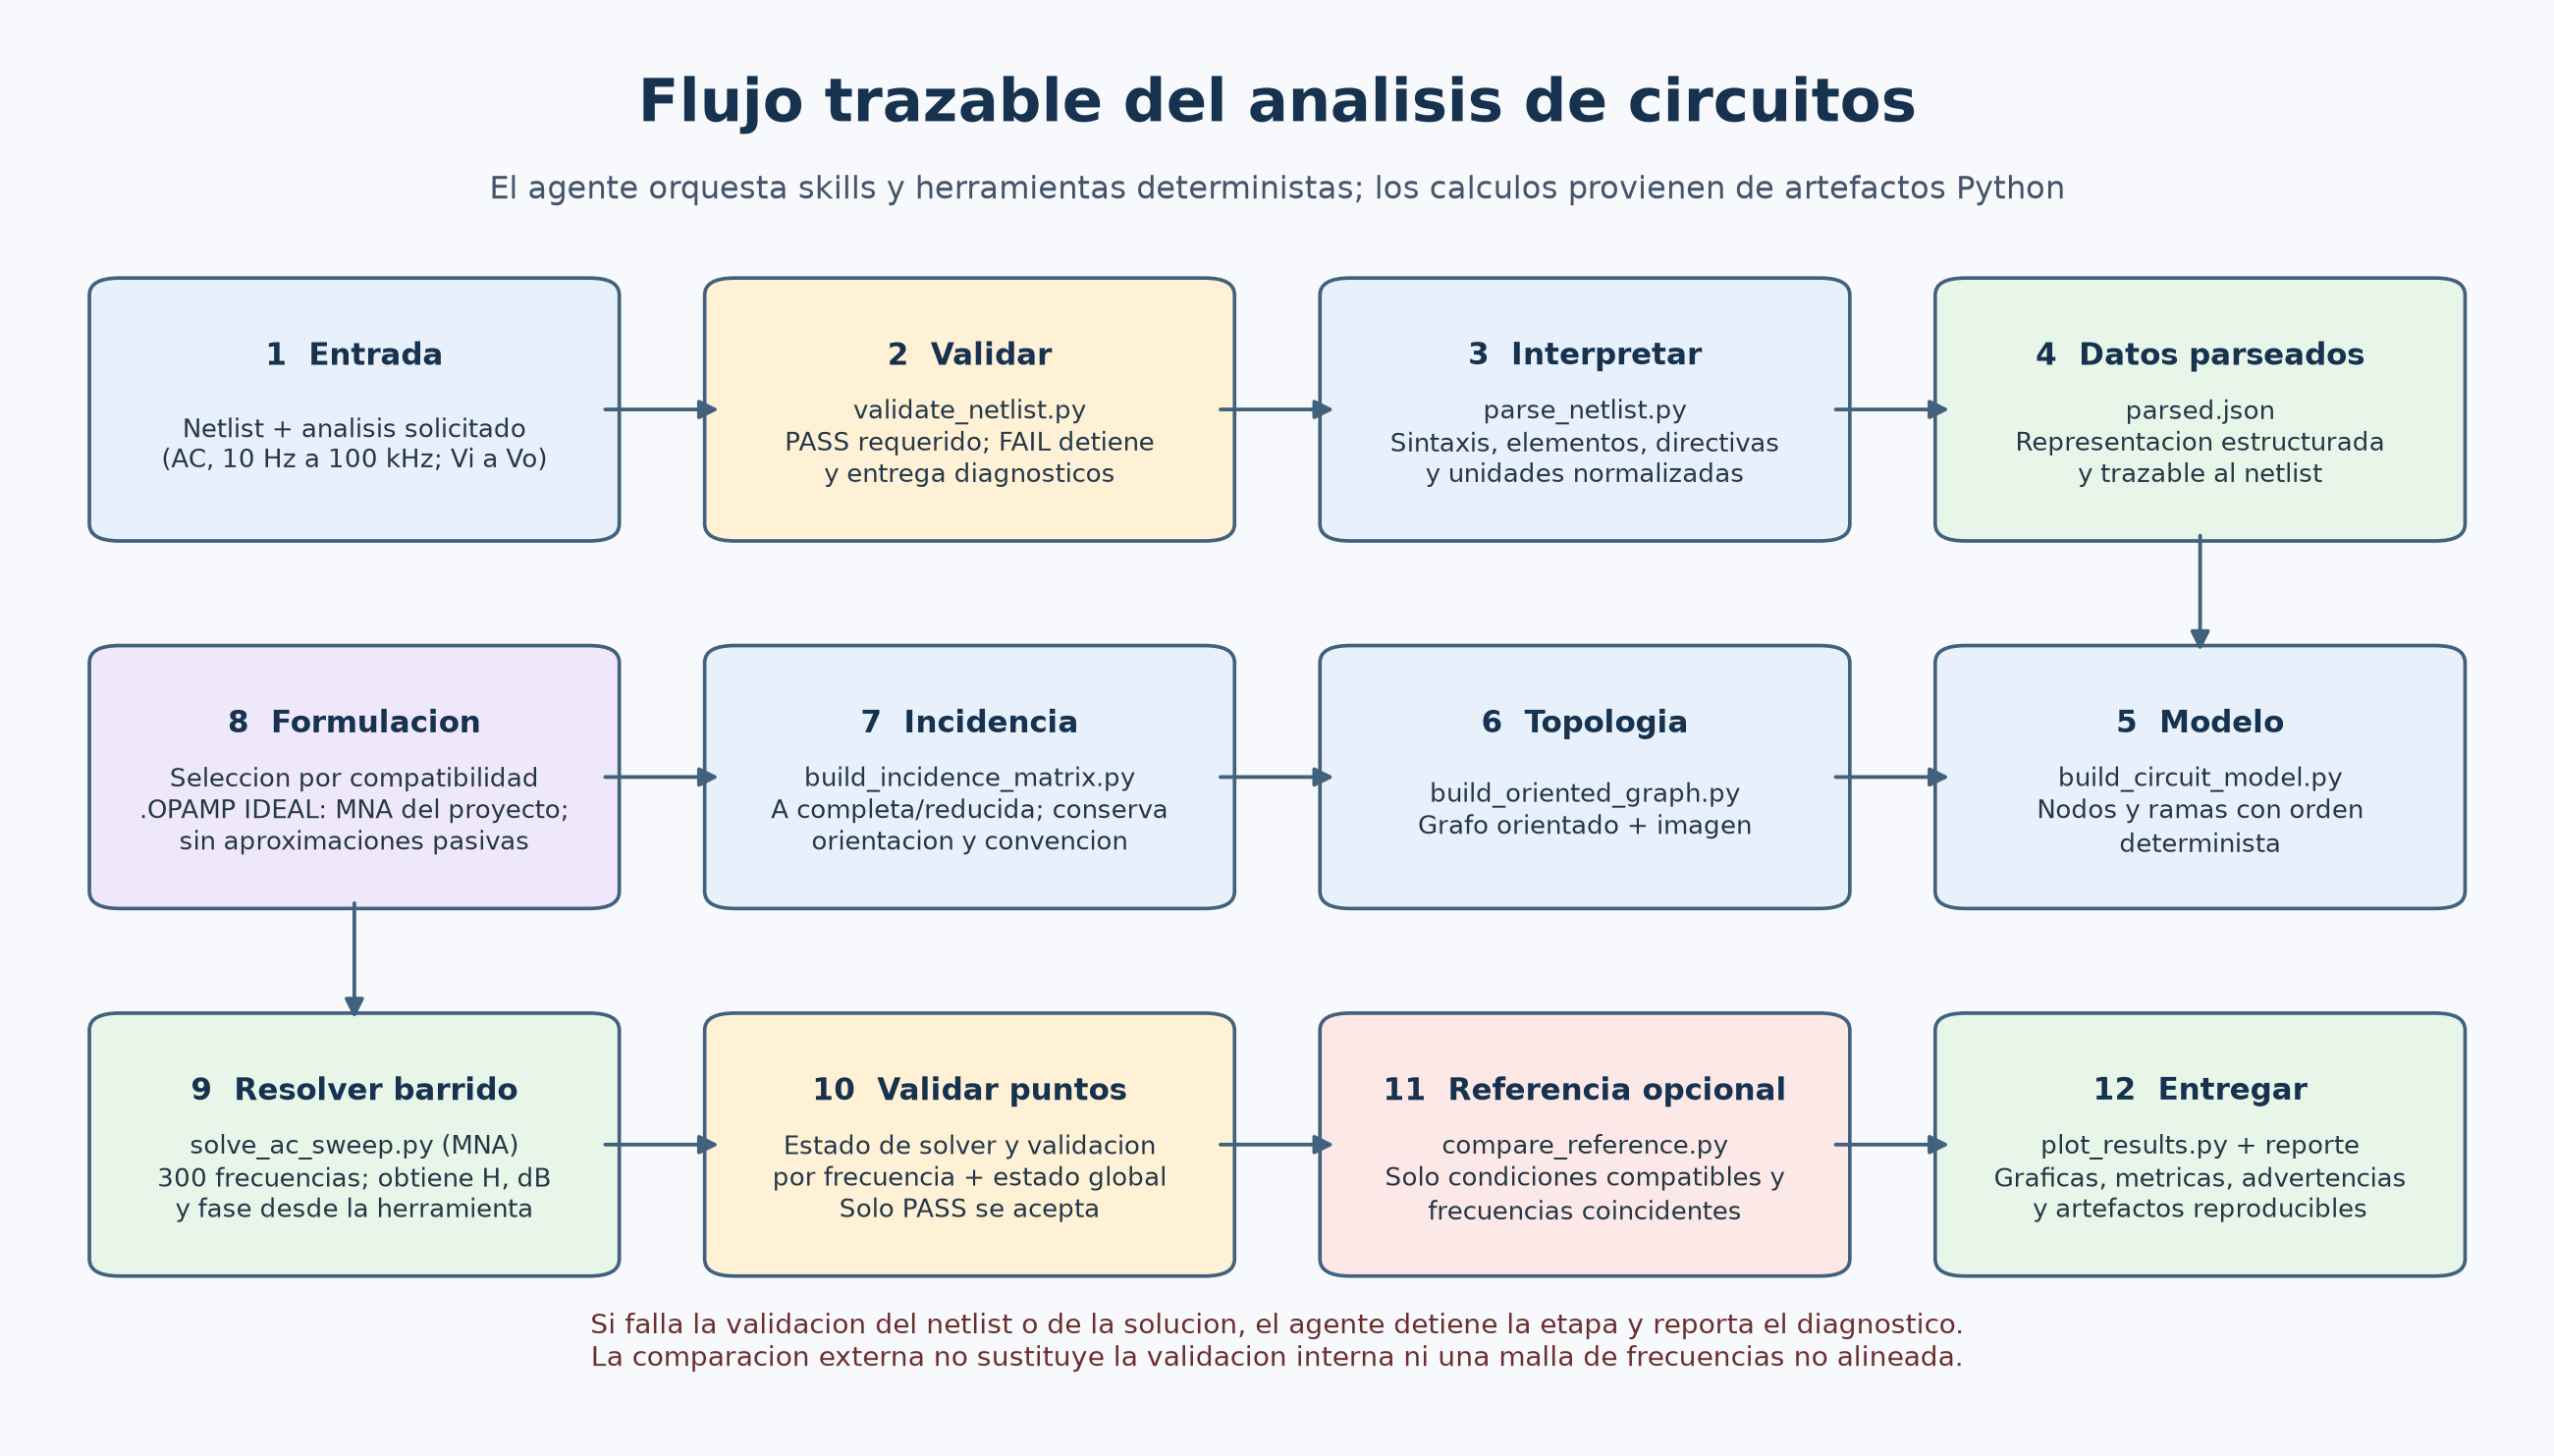
\includegraphics[scale=0.35]{flujo_analisis_agente.png}
\caption{Etapas del agente: validación, construcción del modelo, formulación, resolución, verificación y entrega. Las puertas en FAIL detienen el flujo.}
\end{figure}
\section{Resumen de la bitacora del proyecto}
La siguiente sintesis recoge los hitos y estados consignados en \textit{Bitacora de trabajo -- Proyecto SPICE}. Se resumen evidencias del desarrollo del Agente tipo SPICE.

\begin{table}[H]
\small
\renewcommand{\arraystretch}{1.2}
\begin{tabularx}{\textwidth}{p{1.7cm} p{2.8cm} X}
\toprule
Fecha & Etapa & Trabajo y evidencia registrada \\
\midrule
2026-10-10 & Revision y arquitectura & Auditoria de los diez skills, las seis herramientas iniciales, interfaces, convenciones y pruebas. Se identificaron brechas de validacion, compatibilidad AC/DC y orden determinista; se planifico el desarrollo de herramientas restantes. \\
2026-10-10 & Herramientas y flujo & Desarrollo e integracion de herramientas para modelos constitutivos, Tableau, solver, barrido AC, validacion, comparacion, reportes y graficas. La bitacora registra pruebas de flujos nodal DC, Tableau y AC, junto con correcciones de contratos y datos. \\
2026-11-02 & Reporte y analisis AC & Se documento el ejemplo RC con bundle, reporte Markdown y graficas. Barrido DEC de 41 puntos: \textbf{Satisfactorio}; las pruebas extendidas y la integracion DC tambien se reportaron aprobadas. \\
2026-11-02 & Validacion y stamps & Se implementaron \texttt{validate\_netlist.py} y \texttt{stamp\_elements.py}, integrando validacion como puerta previa y compartiendo modelos de rama. Verificacion registrada: 10/10 pruebas extendidas, integracion DC y flujo AC RC en \textbf{Satisfactorio}. \\
2026-11-02 & Extension MNA para op-amp & Se implemento la directiva educativa \texttt{.OPAMP ... IDEAL} con corriente auxiliar de salida y restriccion de entradas iguales en operacion lineal. Demostracion AC: 61/61 puntos \textbf{Satisfactorio}; pruebas extendidas 15/15 e integracion DC \textbf{Satisfactorio}. No se reporto comparacion SPICE externa para esa demostracion; el modelo no incluye rieles ni saturacion. \\
\bottomrule
\end{tabularx}
\caption{Hitos resumidos de la bitacora y evidencias/limitaciones reportadas.}
\end{table}
\section{Circuito Objetivo (Caso 1)}

El primer caso que se analizó es un filtro activo con Amplificadores operacionales. A continuación se muestra su esquemático y los valores de los elementos.

\begin{figure}[H]
\centering
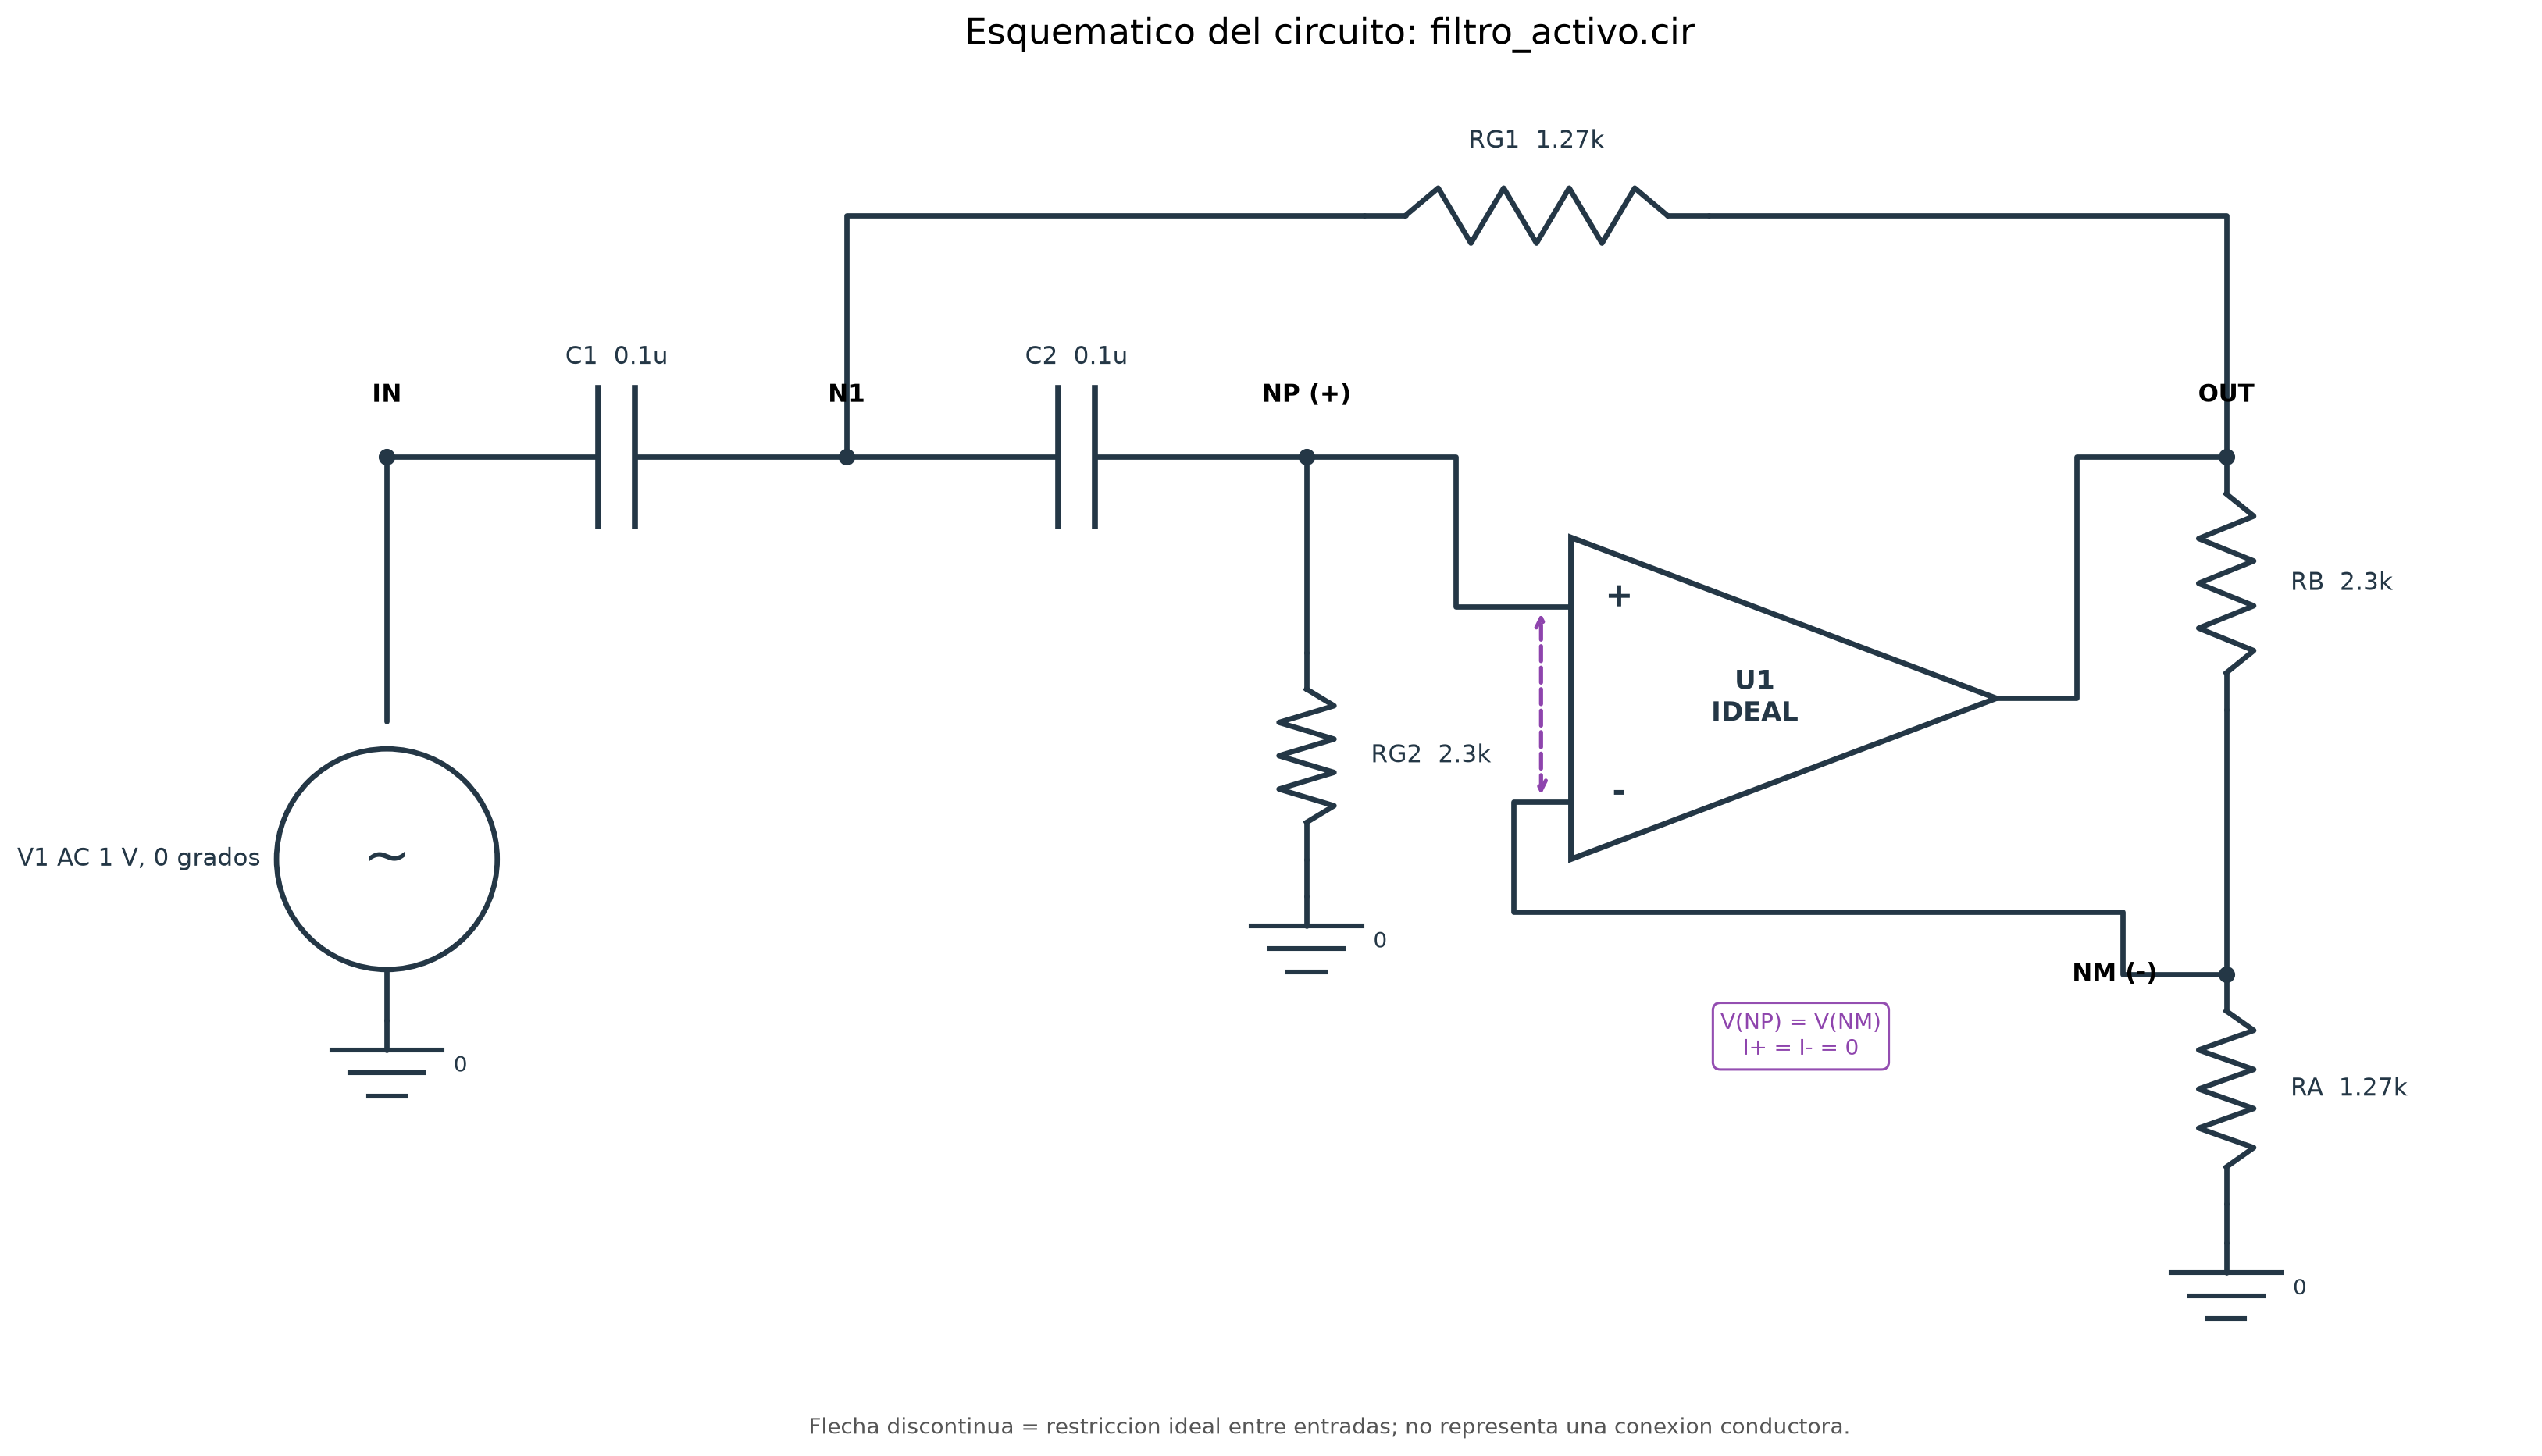
\includegraphics[width=0.8\linewidth]{1_circuito_objetivo_agent/plots/esquematico_filtro_activo.png}
\caption{Esquemático del circuito objetivo.}
\end{figure}

\begin{table}[H]
\centering
\begin{tabular}{ll}
\toprule
Parámetro & Valor \\
\midrule
Frecuencia de inicio & 10 Hz \\
Frecuencia final & 100 kHz \\
Tipo de barrido & Lineal, 300 puntos \\
Fuente AC de entrada & 1 V \\
$C_1$, $C_2$ & 0.1 $\mu$F \\
$R_A$ & 1.27 k$\Omega$ \\
$R_B$ & 2.3 k$\Omega$ \\
$R_G1$ & 1.27 k$\Omega$ \\
$R_G2$ & 2.3 k$\Omega$ \\
Modelo del op-amp & Ideal, extensión MNA del proyecto \\
\bottomrule
\end{tabular}
\caption{Parámetros de simulación del circuito objetivo.}
\end{table}

\subsection{Resultados del analisis en AC del Agente y HSPICE}

La herramienta proporcionó el siguiente análisis de grafos:
\begin{figure}[H]
\centering
\includegraphics[width=0.8\linewidth]{1_circuito_objetivo_agent/plots/graph.png}
\caption{Análisis de grafos del circuito objetivo.}
\end{figure}

Parte del análisis que genera incluye la formulación de la matriz de Tableua. Nota: El agente no pudo formular completamente la matriz de Tableua, la matriz mostrada a continuación no muestra el elemento del OpAmp, de acuerdo con el agente el analisis MNA cubre lo correspondiente al OpAmp.

\begin{figure}[H]
\centering
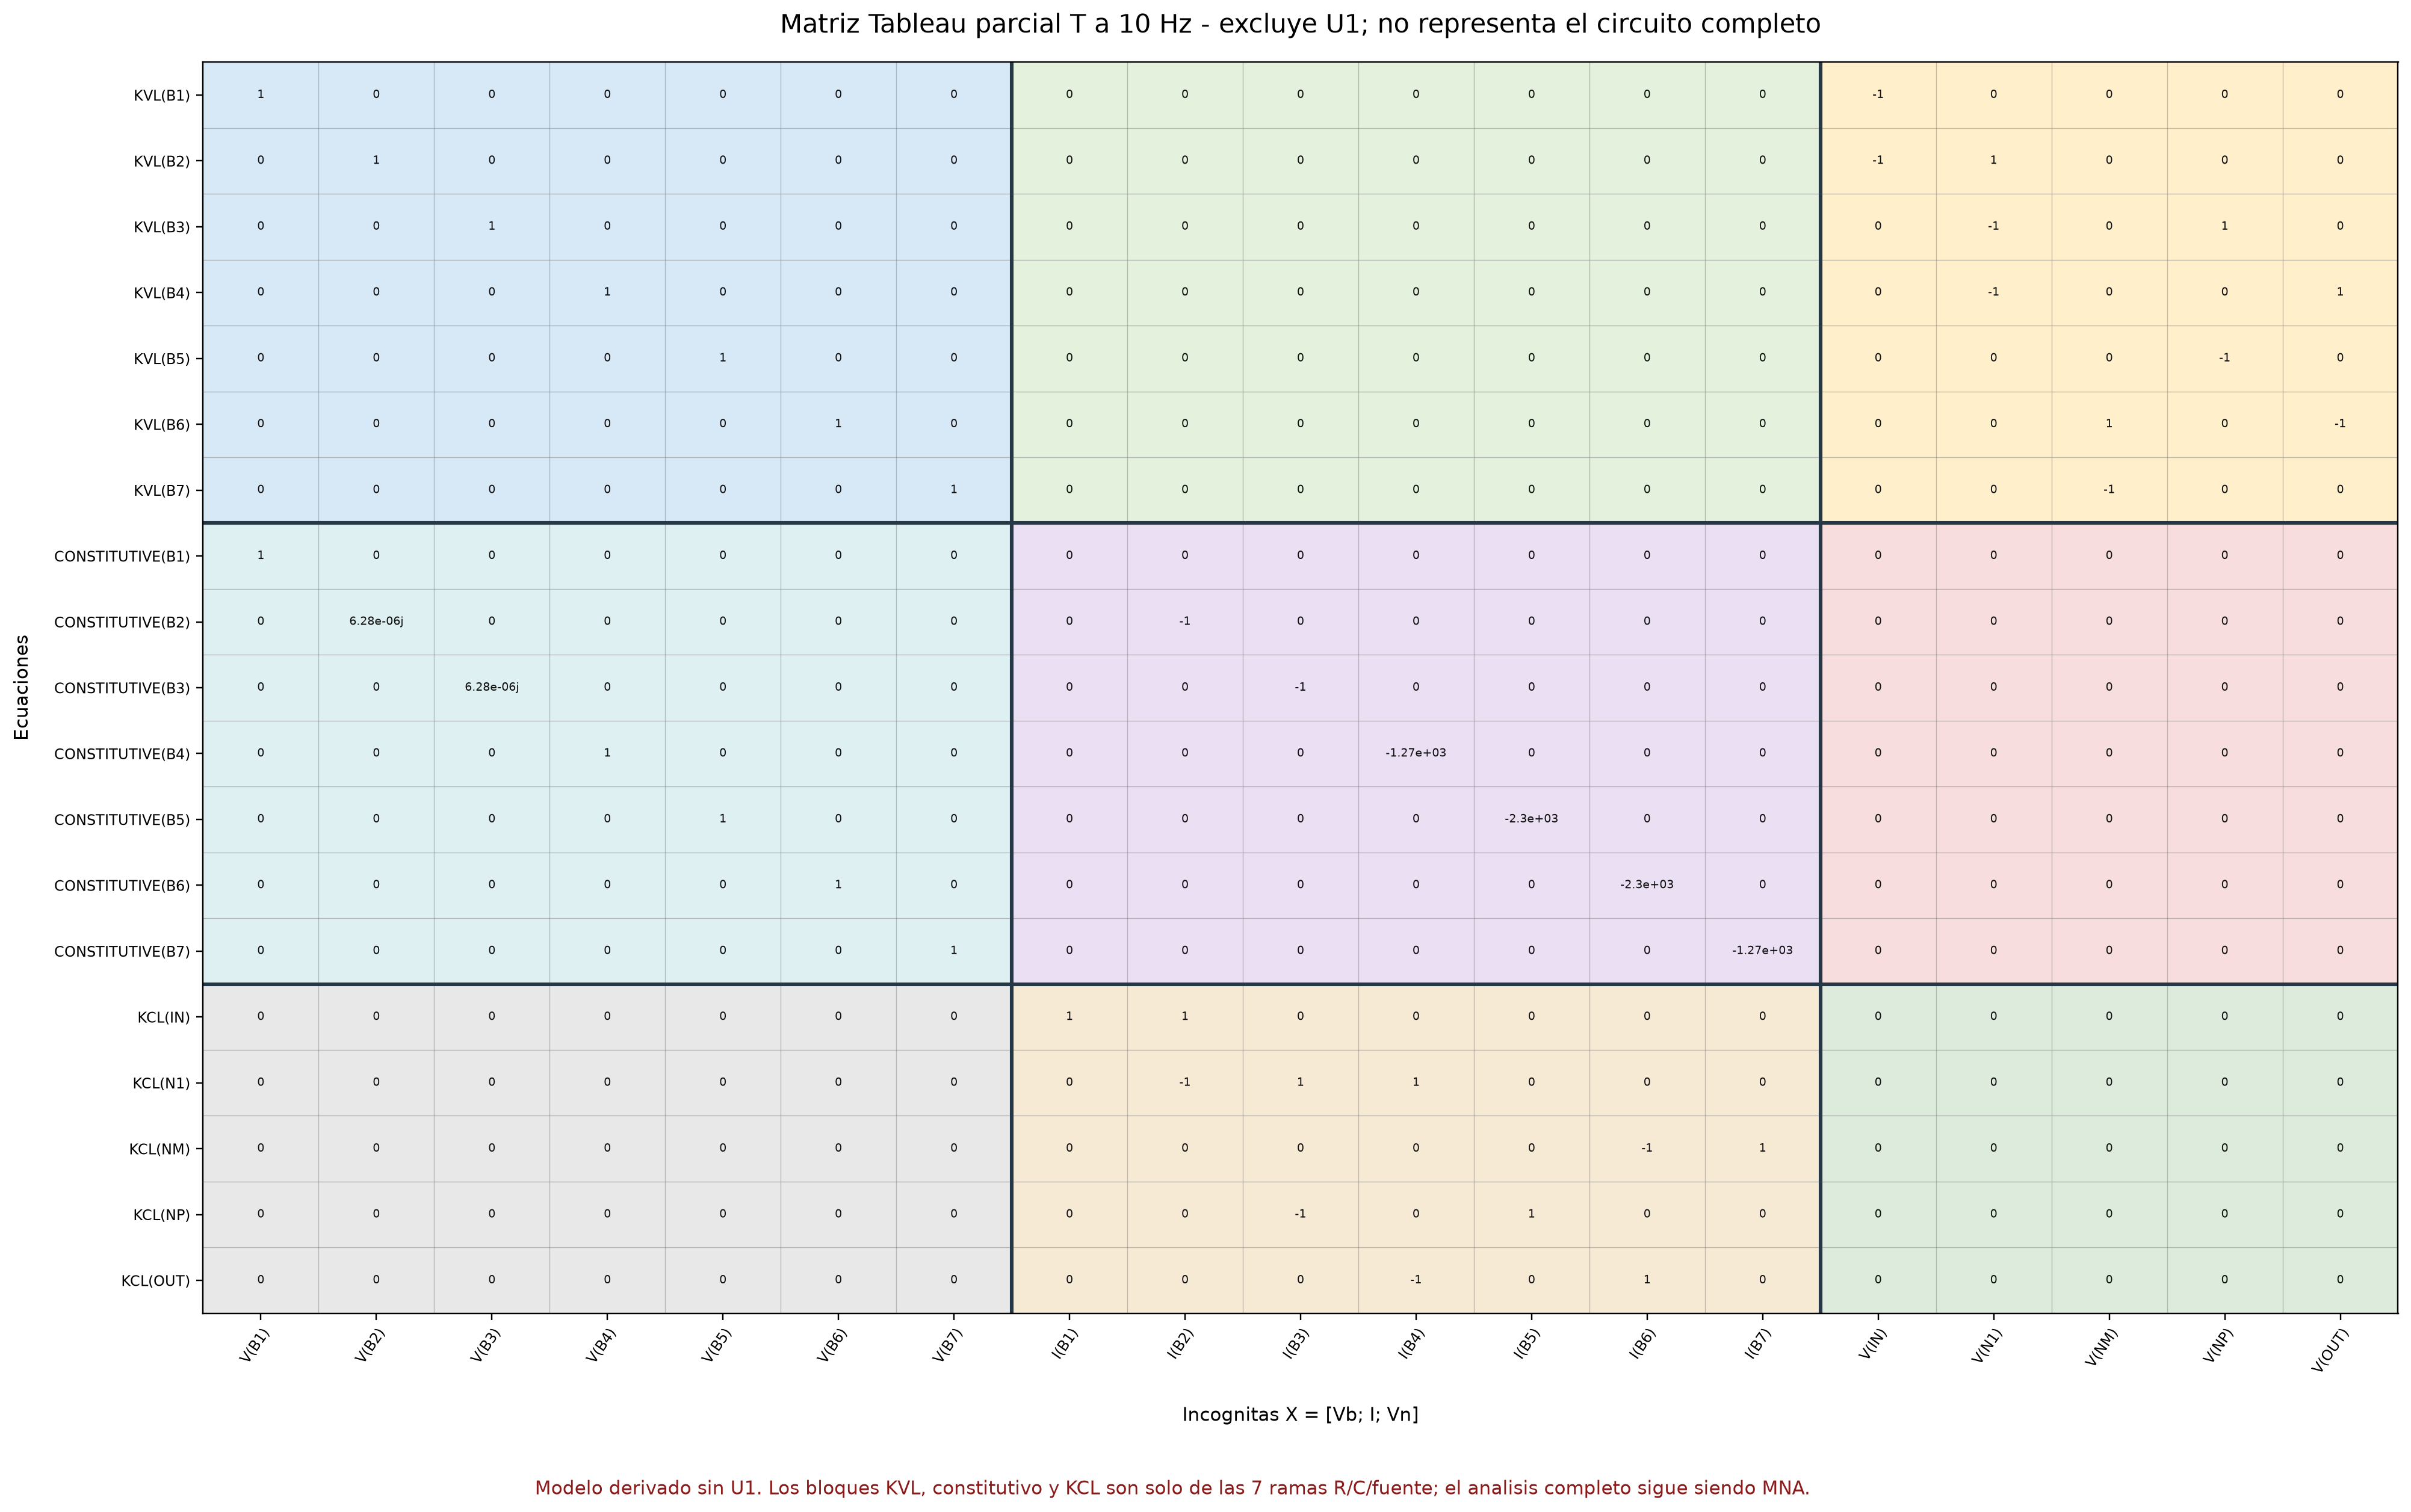
\includegraphics[width=0.8\linewidth]{1_circuito_objetivo_agent/plots/tableau_partial_T_colored_blocks_10Hz.png}
\caption{Matriz de Tableua del circuito objetivo.}
\end{figure}

\begin{figure}[H]
\centering
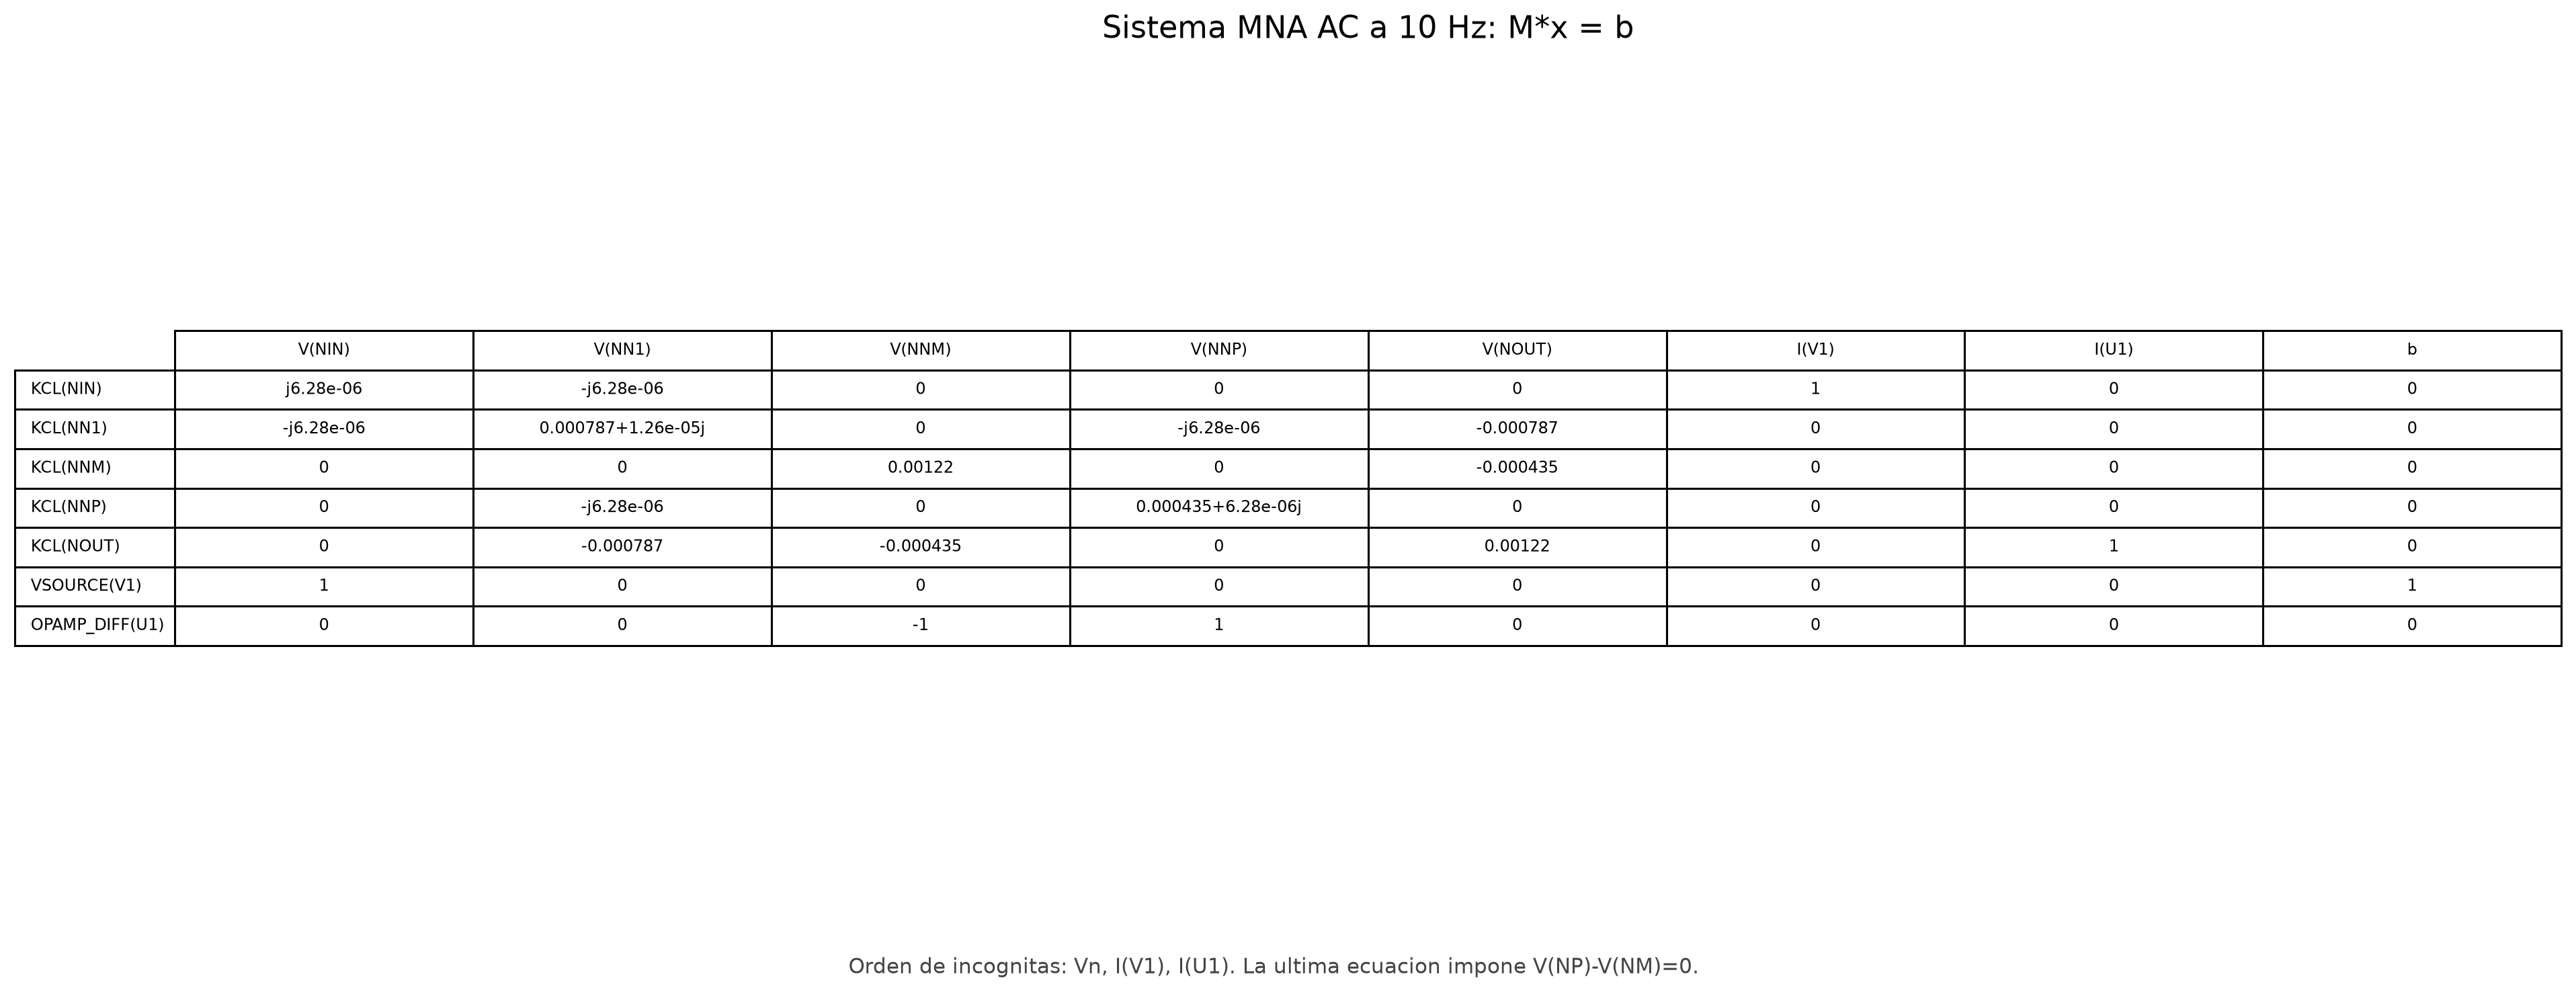
\includegraphics[width=0.95\linewidth]{1_circuito_objetivo_agent/plots/mna_system_10Hz.png}
\caption{Sistema MNA AC completo del circuito a 10 Hz.}
\end{figure}

La herramienta del proyecto reportó un estado general \textbf{Satisfactorio} para el barrido entero. La transferencia se evaluó como $V(NOUT)/V(NIN)$, con validación de cada punto y estado global de la ejecución correcto.

\begin{table}[H]
\centering
\begin{tabular}{lrrr}
\toprule
Punto & Frecuencia (Hz) & $|H(j\omega)|$ & Fase ($^\circ$) \\
\midrule
Inicio & 10 & 0.0003241778 & -179.4148 \\
Punto de máximo local & 1347.6589 & 3.3482009 & -51.5098 \\
Fin & 100000 & 2.8111572 & -0.5074 \\
\bottomrule
\end{tabular}
\caption{Valores representativos del análisis AC del agente SPICE educativo.}
\end{table}

\begin{figure}[H]
\centering
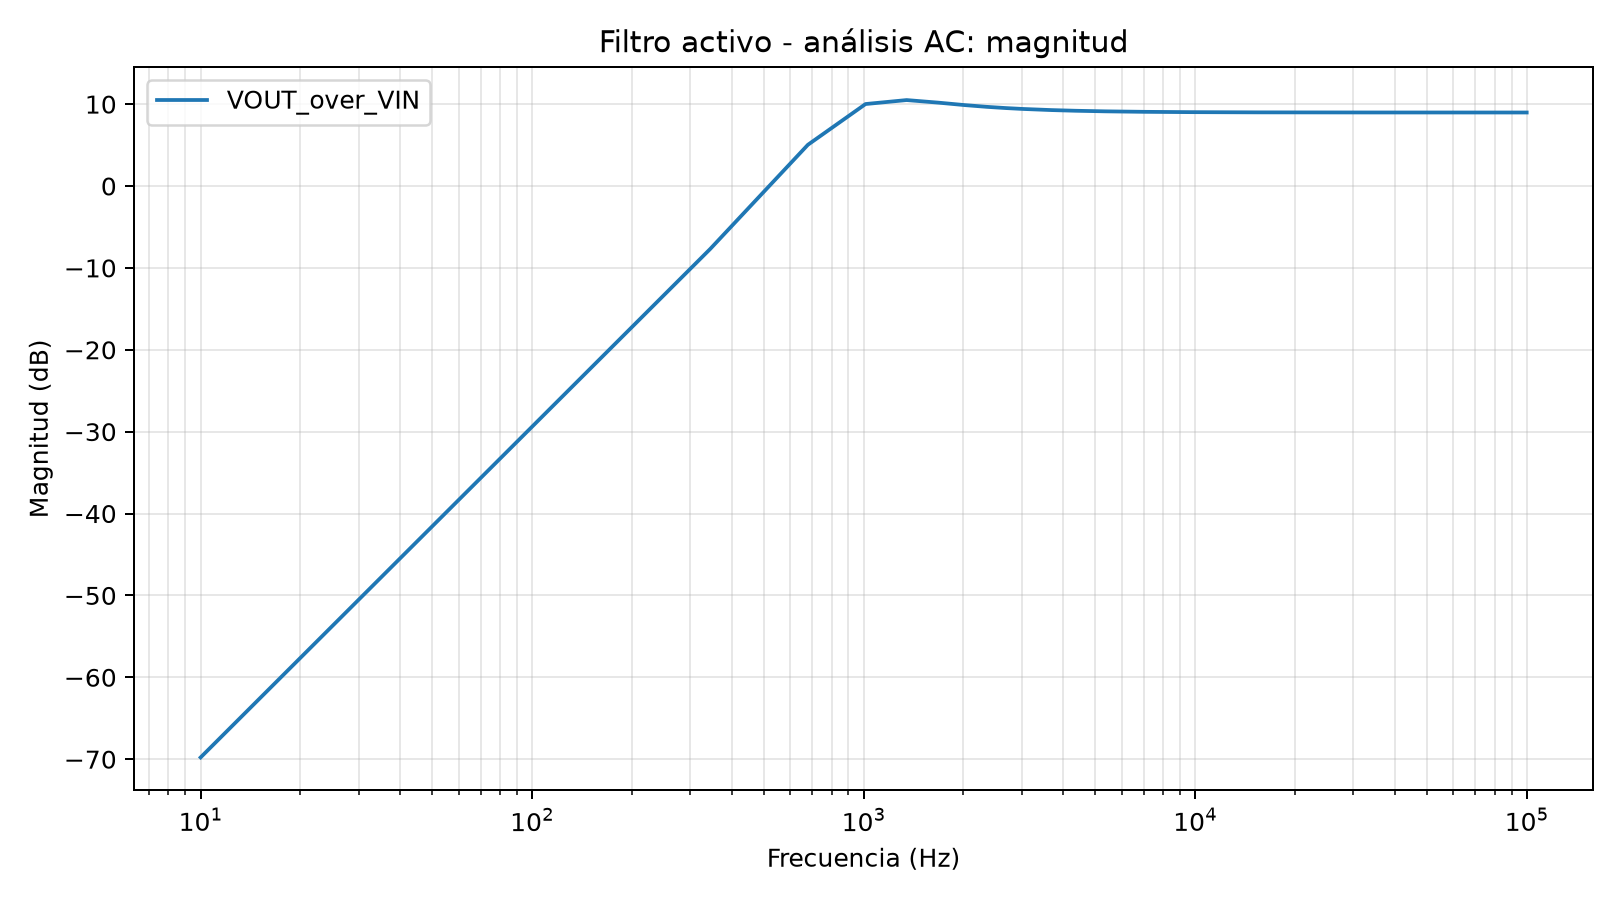
\includegraphics[width=0.8\linewidth]{1_circuito_objetivo_agent/plots/magnitude.png}
\caption{Gráfica de Magnitud en dB de la función de transferencia $H(w)$ obtenida por el agente.}
\end{figure}

\begin{figure}[H]
\centering
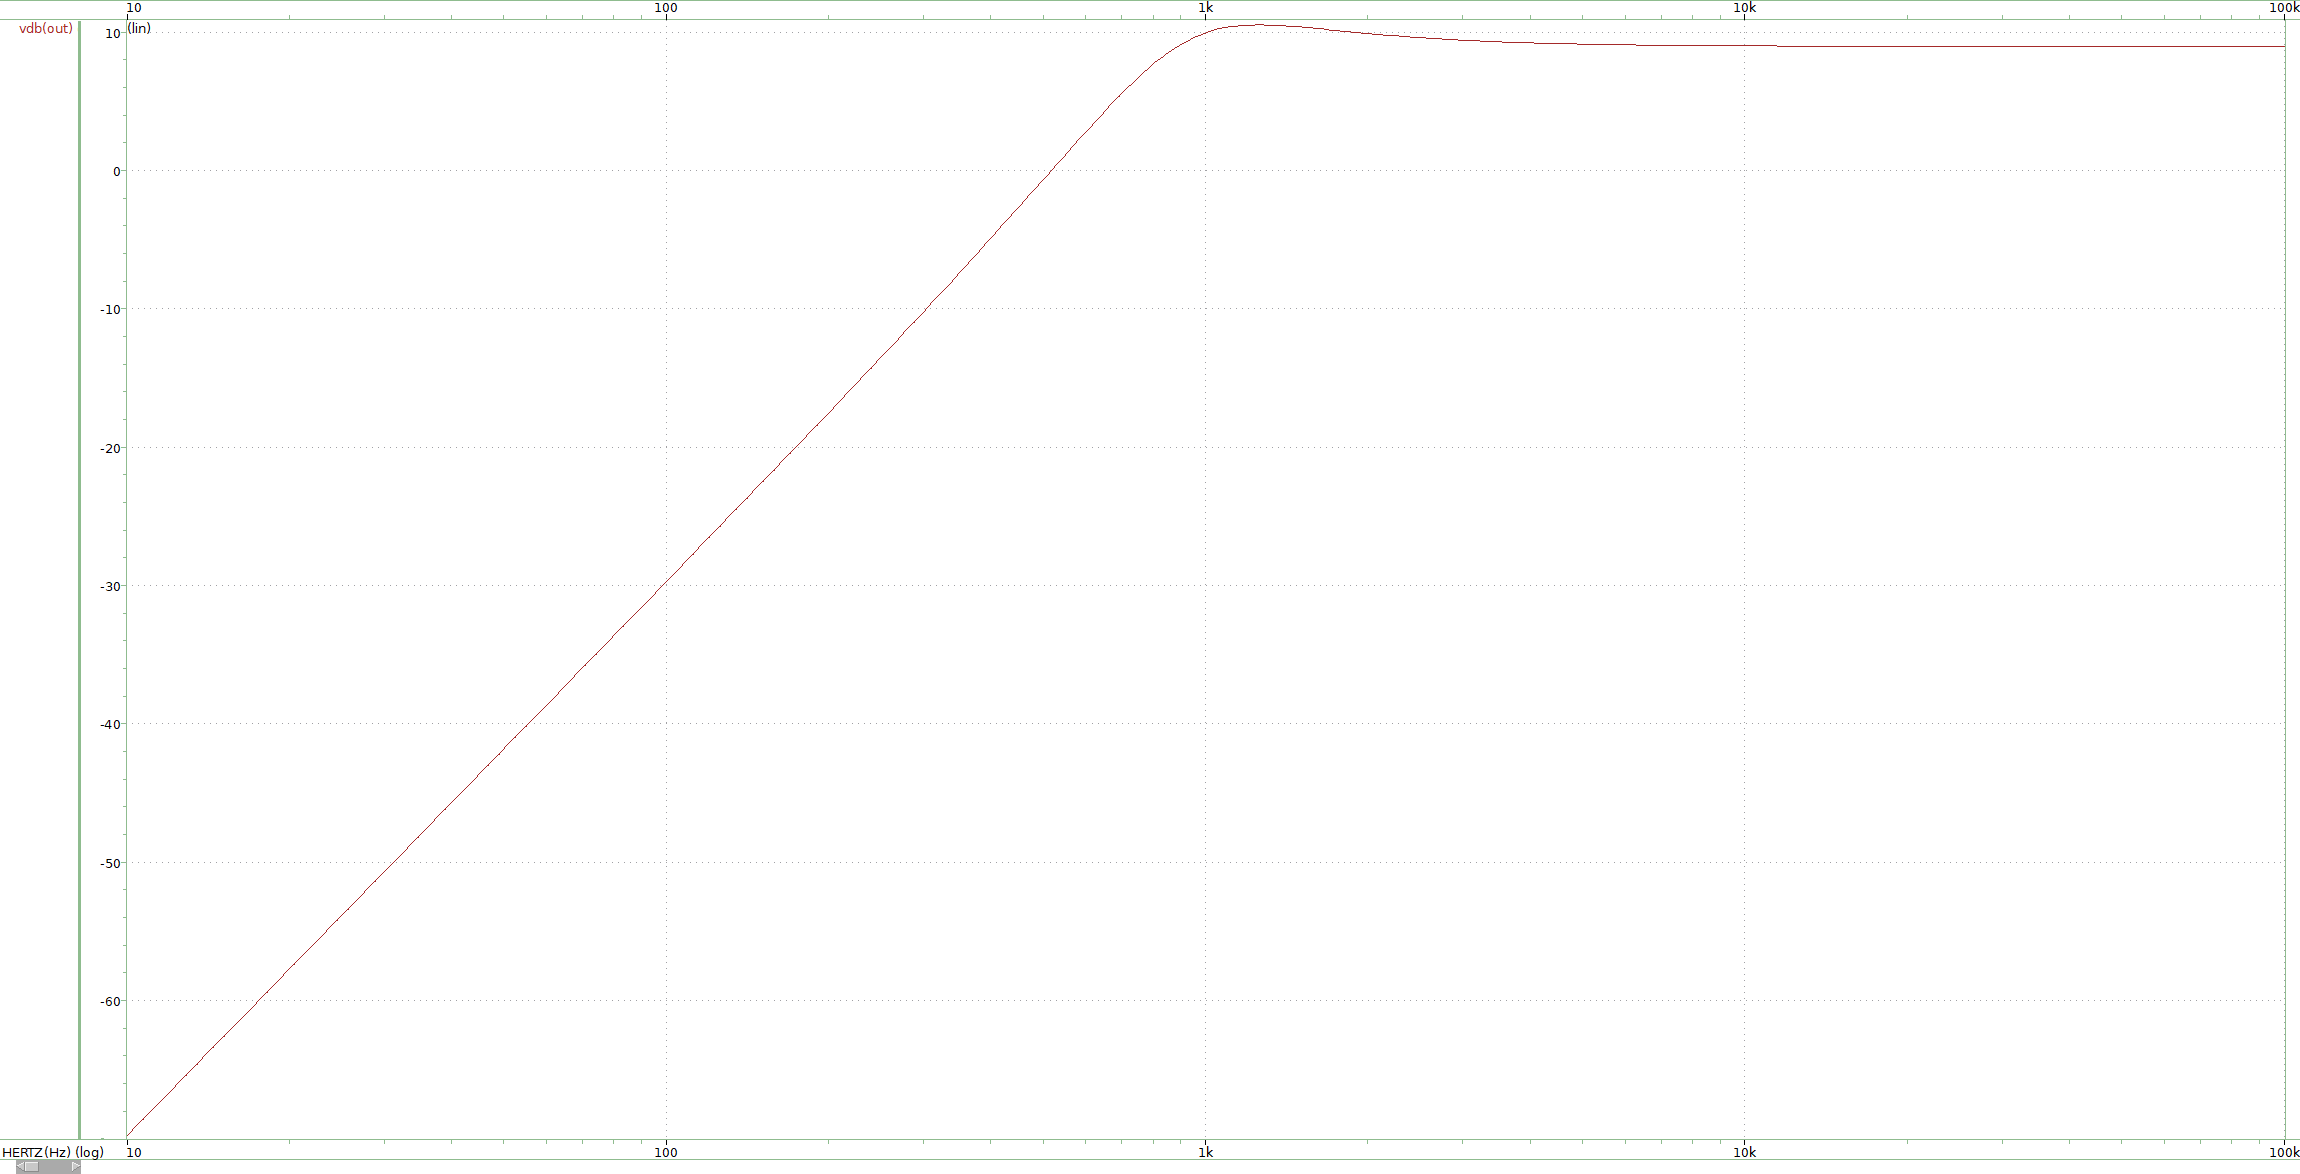
\includegraphics[width=0.8\linewidth]{1_circuito_objetivo_HSPICE/magnitude_dB_hspice.png}
\caption{Gráfica de Magnitud en dB de la función de transferencia $H(w)$ obtenida por HSPICE.}
\end{figure}

\begin{figure}[H]
\centering
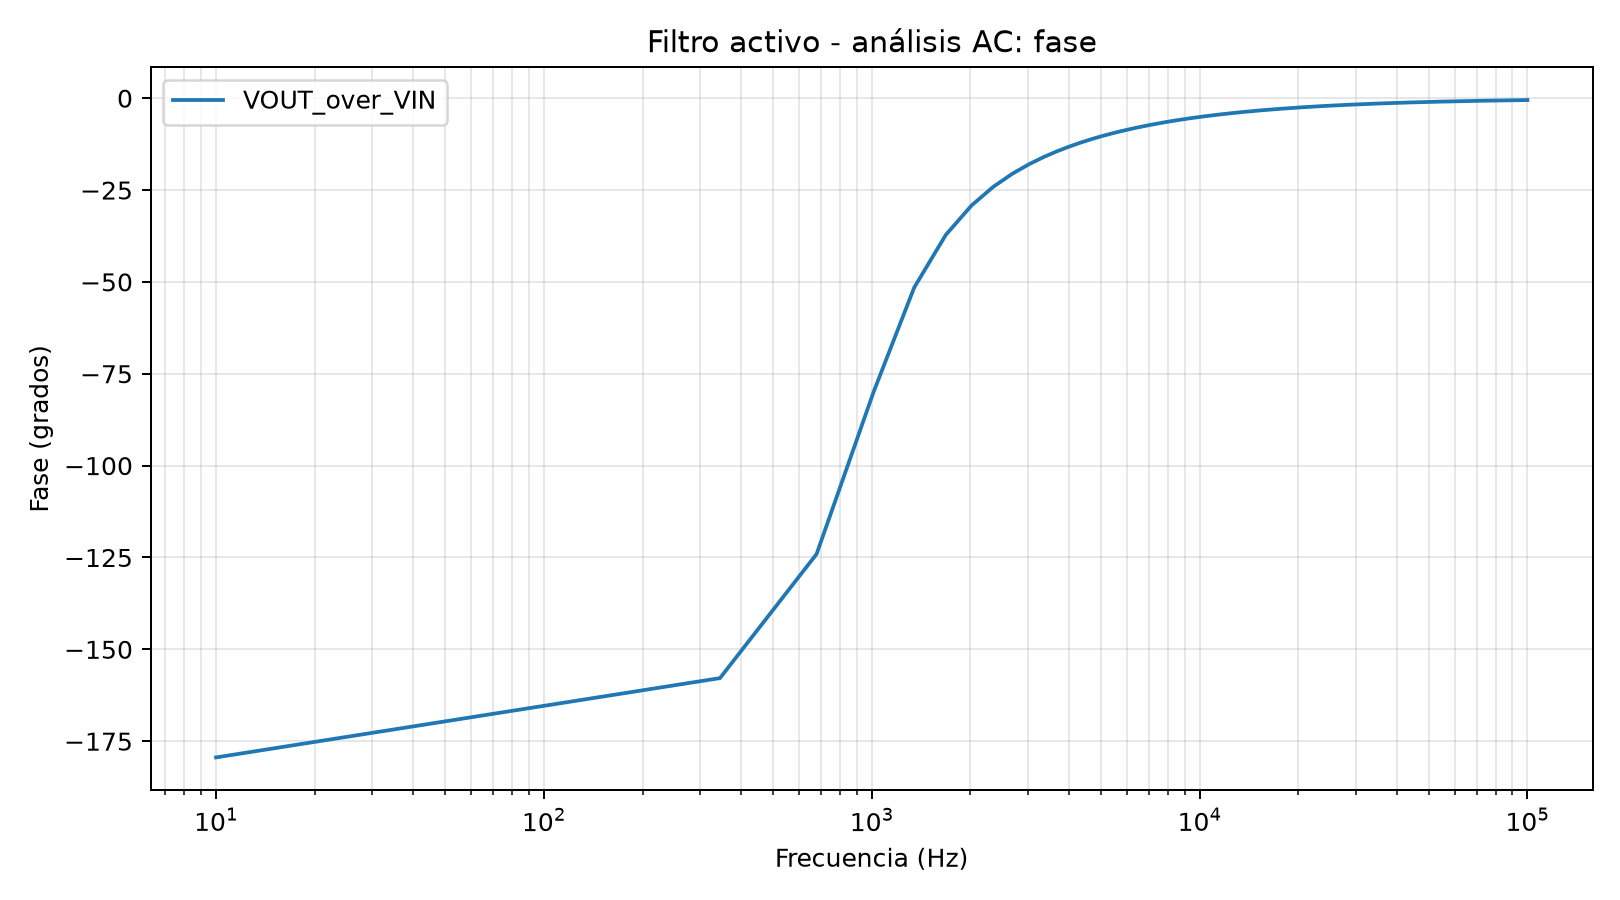
\includegraphics[width=0.8\linewidth]{1_circuito_objetivo_agent/plots/phase.png}
\caption{Gráfica de Fase de la función de transferencia $H(w)$ obtenida por el agente.}
\end{figure}

\begin{figure}[H]
\centering
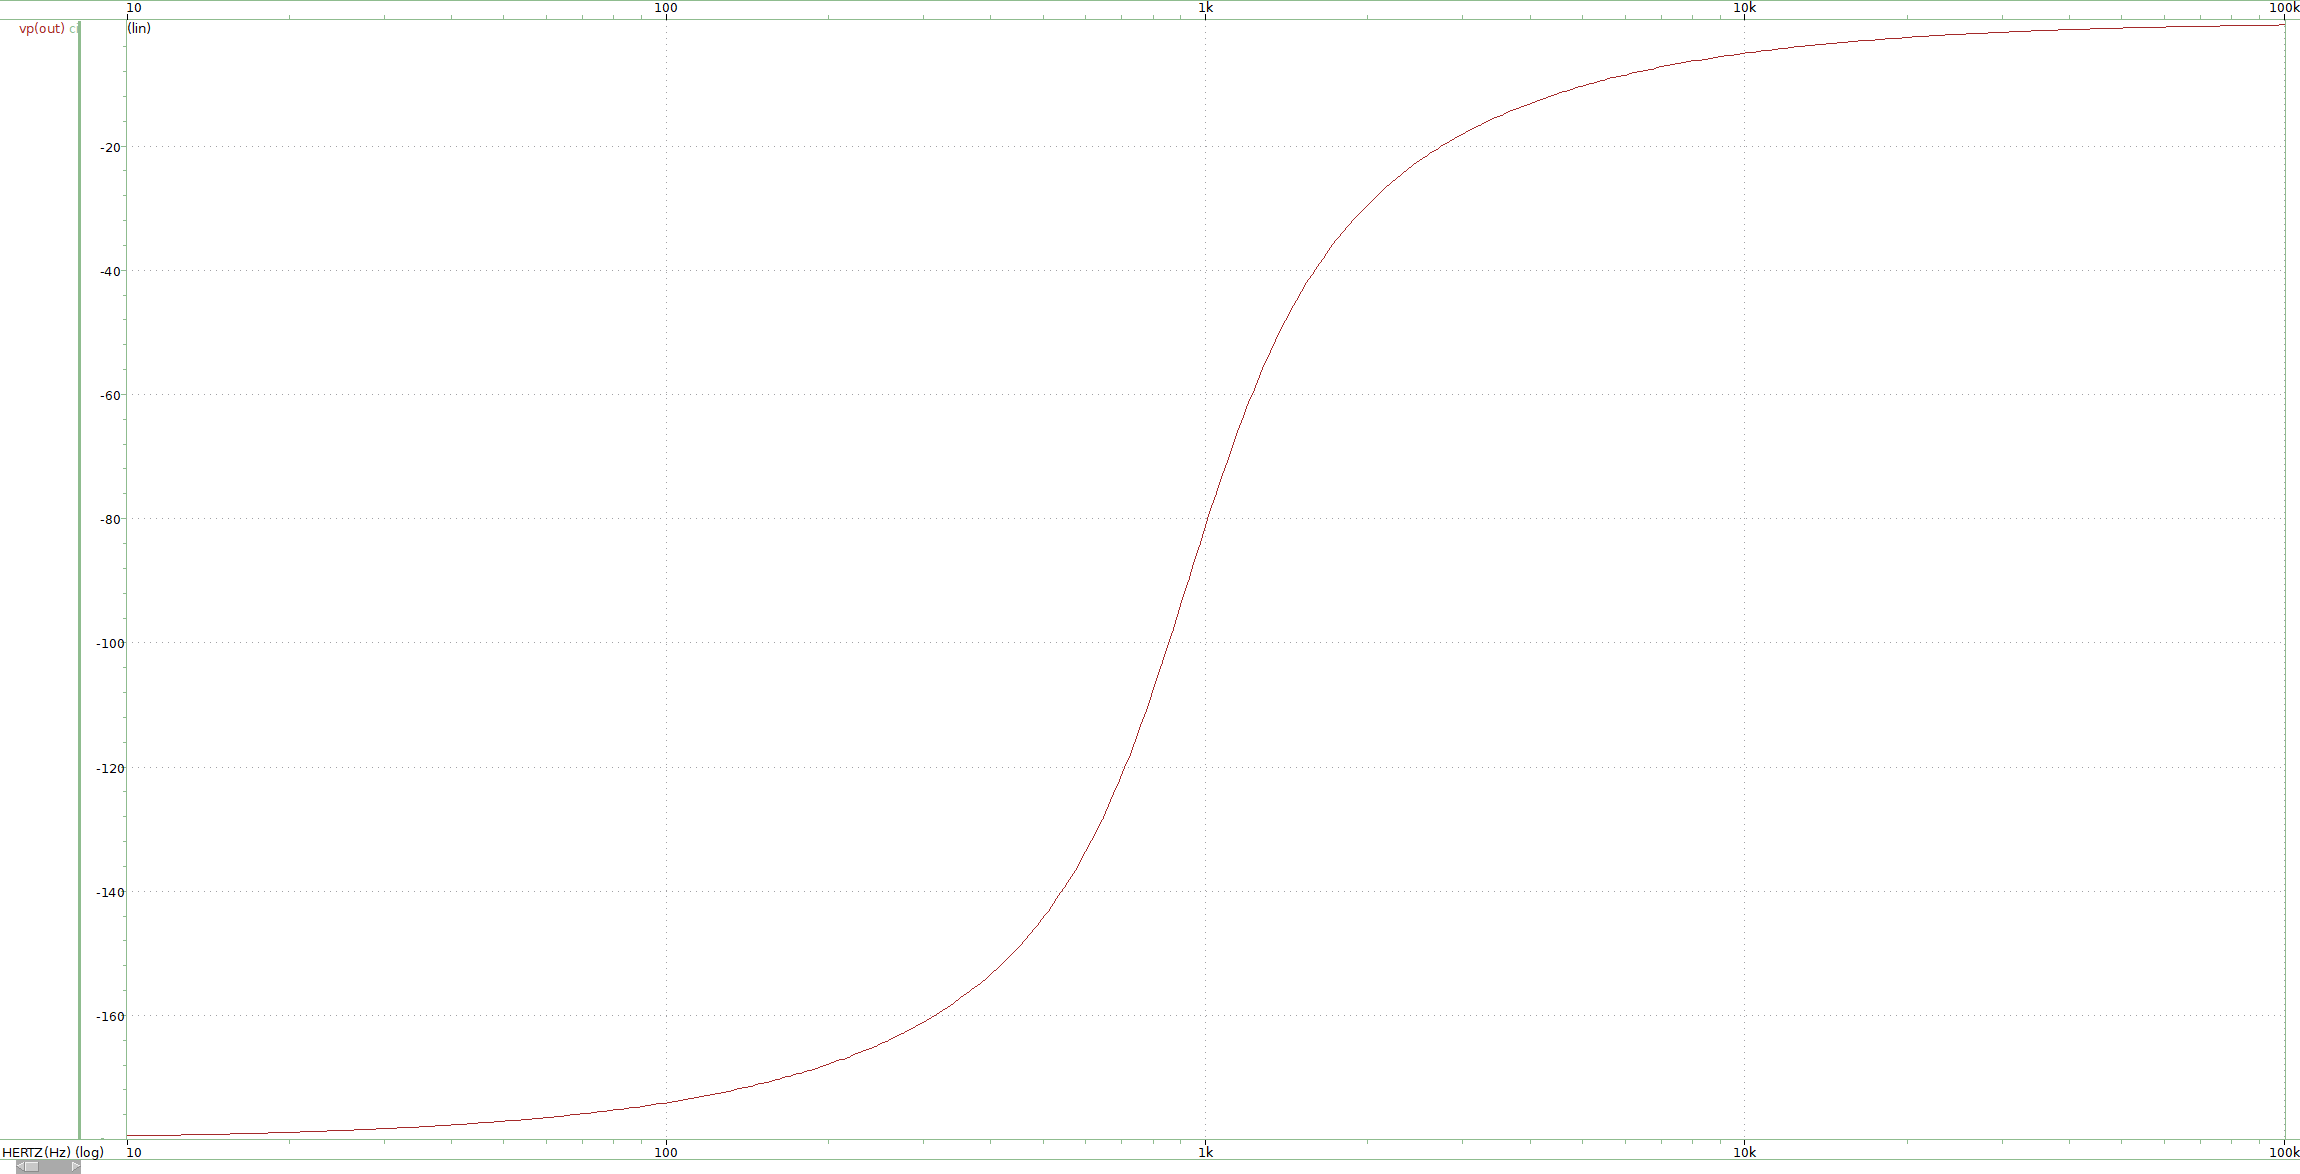
\includegraphics[width=0.8\linewidth]{1_circuito_objetivo_HSPICE/phase_hspice.png}
\caption{Gráfica de Fase de la función de transferencia $H(w)$ obtenida por HSPICE.}
\end{figure}

\begin{figure}[H]
\centering
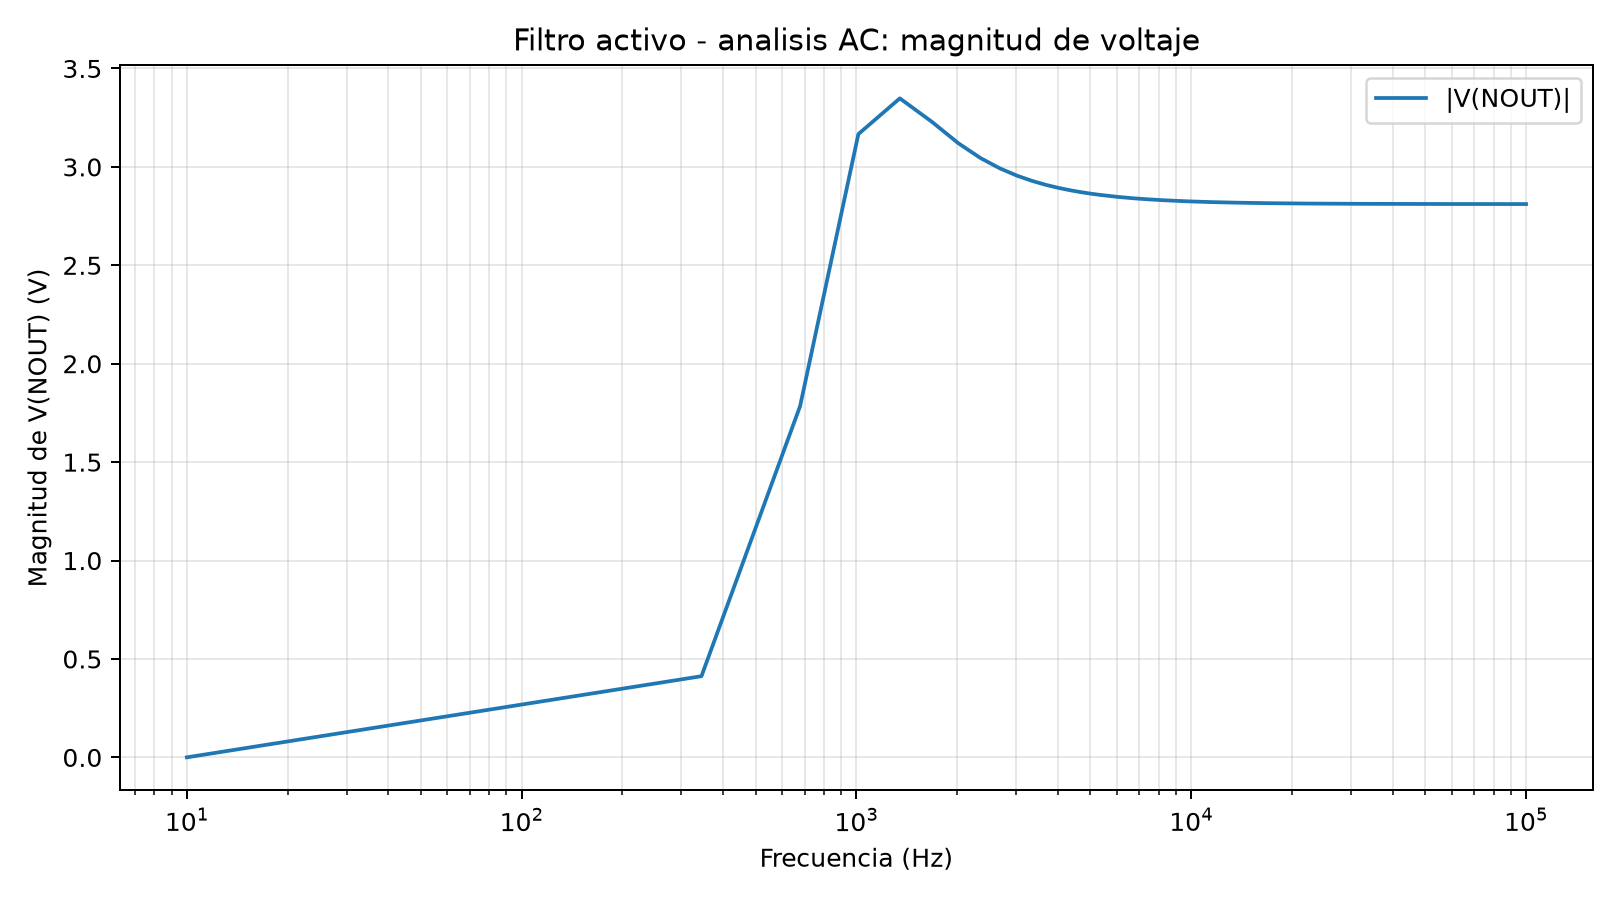
\includegraphics[width=0.75\linewidth]{1_circuito_objetivo_agent/plots/magnitude_voltage.png}
\caption{Gráfica de Magnitud en Voltaje de $V\_OUT$ obtenida por el agente.}
\end{figure}

\begin{figure}[H]
\centering
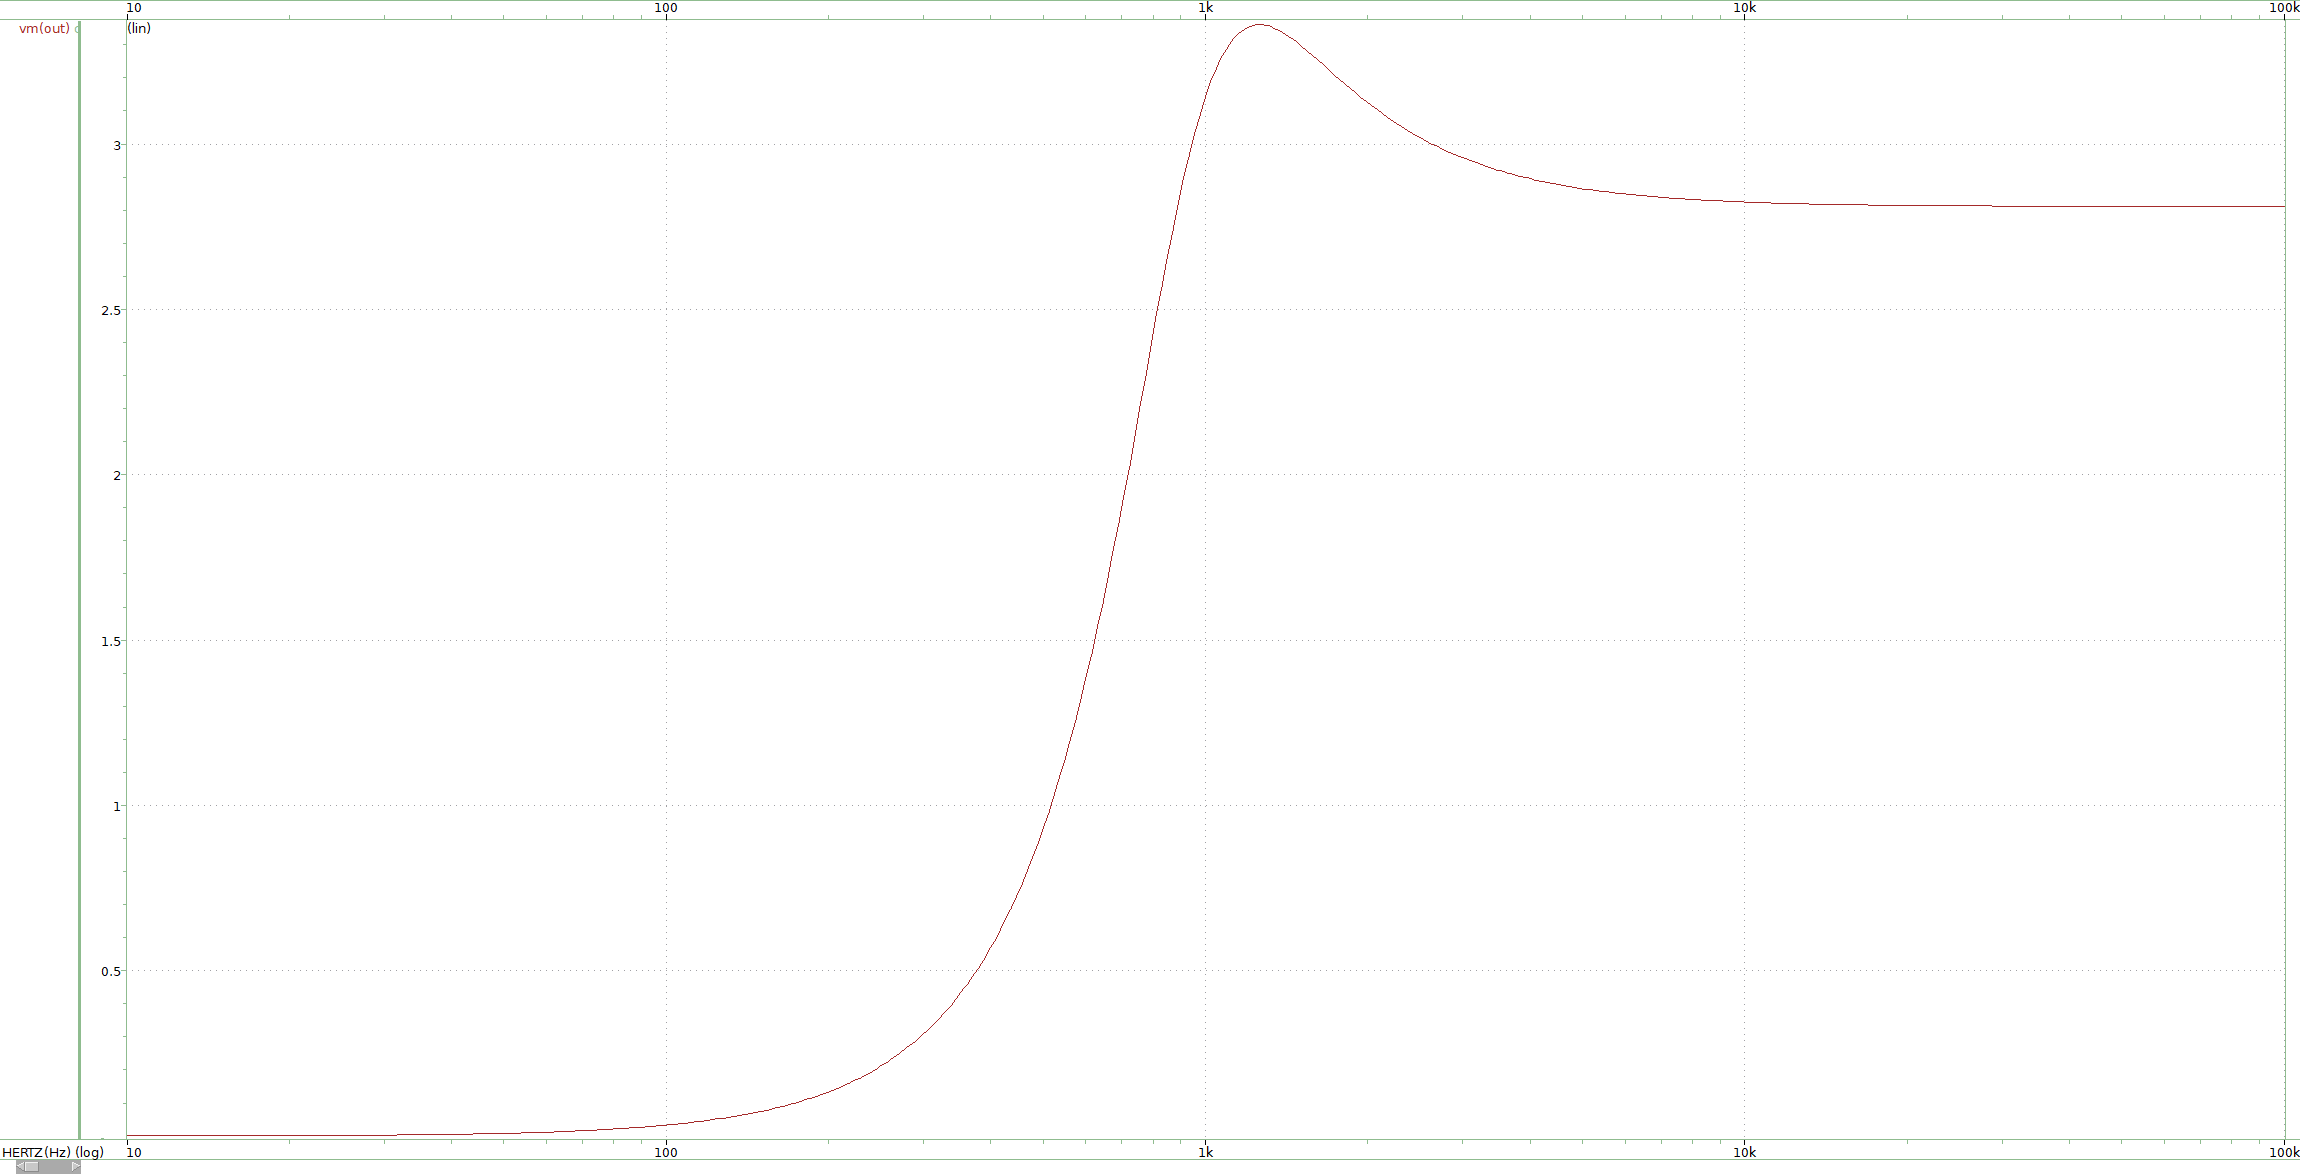
\includegraphics[width=0.75\linewidth]{1_circuito_objetivo_HSPICE/magnitude_voltage_hspice.png}
\caption{Gráfica de Magnitud en Voltaje de $V\_OUT$ obtenida por HSPICE.}
\end{figure}


\subsection{Comparaci\'on con HSPICE}
La comparaci\'on se hizo usando los resultados MNA de \texttt{ac\_results.json} y el listado externo \texttt{circuito\_objectivo\_hspice.lis} (HSPICE V-2023.12-SP2-1). El listado contiene 401 puntos del barrido HSPICE; la ejecuci\'on del agente contiene 300 puntos lineales entre 10 Hz y 100 kHz. La herramienta \texttt{compare\_reference.py} compar\'o \'unicamente las dos frecuencias exactamente coincidentes, 10 Hz y 100 kHz, sin interpolaci\'on. La comparaci\'on usa la transferencia compleja $H(w)$; en los artefactos, el nombre de la referencia \texttt{Vi\_to\_Vo} corresponde al observable \texttt{VOUT\_over\_VIN} del agente.

La comparaci\'on se ejecut\'o con tolerancias absoluta $10^{-6}$ y relativa $2\times10^{-5}$. Los errores de la tabla y los estados proceden de \texttt{compare\_reference.json}; no se calcularon a partir de las gr\'aficas.

\begin{table}[H]
\centering
\begin{tabular}{lccc}
\toprule
Frecuencia & Valor de $H(w)$ del Agente & Valor de $H(w)$ de HSPICE \\
\midrule
10 Hz
& $-3.24160856\times10^{-4} - 3.31084291\times10^{-6}i$
& $-3.24160891\times10^{-4} - 3.31098646\times10^{-6}i$
 \\

100 kHz
& $2.8110469 - 0.0248967i$
& $2.8110897 - 0.0248971i$ \\
\bottomrule
\end{tabular}
\caption{Comparación de la transferencia compleja en los dos puntos con frecuencia exactamente coincidente.}
\end{table}

\begin{table}[H]
\centering
\begin{tabular}{lccccc}
\toprule
Frecuencia & Error absoluto & Error relativo & Estado \\
\midrule
10 Hz
& $1.4771\times10^{-10}$
& $4.5563\times10^{-7}$
& \textbf{PASS} \\

100 kHz
& $4.2845\times10^{-5}$
& $1.5241\times10^{-5}$
& \textbf{PASS} \\
\bottomrule
\end{tabular}


\caption{Comparación de la transferencia compleja en los dos puntos con frecuencia exactamente coincidente.}
\end{table}


El resultado global de la herramienta fue \textbf{Satisfactorio}, dentro de las tolerancias indicadas. La comparaci\'on es limitada: el netlist MNA del agente implementa el op-amp ideal del proyecto, mientras que el deck HSPICE asociado al listado aproxima U1 con una fuente dependiente de ganancia finita $10^9$.%(Caso 1)
\section{Circuito objetivo con valores modificados (Caso 2)}

\subsection{Parámetros y método}
El circuito conserva la topología del filtro activo del Caso 1 y modifica sus componentes. La fuente de entrada es de 10 V AC con fase de $0^\circ$. El análisis se resolvió mediante el modelo MNA lineal del op-amp ideal implementado por el proyecto. El modelo impone corrientes de entrada nulas y $V(NP)=V(NM)$; no representa saturación ni límites de alimentación.

\begin{table}[H]
\centering
\begin{tabular}{ll}
\toprule
Parámetro & Valor \\
\midrule
Frecuencia de inicio y final & 10 Hz y 100 kHz \\
Tipo de barrido & Lineal, 300 puntos \\
Fuente $V_1$ & 10 V AC, $0^\circ$ \\
$C_1$, $C_2$ & 0.50 $\mu$F cada uno \\
$R_{G1}$, $R_A$ & 3 k$\Omega$ cada uno \\
$R_{G2}$, $R_B$ & 1.5 k$\Omega$ cada uno \\
Op-amp & Ideal lineal, formulación MNA del proyecto \\
\bottomrule
\end{tabular}
\caption{Parámetros del circuito objetivo modificado.}
\end{table}

\begin{figure}[H]
\centering
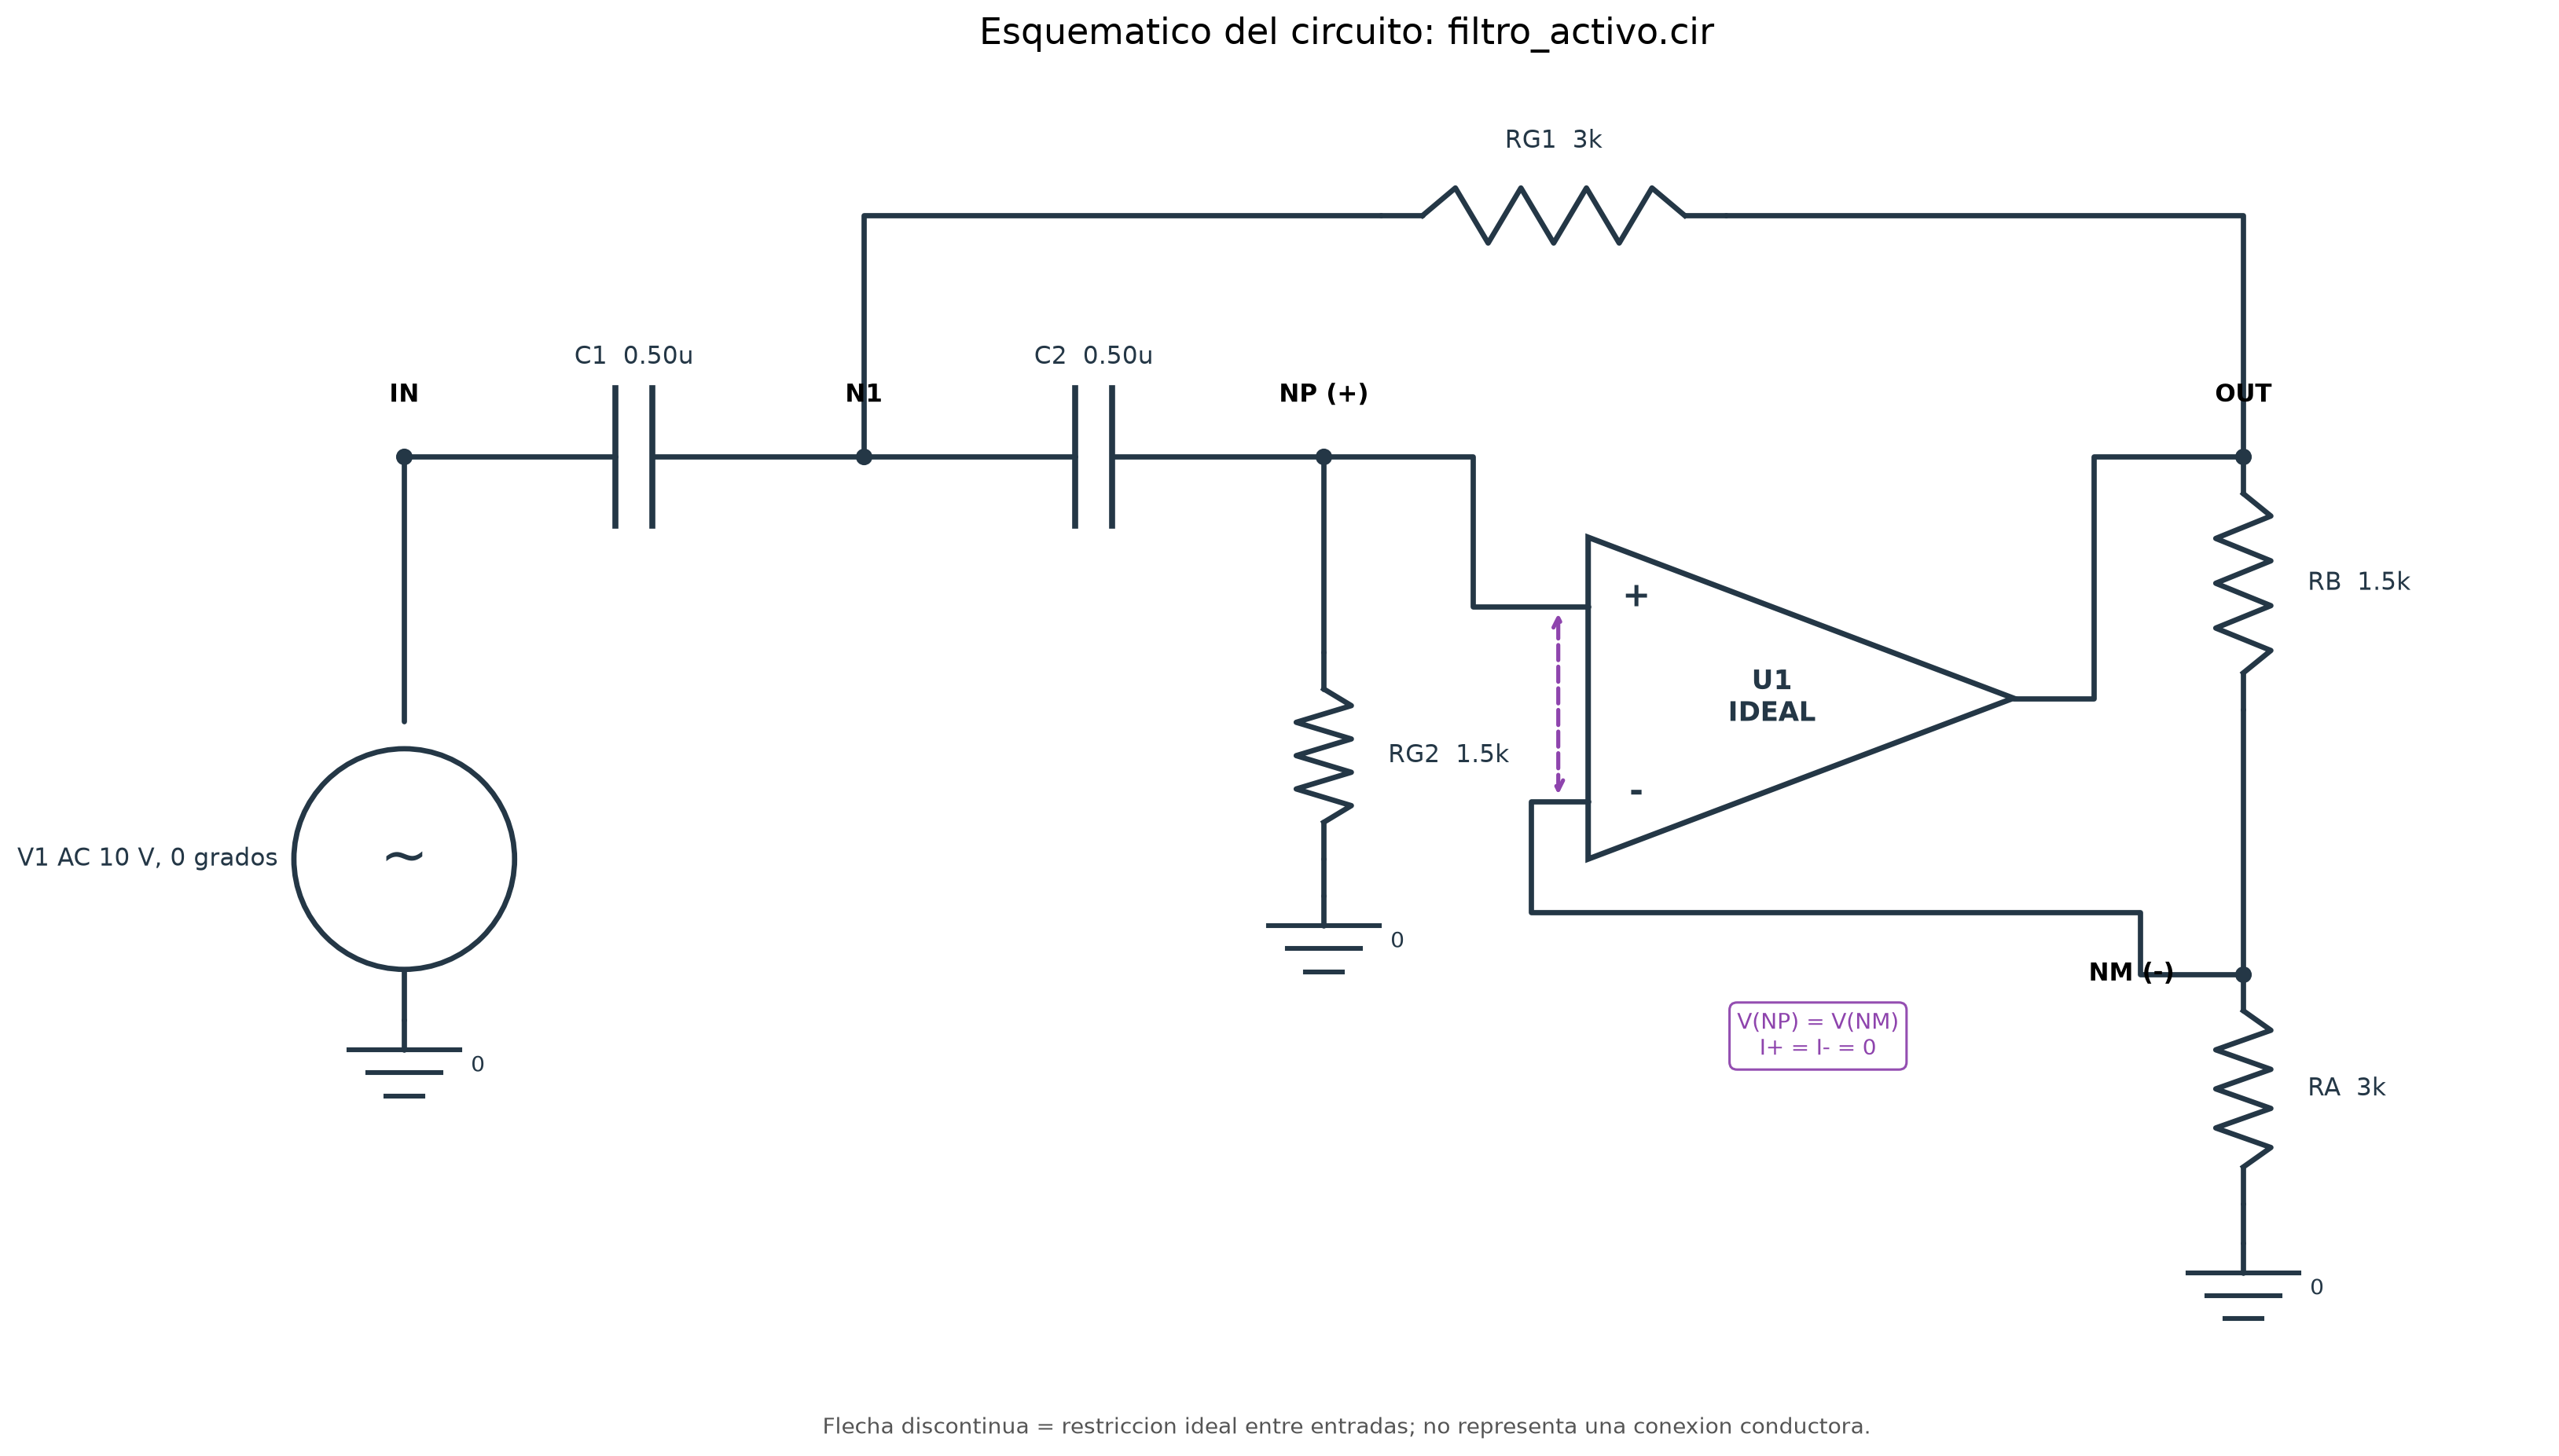
\includegraphics[width=0.78\linewidth]{2_circuito_objetivo_modificado_agent/plots/esquematico_filtro_activo.png}
\caption{Esquemático del filtro activo modificado.}
\end{figure}

\subsection{Topología y formulación}
La validación del netlist fue \textbf{Satisfactorio}. El análisis AC mediante MNA también fue \textbf{Satisfactorio}: 300 de 300 puntos fueron validados. La gráfica de topología conserva las conexiones del circuito; el op-amp ideal se representa mediante la restricción del modelo, no como una rama pasiva.

\begin{figure}[H]
\centering
\includegraphics[width=0.78\linewidth]{2_circuito_objetivo_modificado_agent/plots/graph.png}
\caption{Grafo orientado del circuito modificado.}
\end{figure}

La matriz Tableau mostrada a continuación es \textbf{parcial}: se construye sin el bloque $U1$ y no resuelve el circuito completo. La solución válida del op-amp se obtiene con MNA; la matriz MNA completa a 10 Hz se incluye después.

\begin{figure}[H]
\centering
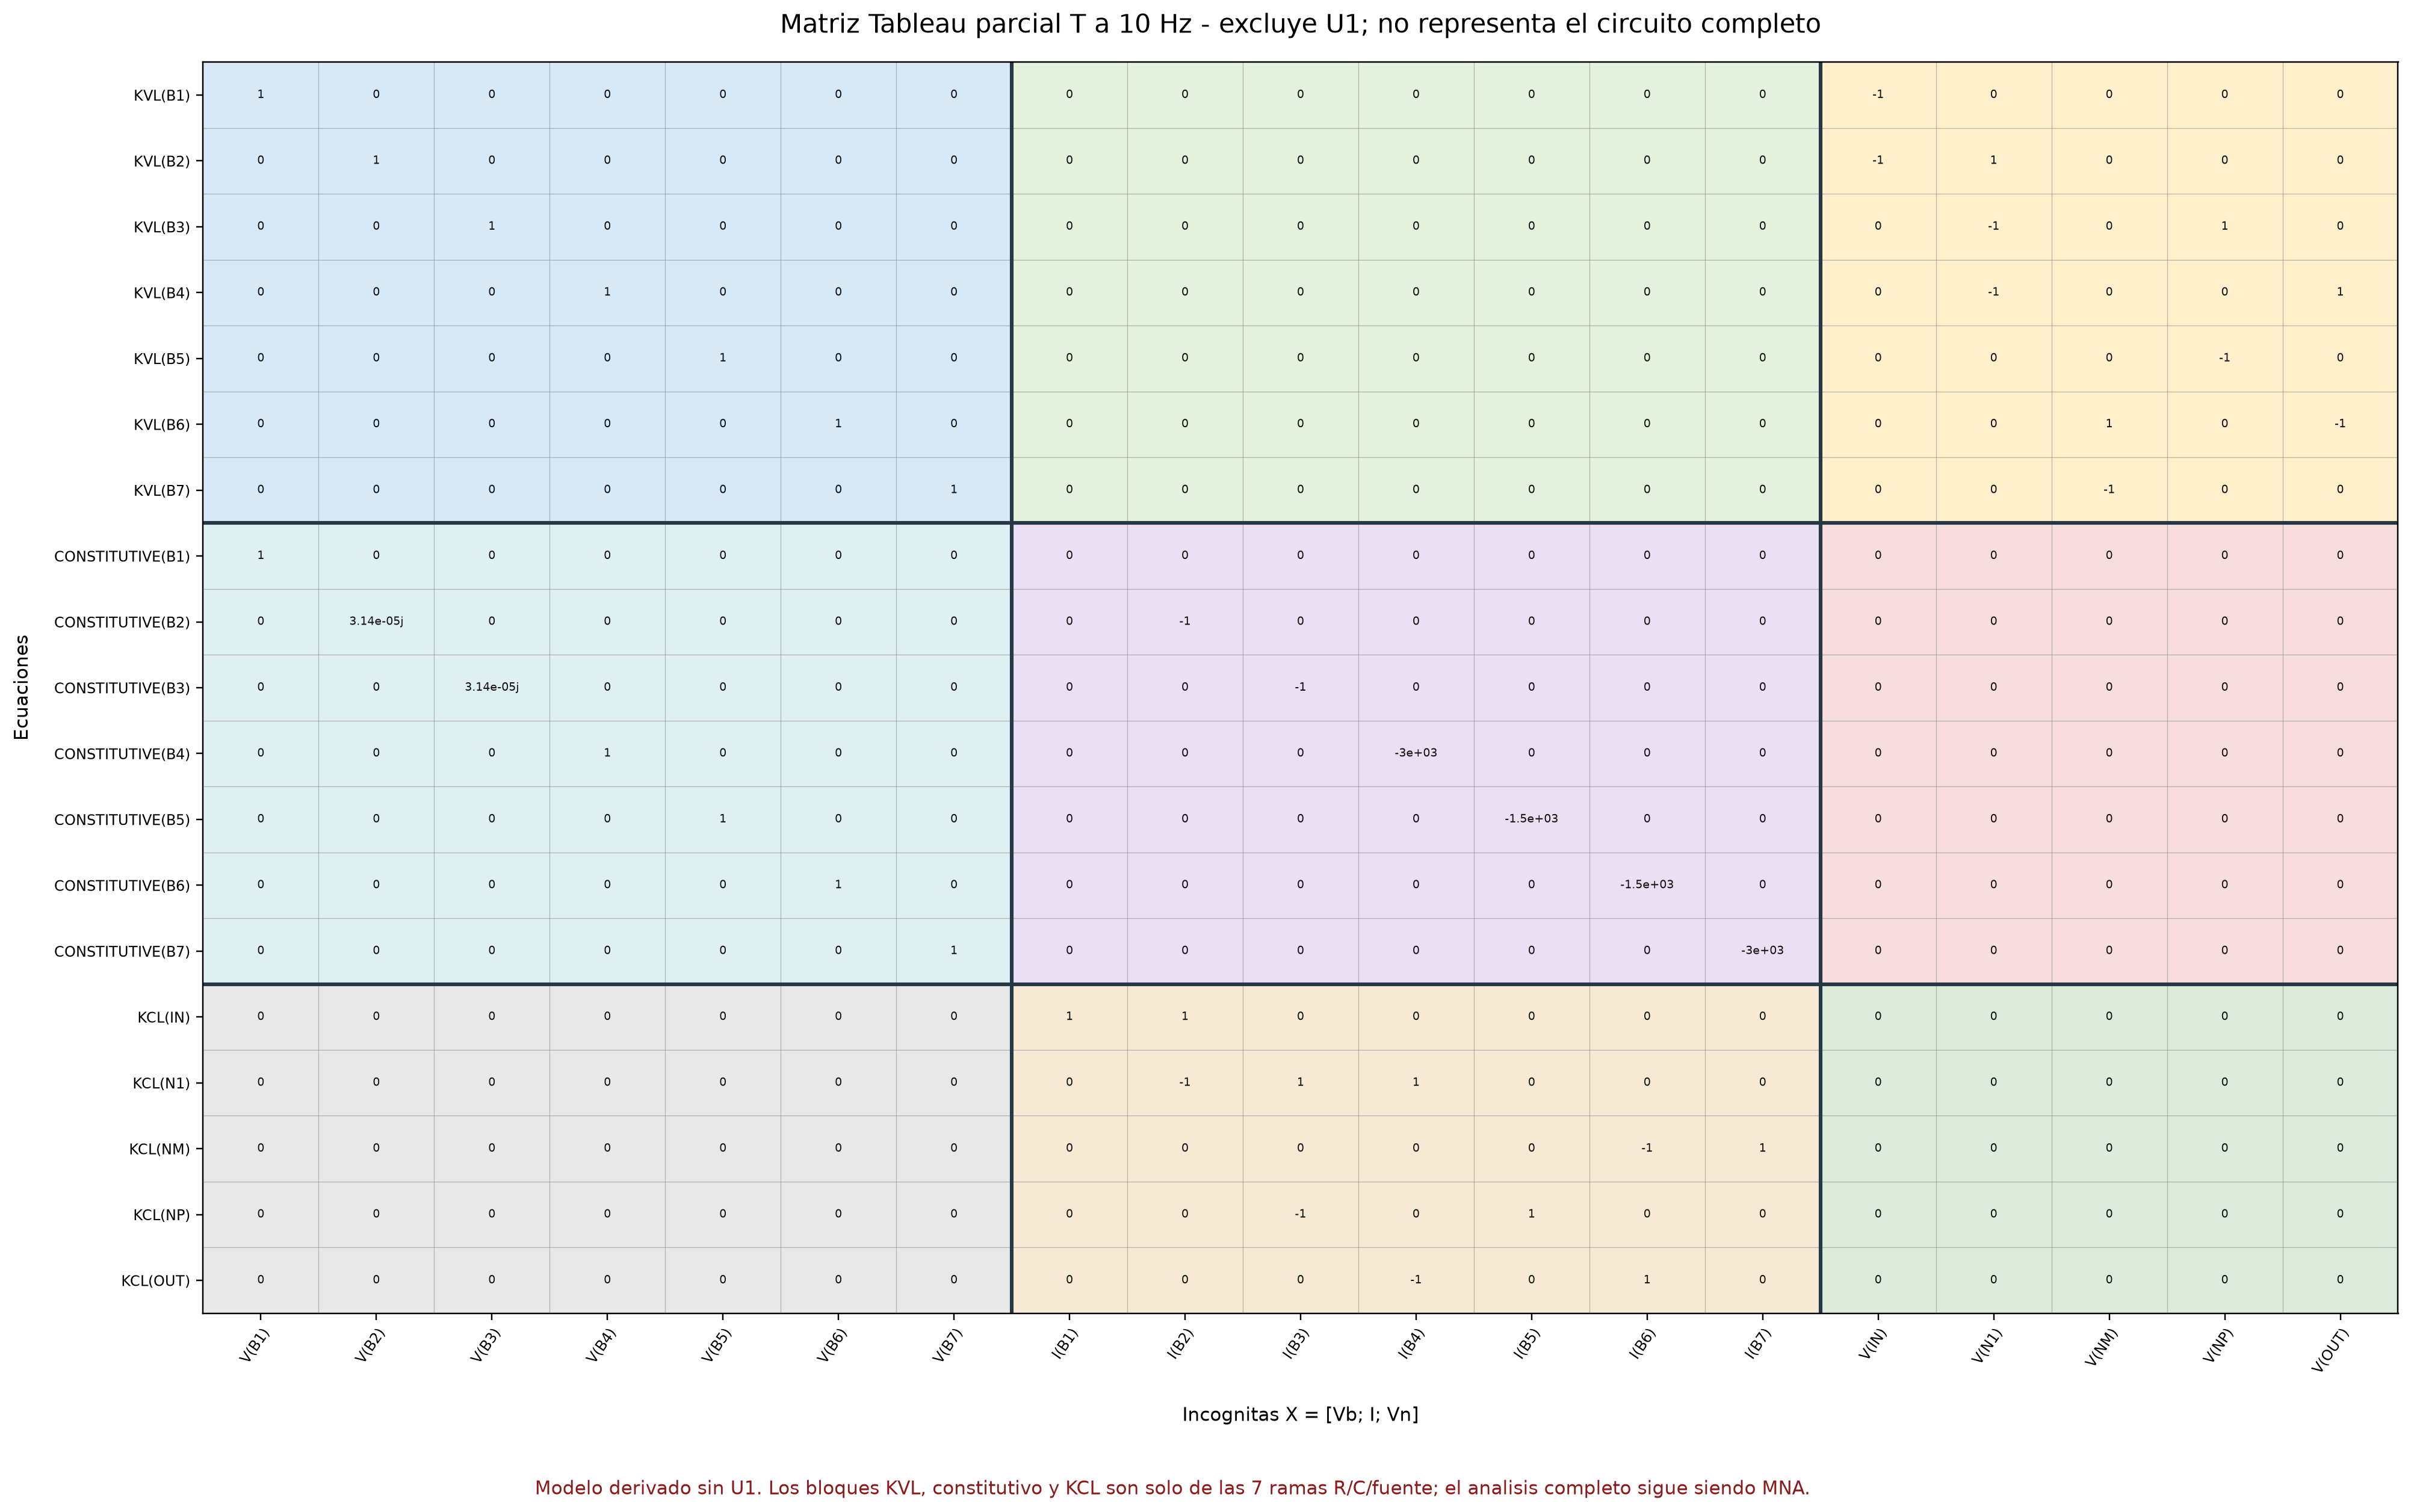
\includegraphics[width=0.9\linewidth]{2_circuito_objetivo_modificado_agent/plots/tableau_partial_T_colored_blocks_10Hz.png}
\caption{Matriz Tableau parcial a 10 Hz; excluye el op-amp ideal.}
\end{figure}

\begin{figure}[H]
\centering
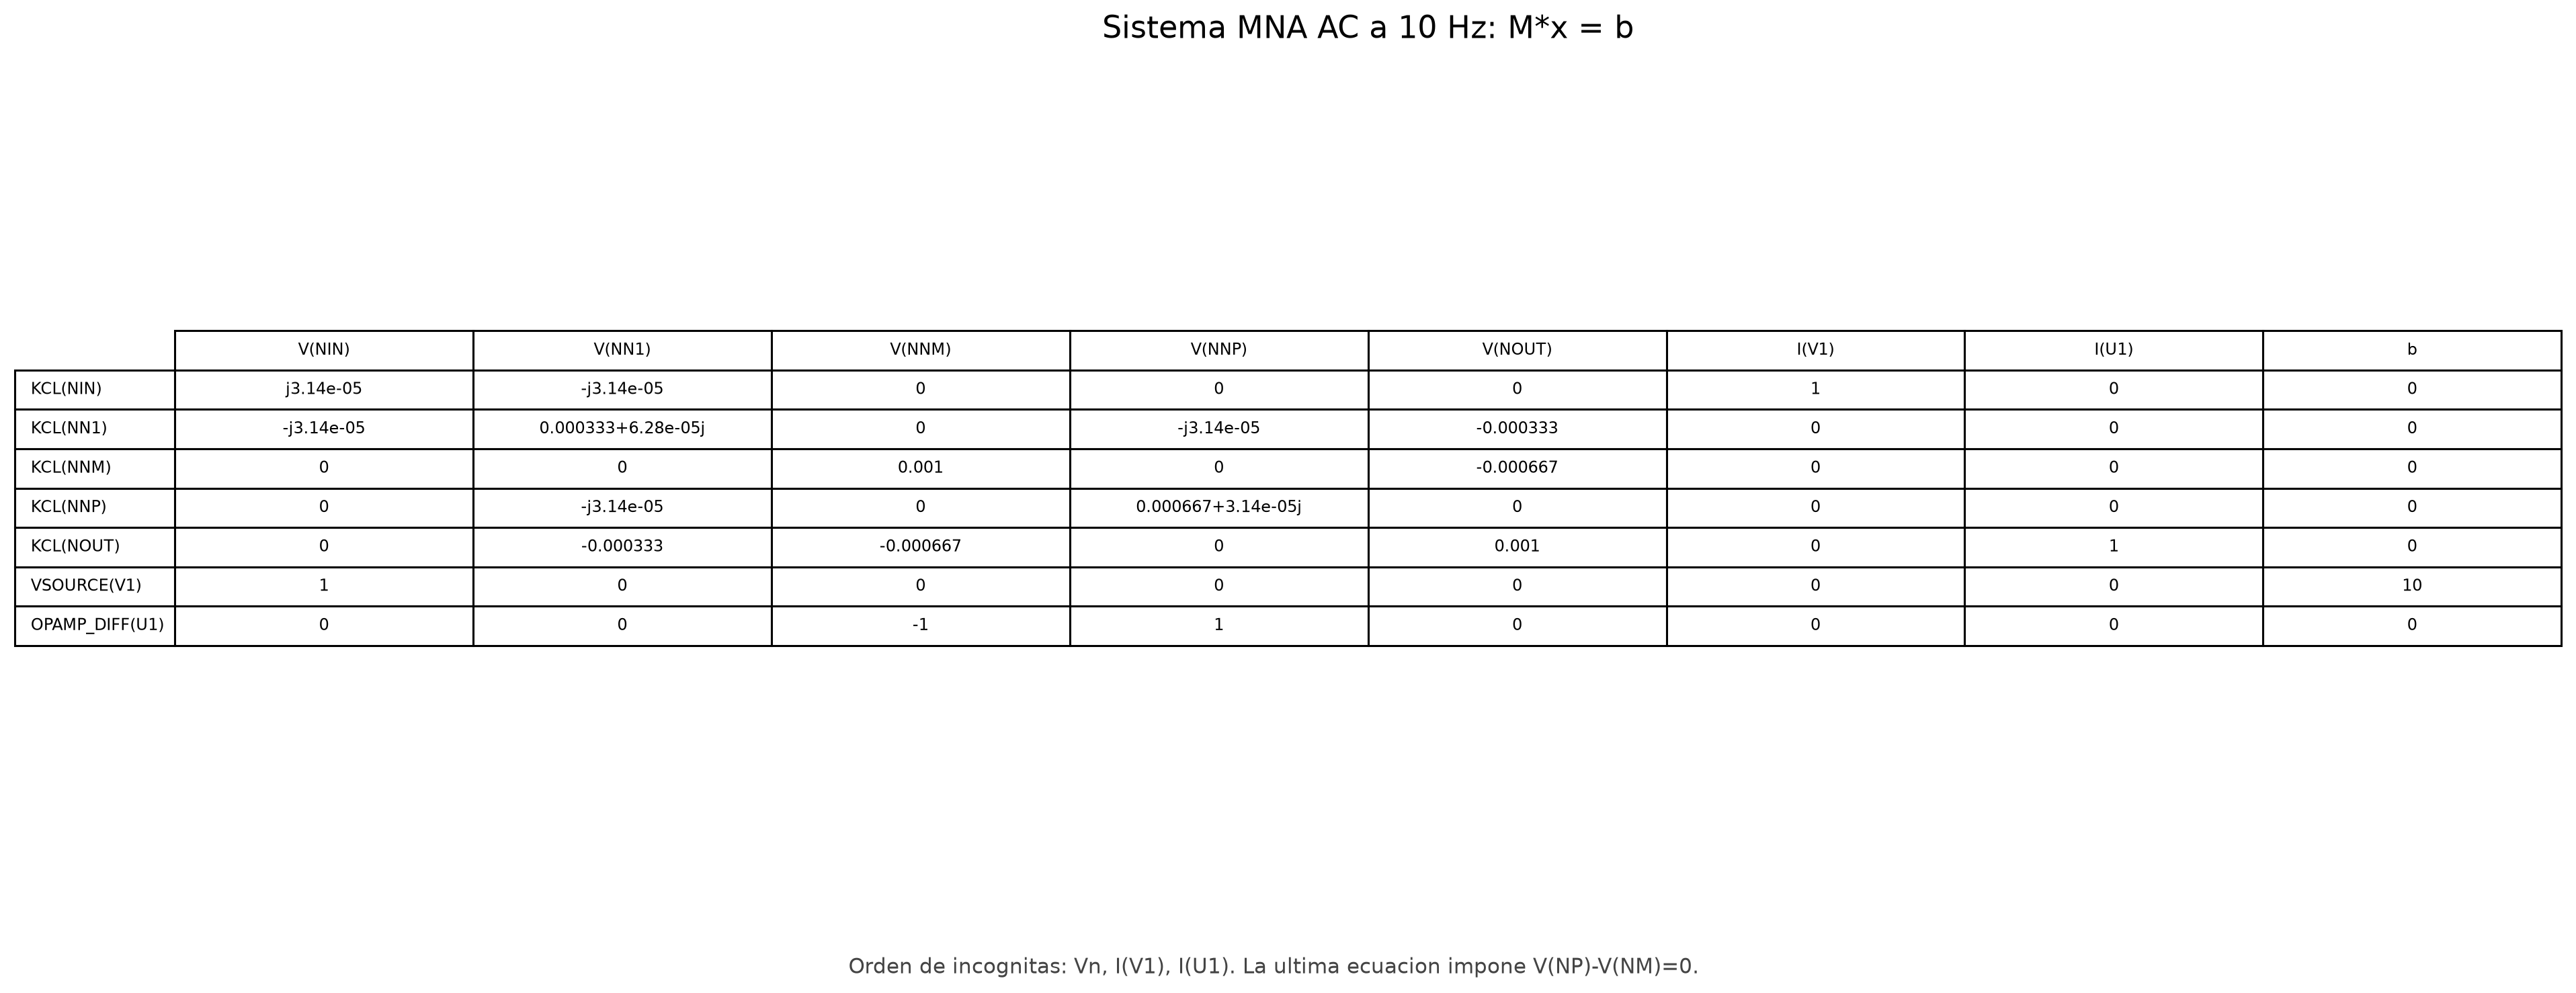
\includegraphics[width=0.95\linewidth]{../../filtro_activo_20261116_1710_circuito_objetivo_modificado/mna_system_10Hz.png}
\caption{Sistema MNA AC completo del circuito a 10 Hz.}
\end{figure}

\subsection{Resultados del analisis en AC del Agente y HSPICE}
Para documentar la transferencia se ejecutó el barrido MNA de 300 puntos sobre los artefactos normalizados de esta ejecución, solicitando explícitamente $H(w)=V(OUT)/V(IN)$. El barrido adicional reportó estado global \textbf{Satisfactorio}. Los valores de la tabla proceden del agente SPICE.

\begin{table}[H]
\centering
\begin{tabular}{lrrr}
\toprule
Punto & Frecuencia (Hz) & $H(w)$ (dB) & Fase ($^\circ$) \\
\midrule
Inicio & 10 & -43.6069 & 170.5933 \\
Fin & 100000 & 3.5218 & 0.2128 \\
\bottomrule
\end{tabular}
\caption{Valores representativos de la transferencia del circuito modificado.}
\end{table}

La magnitud de voltaje de salida informada directamente por el agente SPICE fue 0.0660172 V a 10 Hz y 14.99993 V a 100 kHz. Las figuras presentan la magnitud de transferencia, el voltaje de salida y la fase.

\begin{figure}[H]
\centering
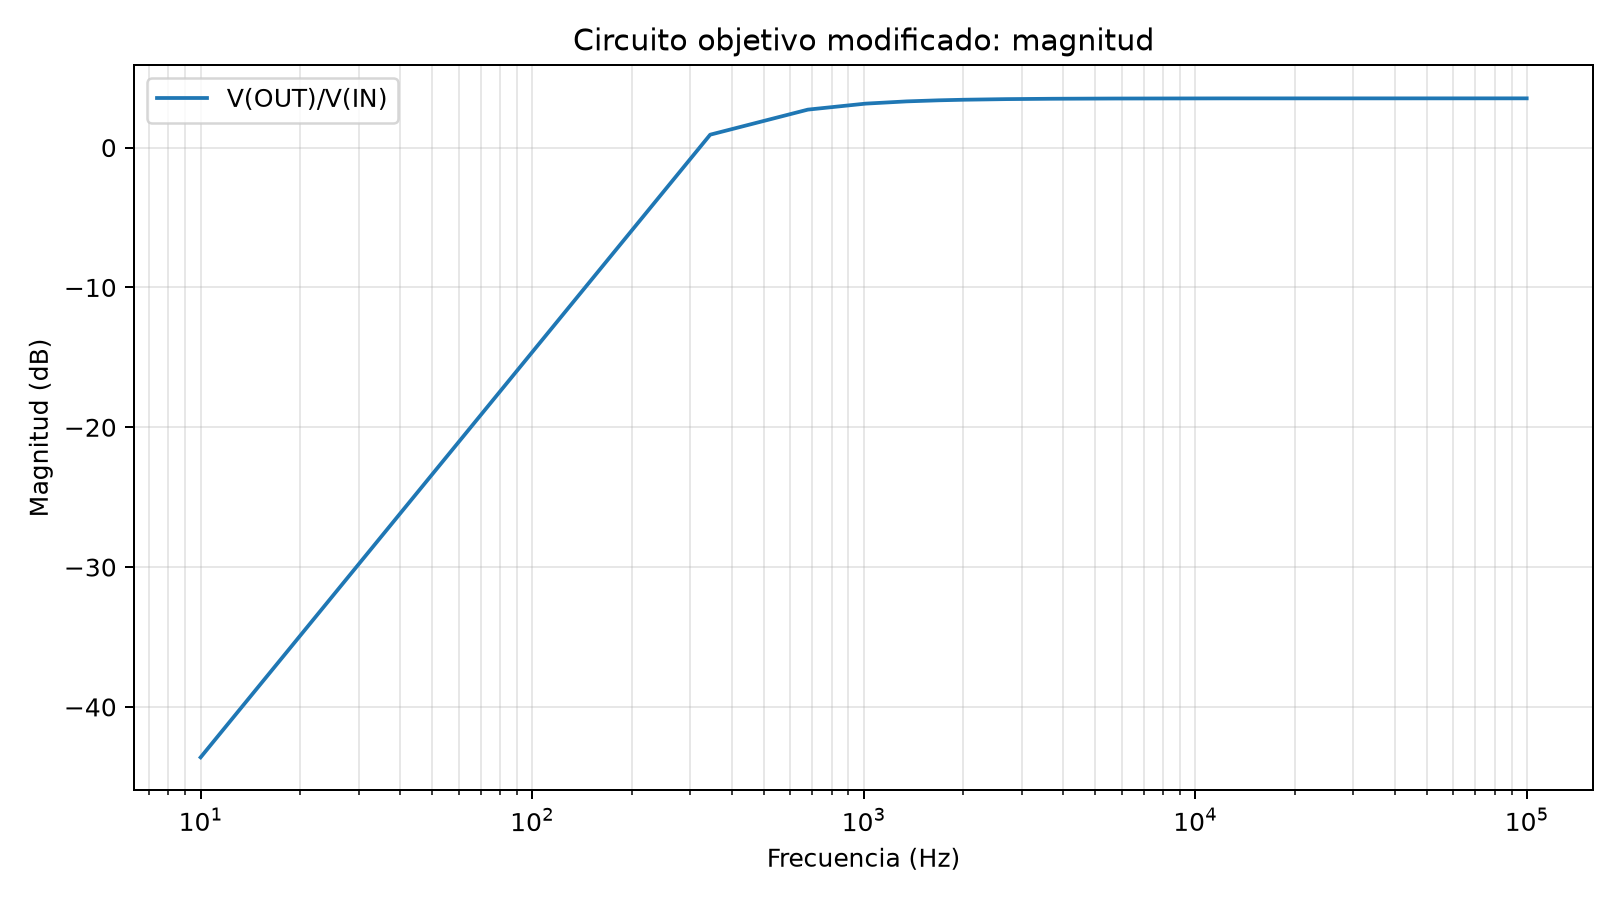
\includegraphics[width=0.78\linewidth]{../comparaciones_20261117_1306/caso2_plots/magnitude.png}
\caption{Gráfica de Magnitud en dB de la función de transferencia $H(w)$ obtenida por el agente.}
\end{figure}

\begin{figure}[H]
\centering
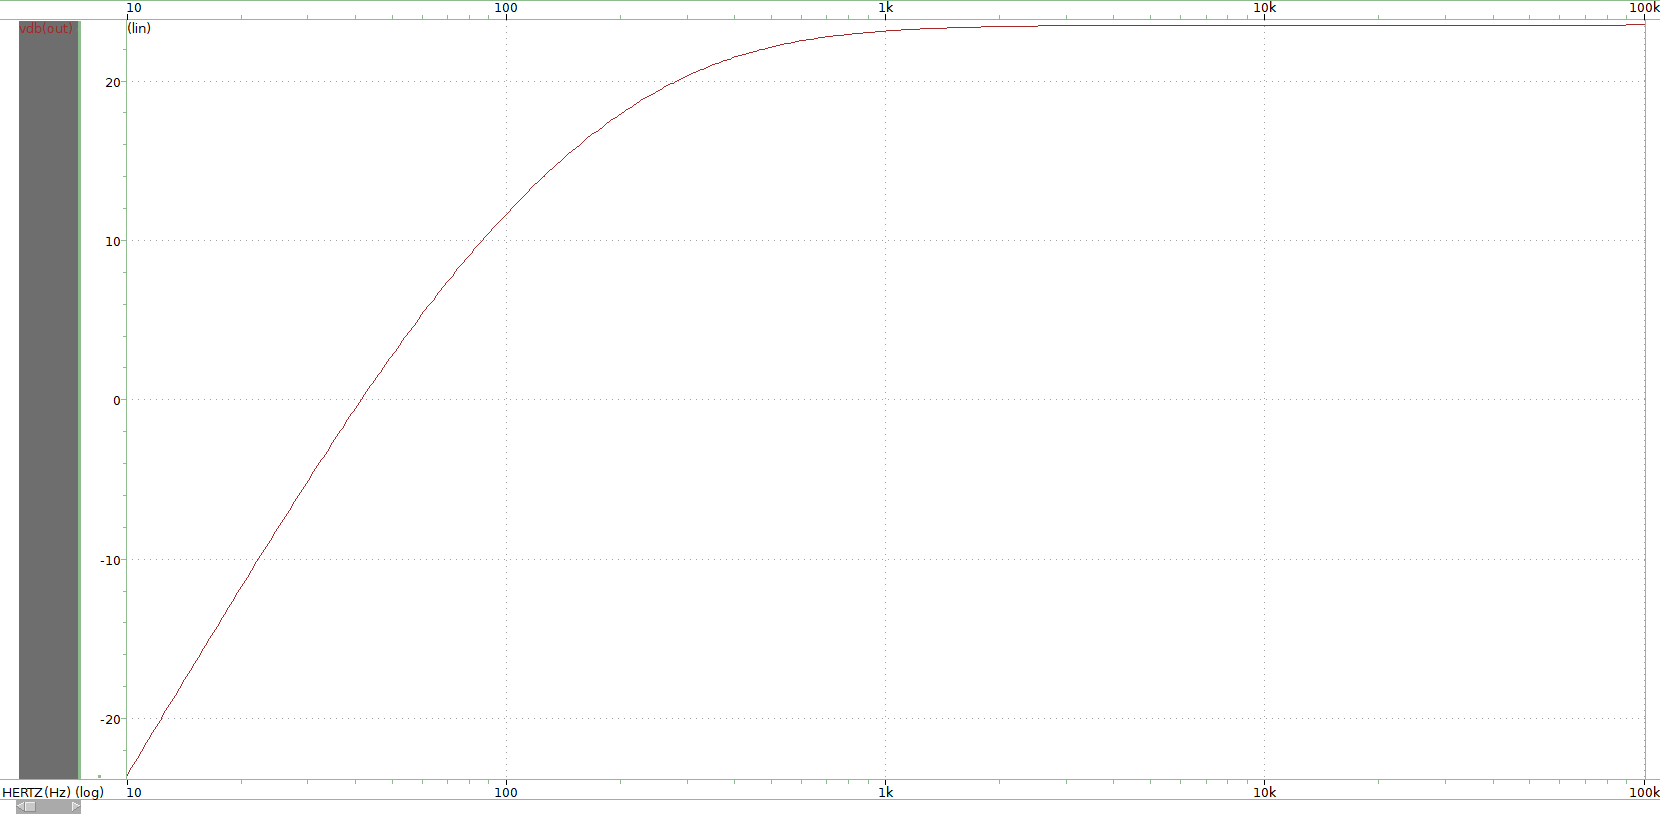
\includegraphics[width=0.78\linewidth]{2_circuito_objetivo_modificado_HSPICE/magnitude_dB.png}
\caption{Gráfica de Magnitud en dB de la función de transferencia $H(w)$ obtenida por HSPICE.}
\end{figure}

\begin{figure}[H]
\centering
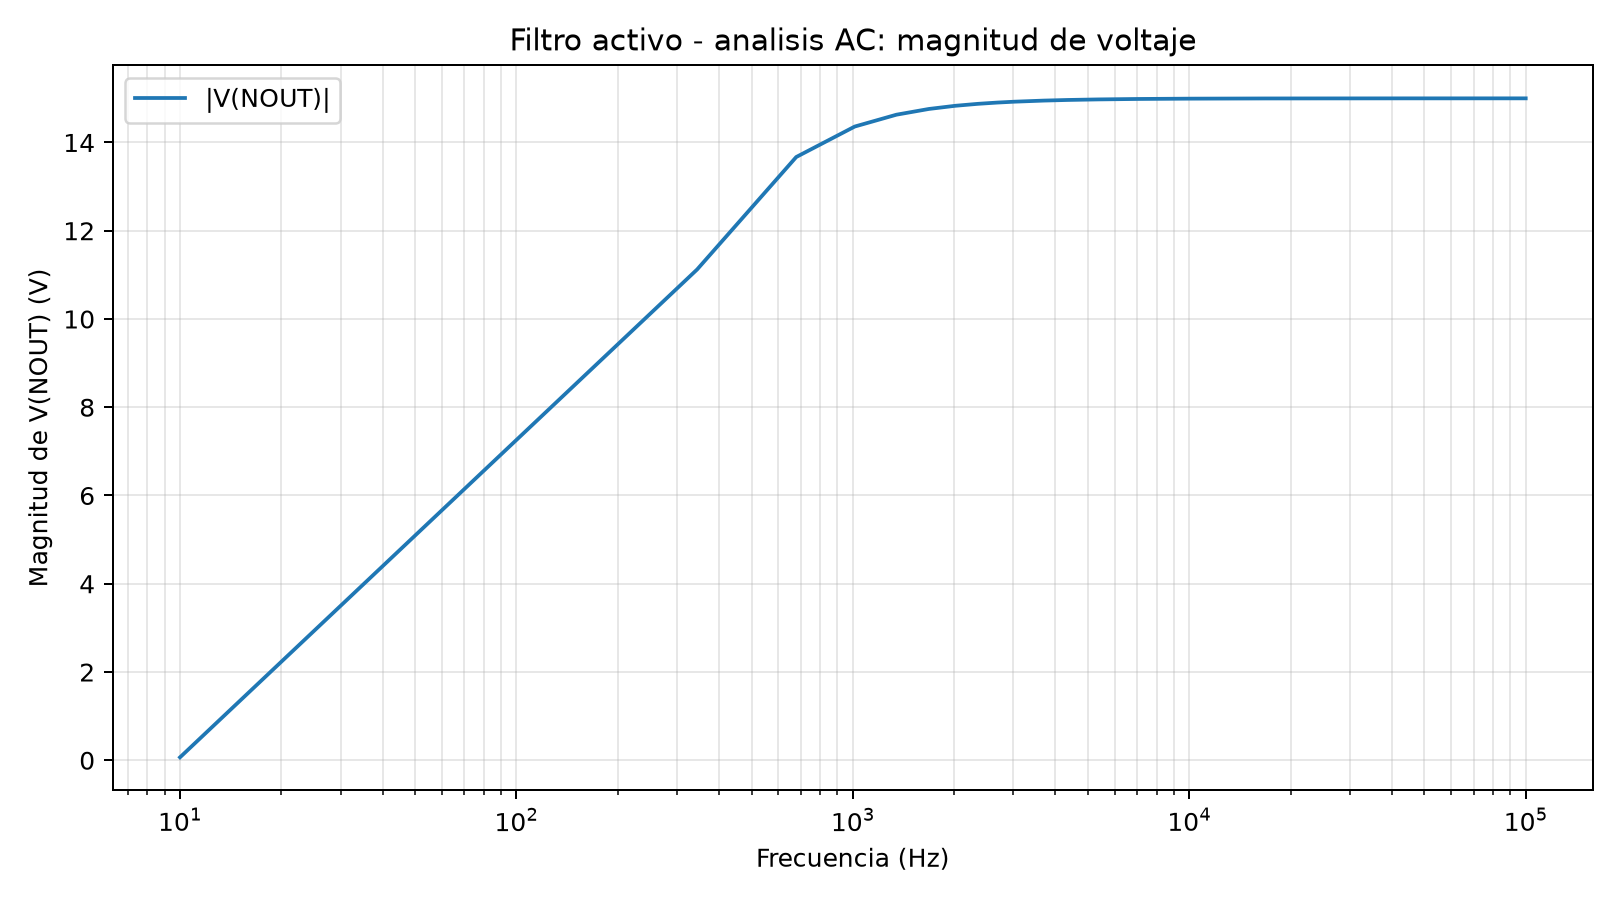
\includegraphics[width=0.78\linewidth]{2_circuito_objetivo_modificado_agent/plots/magnitude_voltage.png}
\caption{Gráfica de Magnitud en Voltaje de $V\_OUT$ obtenida por el agente.}
\end{figure}

\begin{figure}[H]
\centering
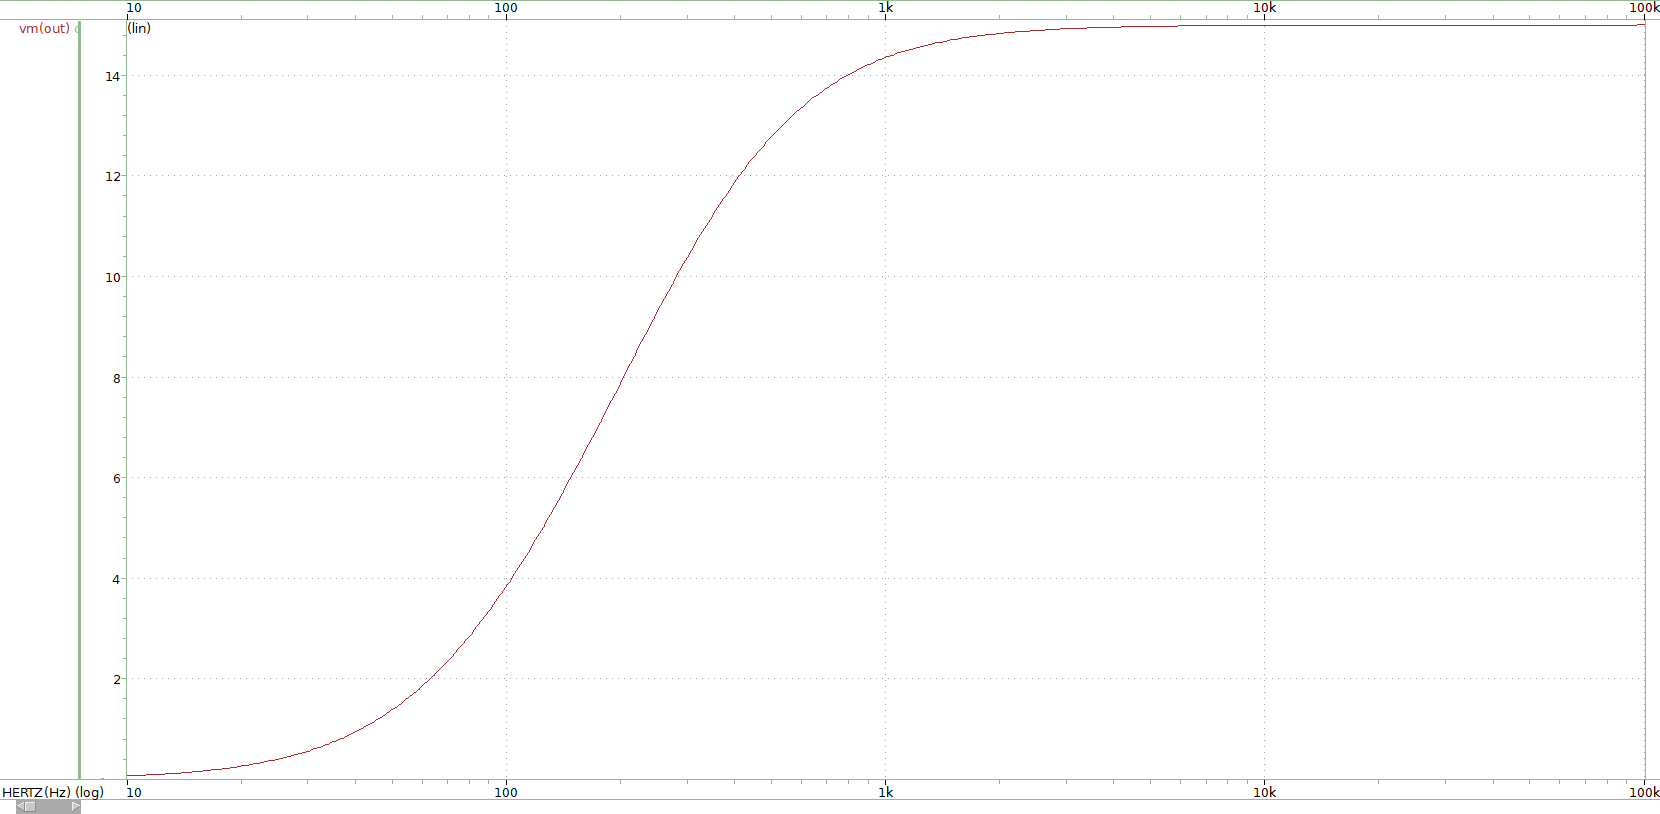
\includegraphics[width=0.78\linewidth]{2_circuito_objetivo_modificado_HSPICE/magnitude_voltage.png}
\caption{Gráfica de Magnitud en Voltaje de $V\_OUT$ obtenida por HSPICE.}
\end{figure}

\begin{figure}[H]
\centering
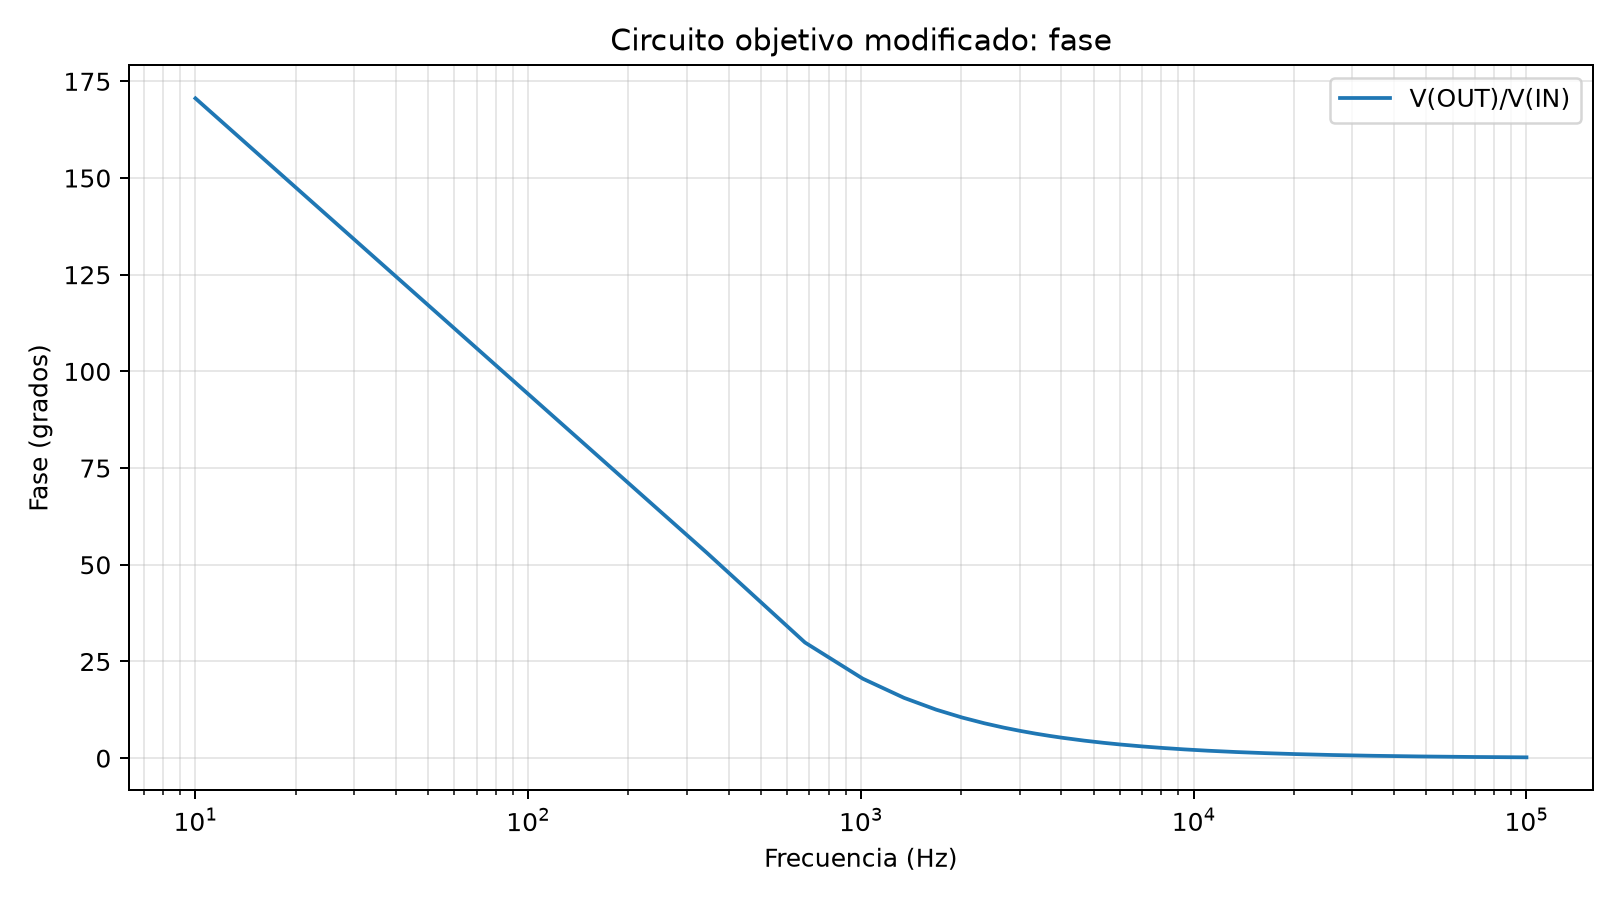
\includegraphics[width=0.78\linewidth]{../comparaciones_20261117_1306/caso2_plots/phase.png}
\caption{Gráfica de Fase de la función de transferencia $H(w)$ obtenida por el agente.}
\end{figure}


\begin{figure}[H]
\centering
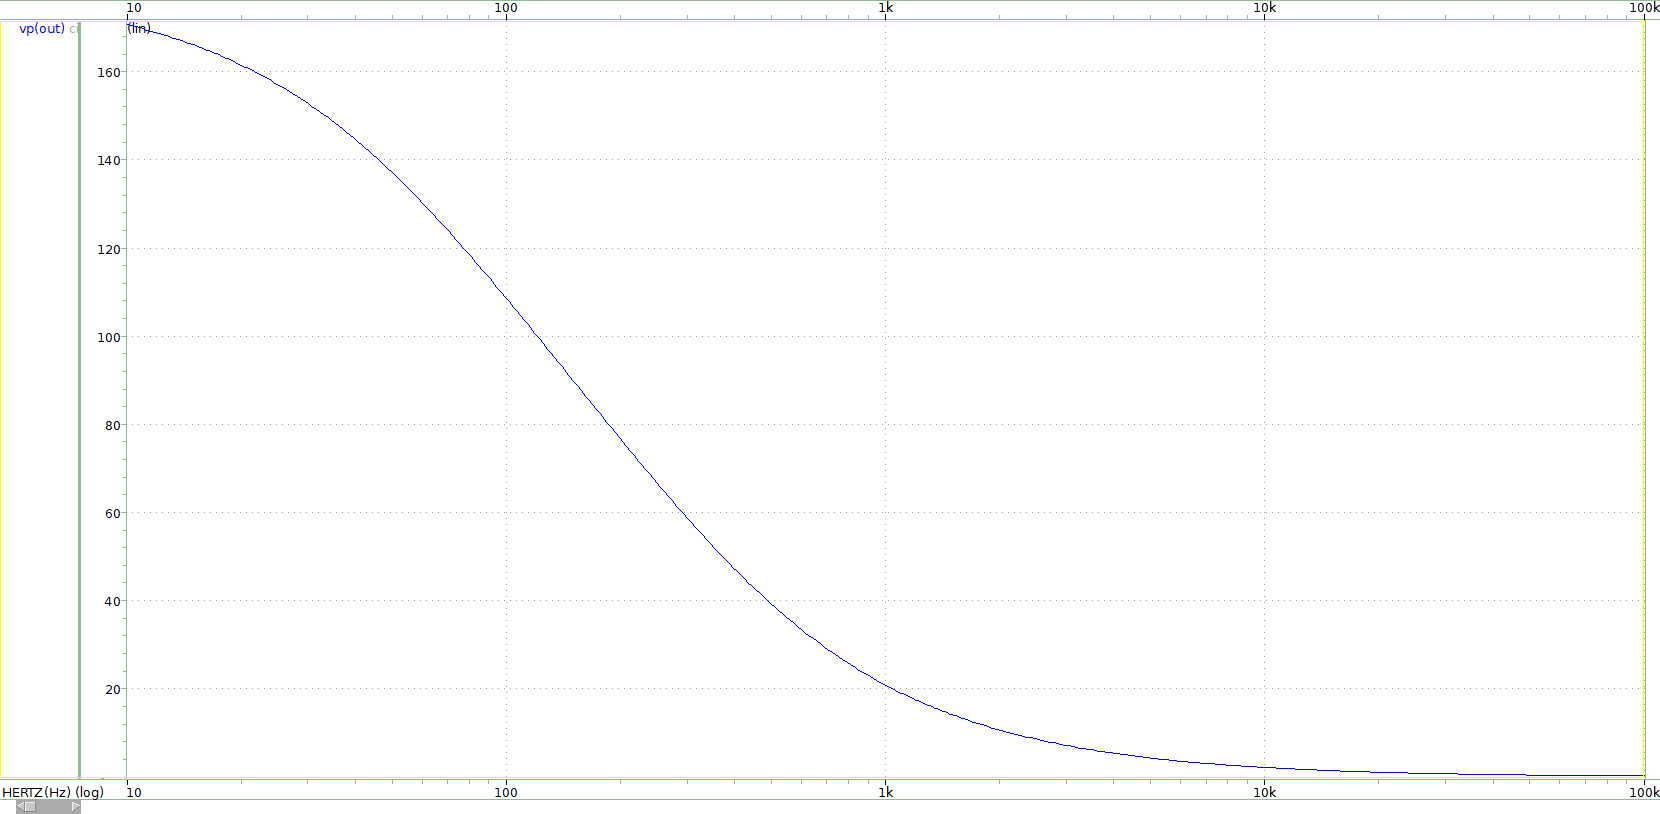
\includegraphics[width=0.78\linewidth]{2_circuito_objetivo_modificado_HSPICE/phase.png}
\caption{Gráfica de Fase de la función de transferencia $H(w)$ obtenida por HSPICE.}
\end{figure}


\subsection{Comparación con HSPICE}
La referencia corresponde a los datos obtenidos por HSPICE. HSPICE usó 401 puntos DEC entre 10 Hz y 100 kHz, mientras que el agente usó 300 puntos LIN; por ello se compararon únicamente las dos frecuencias exactamente coincidentes, sin interpolación. Ambos circuitos usan una entrada AC de 10 V. La referencia aproxima el op-amp con una fuente dependiente de ganancia finita $10^9$, mientras que el agente emplea el modelo ideal MNA; por tanto, el acuerdo en los extremos no implica equivalencia de modelos ni valida todos los puntos del barrido.

La herramienta \texttt{compare\_reference.py} comparó los fasores de salida $V(NOUT)$ con tolerancias absoluta $10^{-6}$ V y relativa $2\times10^{-5}$. Los fasores, errores y estados siguientes proceden de su artefacto de comparación.

\begin{table}[H]
\centering
\small
\begin{tabularx}{\linewidth}{lXX}
\toprule
Frecuencia & Agente MNA: $V(NOUT)$ (V) & HSPICE: $V(OUT)$ (V) \\
\midrule
10 Hz & $-6.51294636\times10^{-2}+j1.07899595\times10^{-2}$ & $-6.51294704\times10^{-2}+j1.07899388\times10^{-2}$ \\
100 kHz & $14.99982691+j5.57037127\times10^{-2}$ & $14.99979657+j5.57036035\times10^{-2}$ \\
\bottomrule
\end{tabularx}
\caption{Fasores de salida en los puntos de frecuencia coincidentes.}
\end{table}

\begin{table}[H]
\centering
\begin{tabular}{lrrc}
\toprule
Frecuencia & Error absoluto (V) & Error relativo & Estado \\
\midrule
10 Hz & $2.1769\times10^{-8}$ & $3.2974\times10^{-7}$ & \textbf{PASS} \\
100 kHz & $3.0342\times10^{-5}$ & $2.0228\times10^{-6}$ & \textbf{PASS} \\
\bottomrule
\end{tabular}
\caption{Comparación compleja de voltajes de salida; resultado global \textbf{Satisfactorio} (2/2 puntos).}
\end{table}

La gráfica HSPICE $VDB(OUT)$ está en dBV (voltaje de salida), mientras que la gráfica del agente está en dB de $V(OUT)/V(IN)$; por la entrada de 10 V, estas magnitudes no tienen la misma referencia y no deben compararse directamente. La comparación cuantitativa se realiza con los fasores de salida en voltios y cubre únicamente los dos puntos coincidentes.


La comparación es reproducible con los artefactos JSON de puntos, referencia HSPICE y resultado de \texttt{compare\_reference.py}, conservados en la carpeta de comparación del reporte. %(Caso 2)
	\section{Circuito RLC diferente (Caso 3)}

\subsection{Parámetros y método}
El circuito analizado es una red RLC serie excitada por una fuente AC de 1 V. La salida se mide en $OUT$, sobre la resistencia $R_1$. Aunque el netlist denomina al circuito ``pasa-altas'', la salida sobre la resistencia presenta una respuesta resonante de banda: disminuye tanto en el extremo bajo como en el alto del barrido.

\begin{table}[H]
\centering
\begin{tabular}{ll}
\toprule
Parámetro & Valor \\
\midrule
Frecuencia de inicio y final & 10 Hz y 100 kHz \\
Tipo de barrido & Lineal, 400 puntos \\
Fuente $V_1$ & 1 V AC, $0^\circ$ \\
$C_1$ & 1 $\mu$F \\
$L_1$ & 10 mH \\
$R_1$ & 1 k$\Omega$ \\
Salida & $V(OUT)$ sobre $R_1$ \\
Formulación & Tableau completa \\
\bottomrule
\end{tabular}
\caption{Parámetros del circuito RLC diferente.}
\end{table}

\begin{figure}[H]
\centering
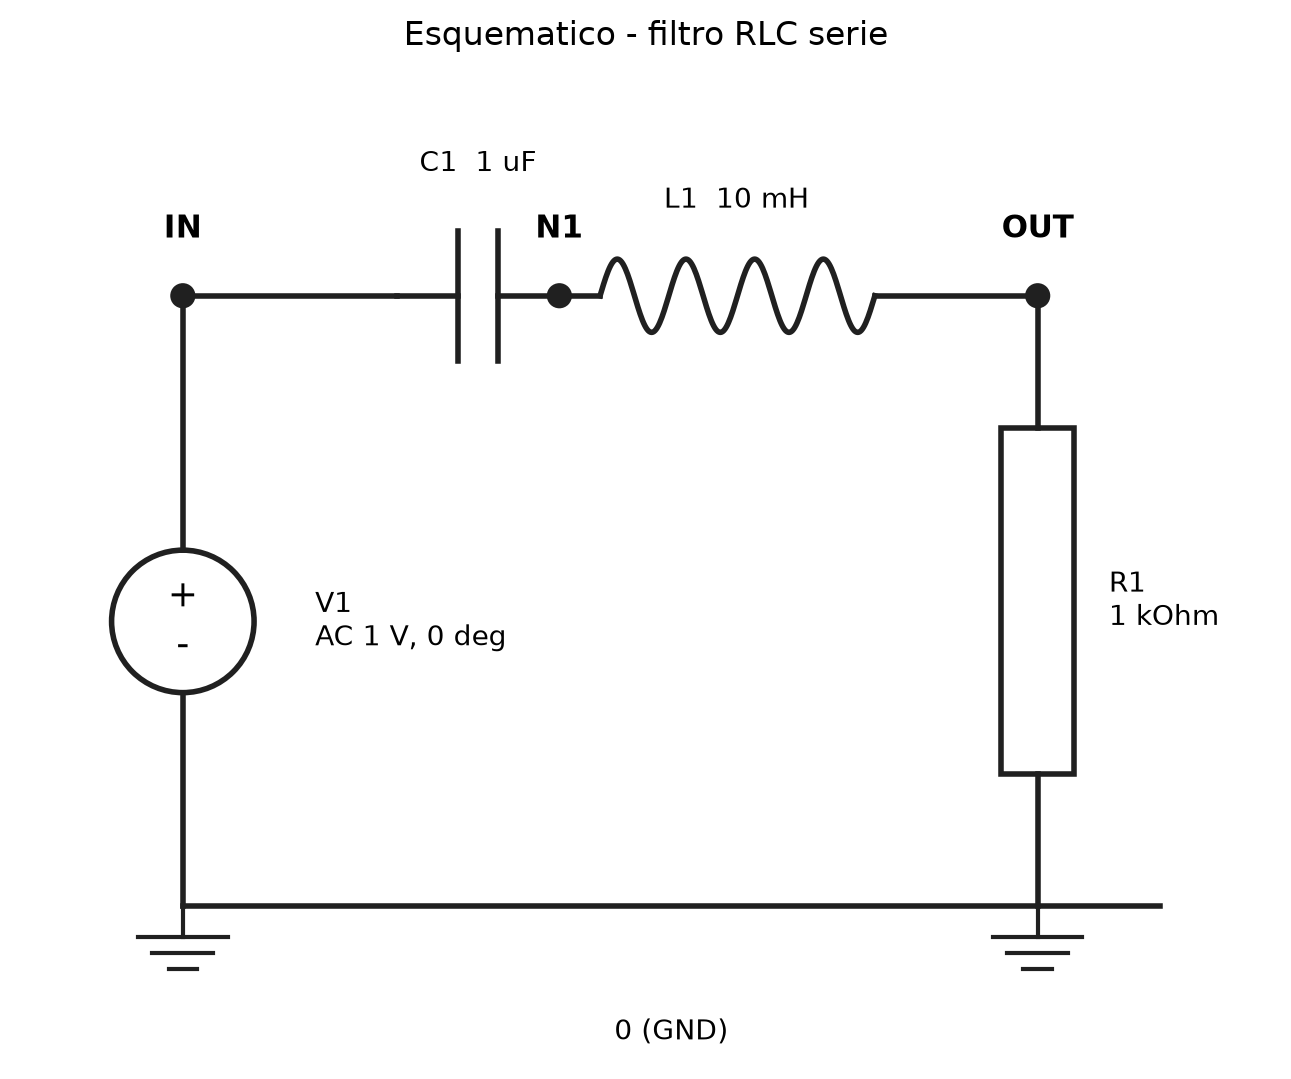
\includegraphics[width=0.78\linewidth]{3_circuito_dif_agent/plots/esquematico_filtro_pasa_altas.png}
\caption{Esquemático del circuito RLC serie.}
\end{figure}

\subsection{Topología, Tableau y validación}
La validación del netlist fue \textbf{Satisfactorio}. El circuito se ensambló mediante Tableau completo, de dimensión $11\times11$. La validación del sistema Tableau a 10 Hz fue \textbf{Satisfactorio} en sus cinco comprobaciones; el número de condición reportado fue $3.4574\times10^6$. En el barrido AC, el estado global fue \textbf{Satisfactorio} y los 400 puntos se validaron.

\begin{figure}[H]
\centering
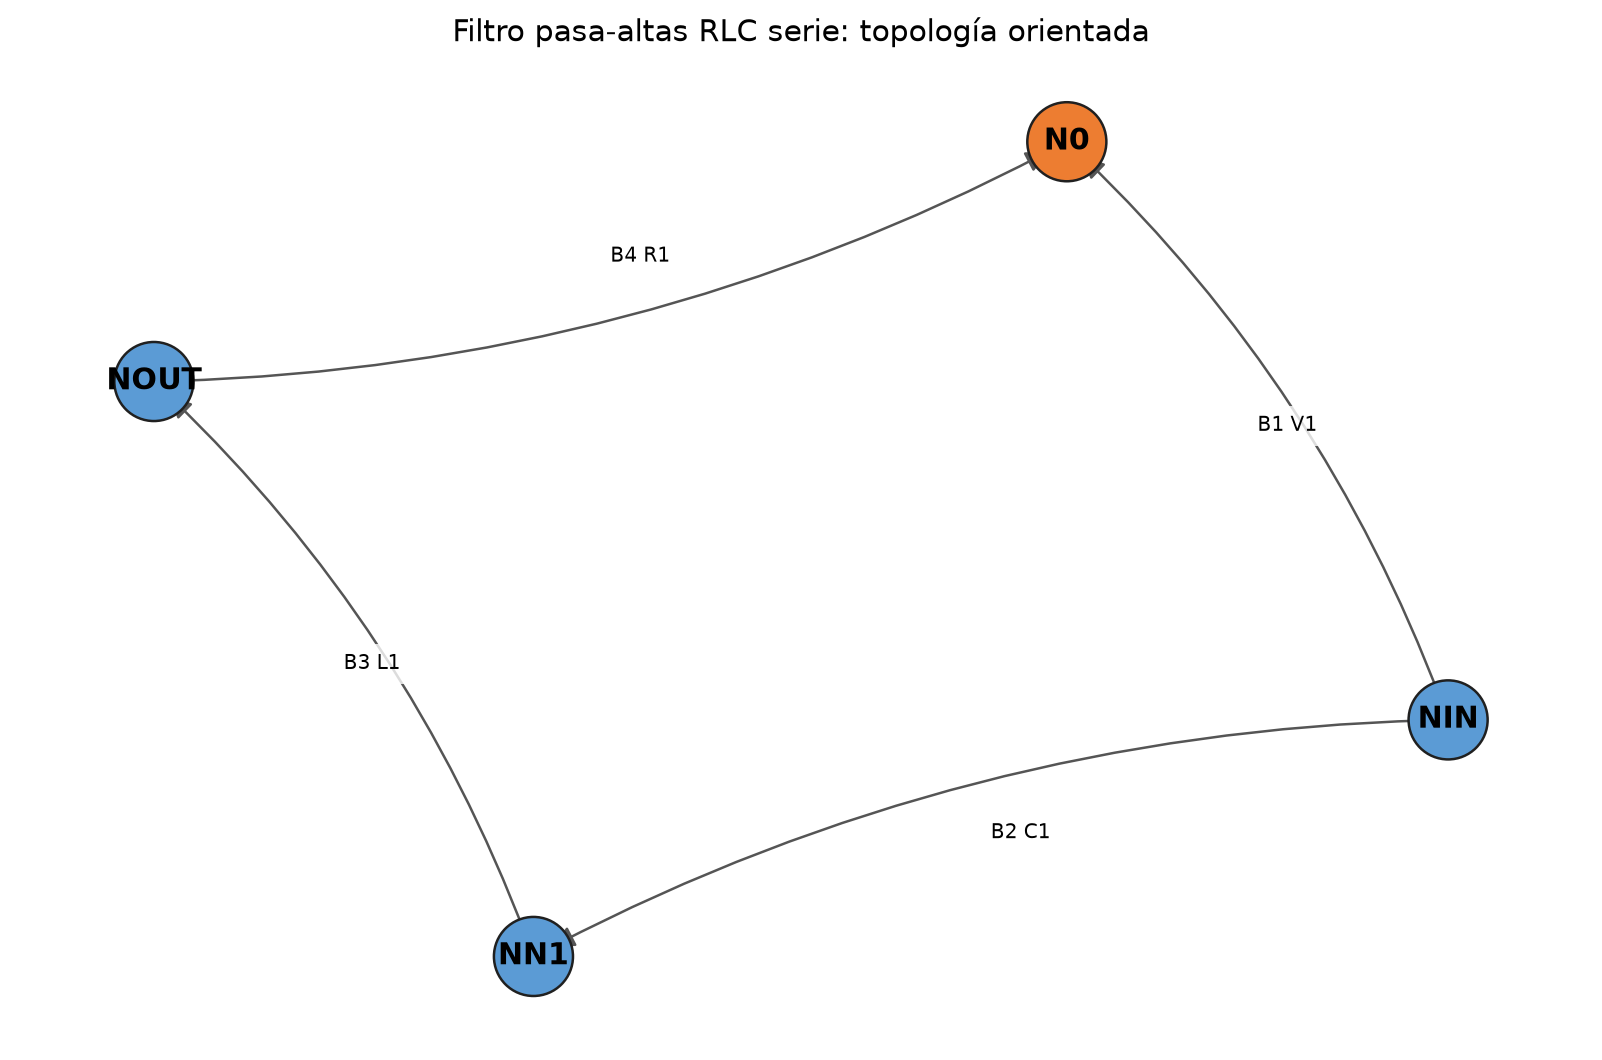
\includegraphics[width=0.78\linewidth]{3_circuito_dif_agent/plots/graph.png}
\caption{Grafo orientado de la red RLC.}
\end{figure}

\begin{figure}[H]
\centering
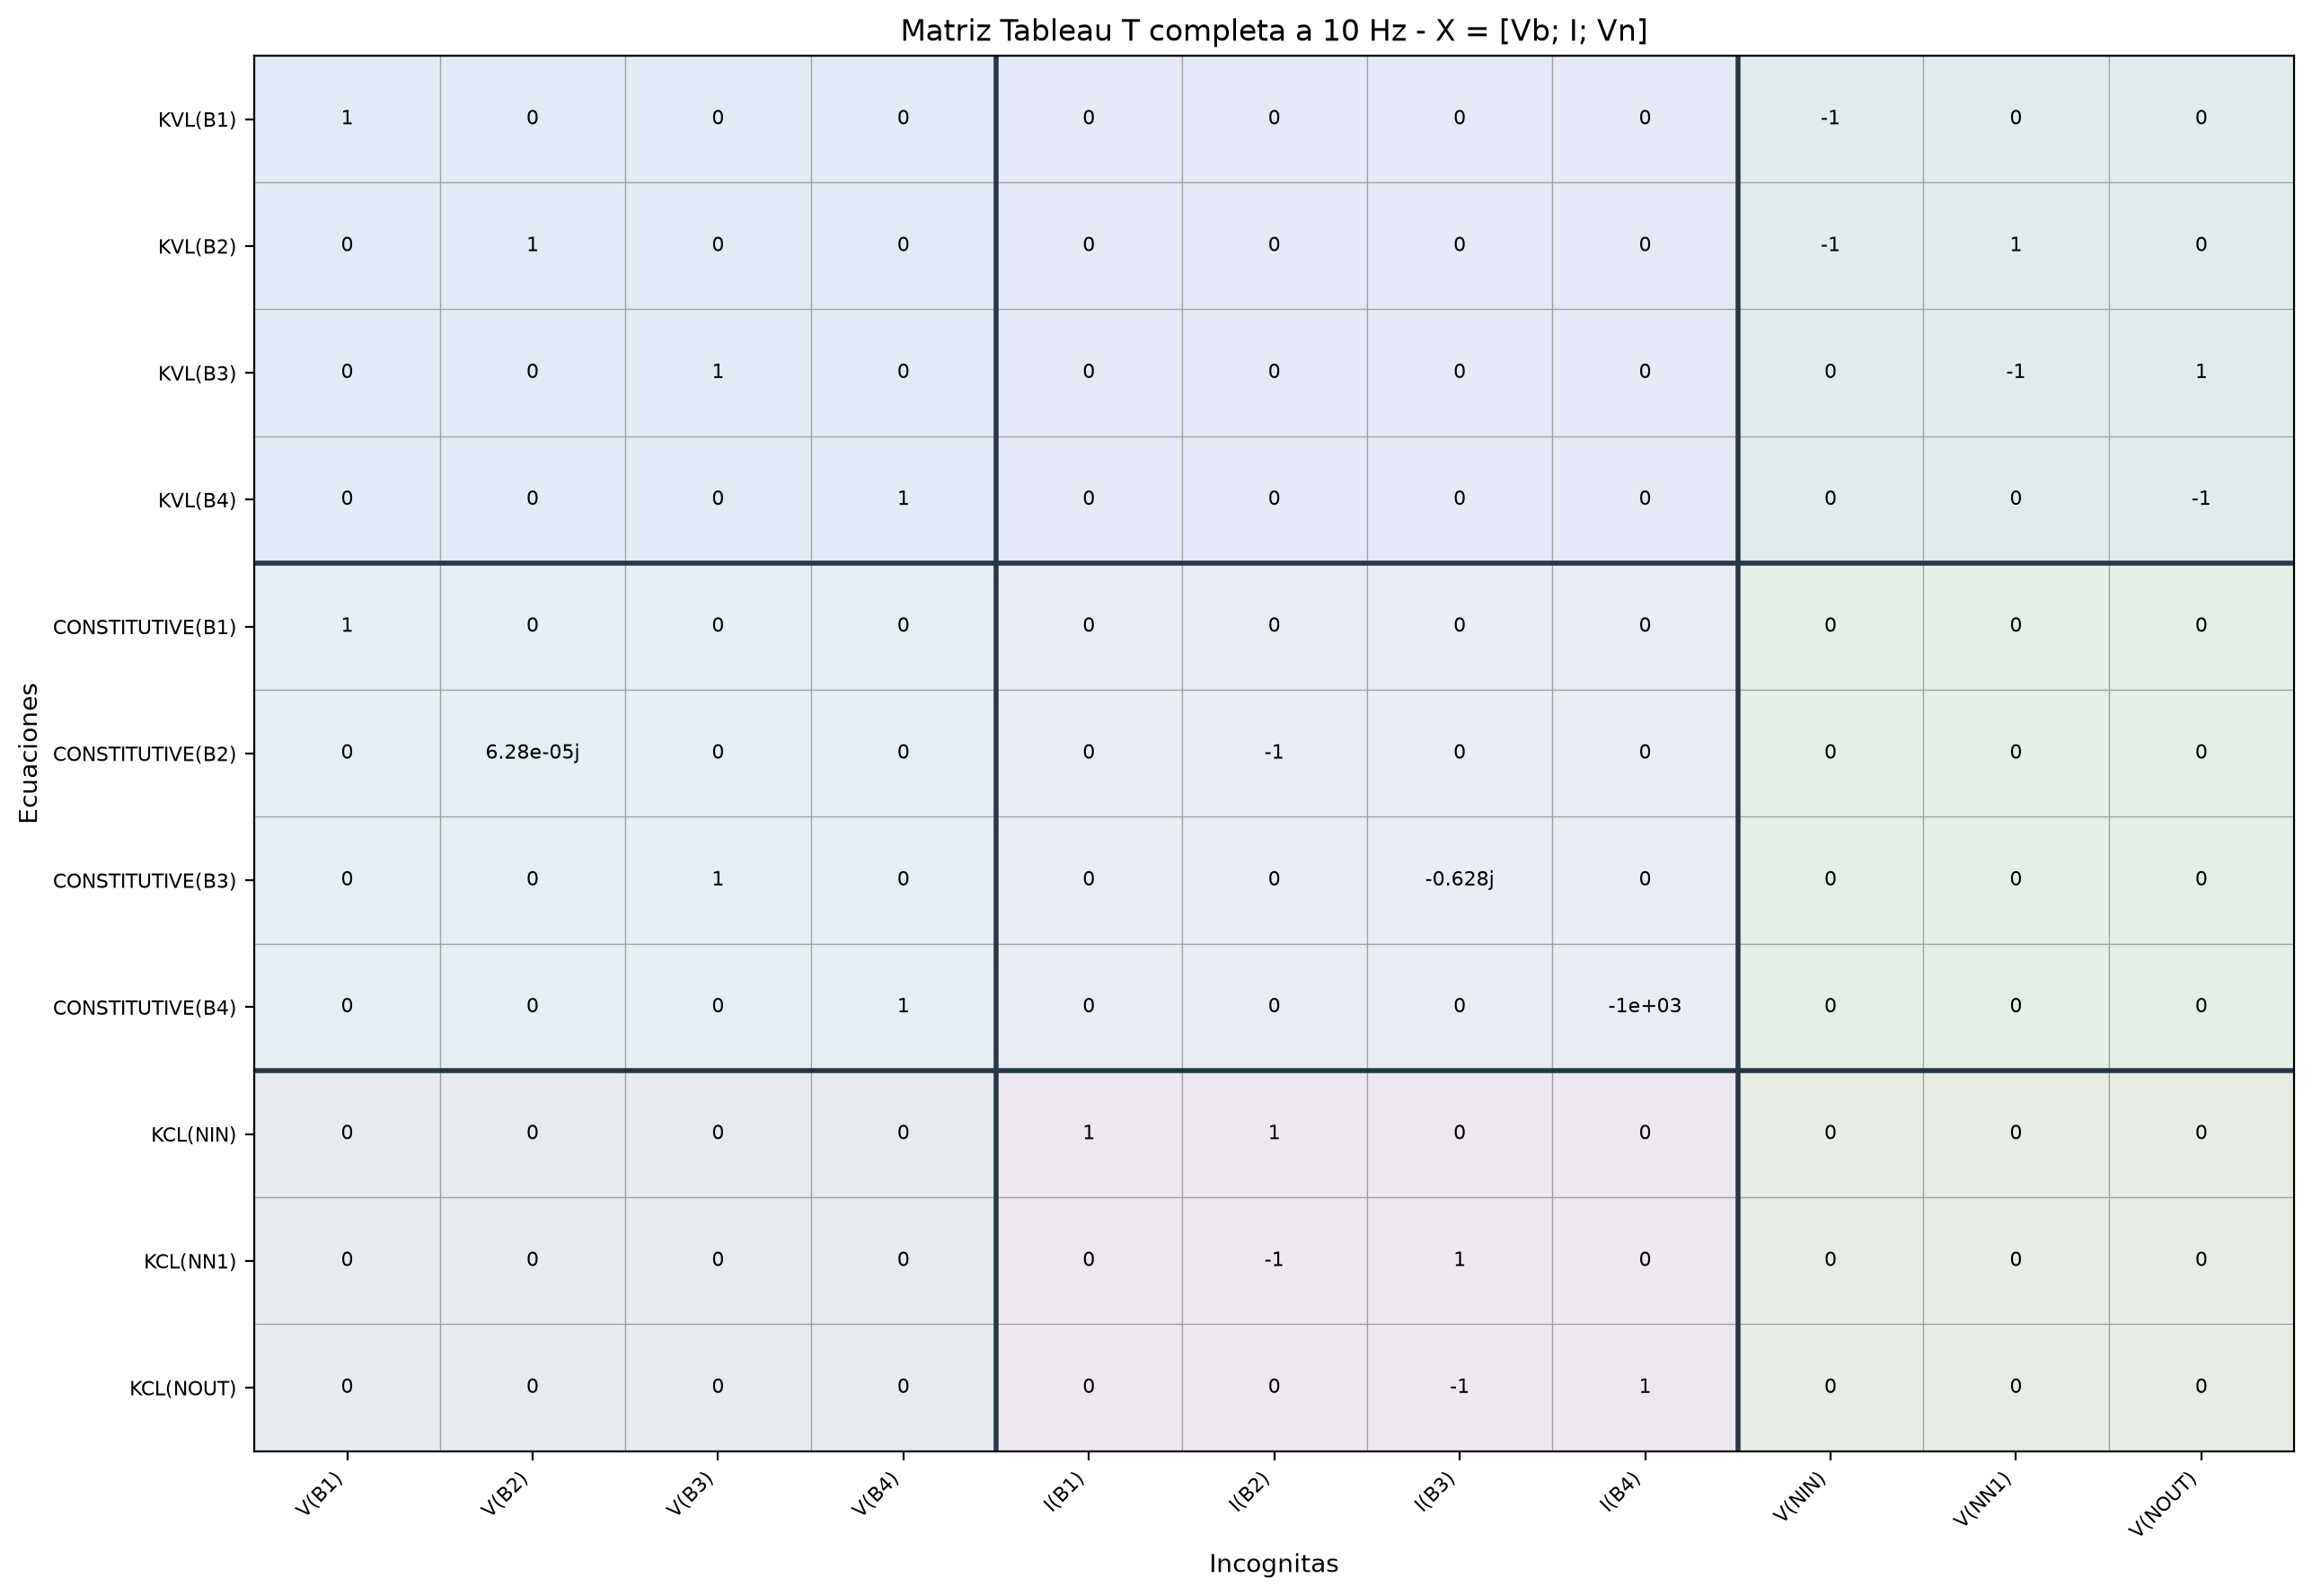
\includegraphics[width=0.95\linewidth]{3_circuito_dif_agent/plots/tableau_T_10Hz.png}
\caption{Matriz Tableau completa $T$ a 10 Hz, con $X=[V_b; I; V_n]$.}
\end{figure}

\subsection{Resultados del analisis en AC del Agente y HSPICE}
El observable es $V(OUT)/V(IN)$. Como la fuente AC tiene amplitud de 1 V, la magnitud de la transferencia coincide numéricamente con la magnitud del voltaje de salida en voltios. Los valores siguientes proceden del Agente y corresponden al inicio, al máximo muestreado del barrido y al final.

\begin{table}[H]
\centering
\begin{tabular}{lrrr}
\toprule
Punto & Frecuencia (Hz) & Magnitud (dB) & Fase ($^\circ$) \\
\midrule
Inicio & 10 & -24.0532 & 86.4046 \\
Máximo muestreado & 1513.6090 & -0.0004383 & 0.5756 \\
Fin & 100000 & -16.0701 & -80.9547 \\
\bottomrule
\end{tabular}
\caption{Valores representativos de $V(OUT)/V(IN)$ obtenidos con Tableau.}
\end{table}

En esos mismos puntos, la magnitud de $V(OUT)$ reportada por el Agente fue 0.0627107 V, 0.9999495 V y 0.1572156 V, respectivamente.

\begin{figure}[H]
\centering
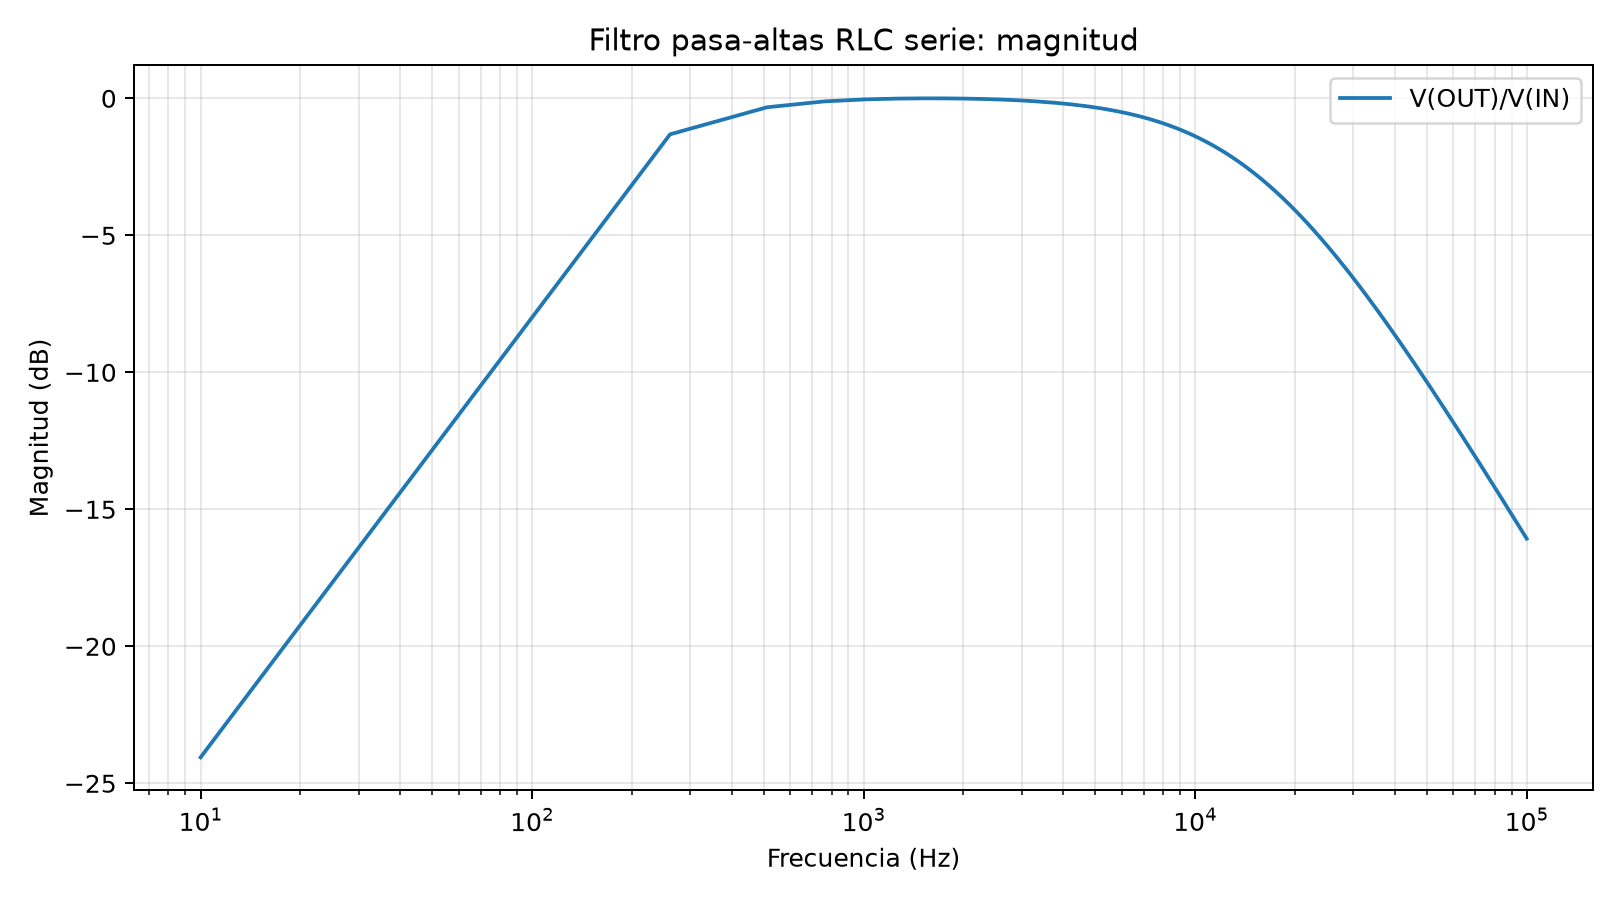
\includegraphics[width=0.70\linewidth]{3_circuito_dif_agent/plots/magnitude.png}
\caption{Gráfica de Magnitud en dB de la función de transferencia $H(w)$ obtenida por el agente.}
\end{figure}


\begin{figure}[H]
\centering
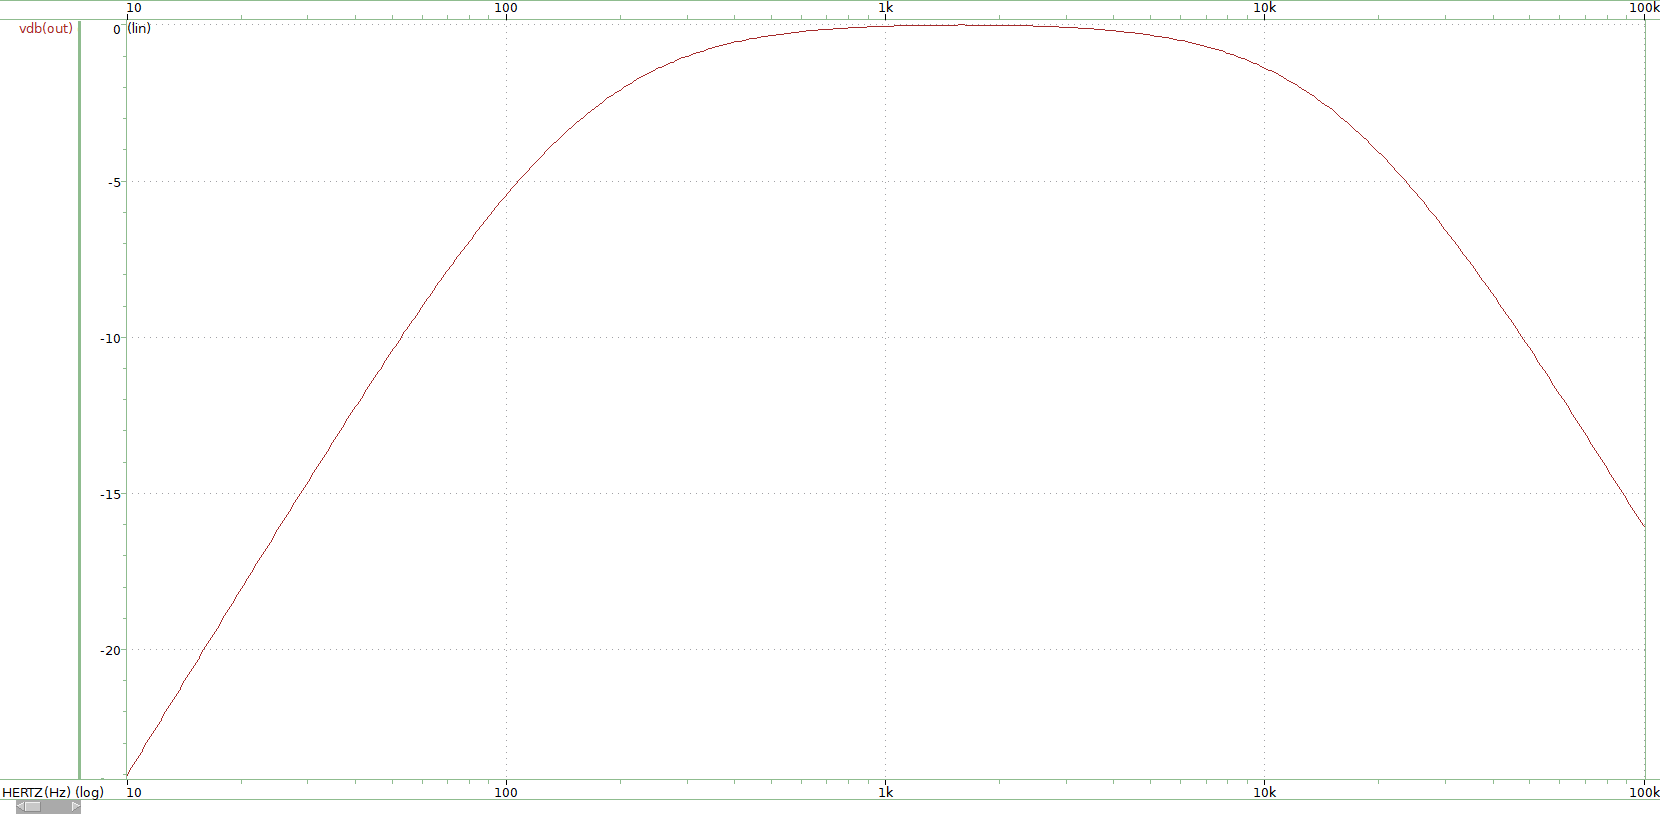
\includegraphics[width=0.70\linewidth]{3_circuito_dif_HSPICE/magnitude_db.png}
\caption{Gráfica de Magnitud en dB de la función de transferencia $H(w)$ obtenida por HSPICE.}
\end{figure}

\begin{figure}[H]
\centering
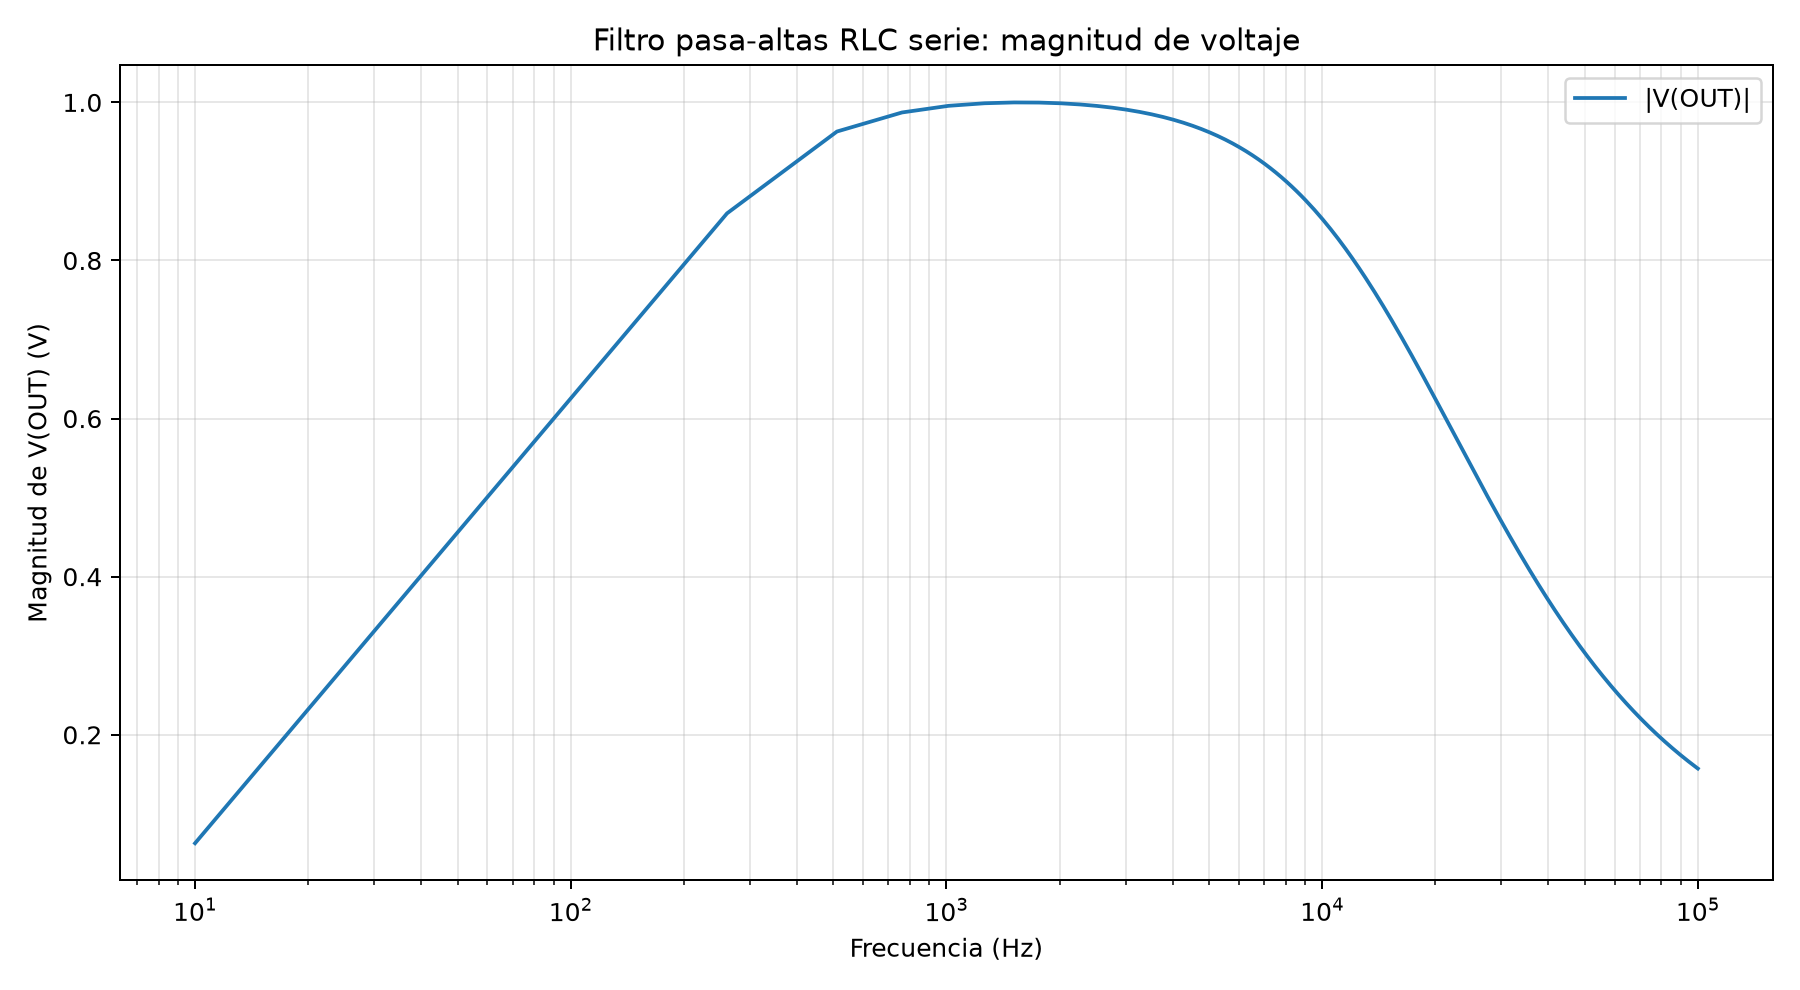
\includegraphics[width=0.70\linewidth]{3_circuito_dif_agent/plots/magnitude_voltage.png}
\caption{Gráfica de Magnitud en Voltaje de $V\_OUT$ obtenida por el agente.}
\end{figure}

\begin{figure}[H]
\centering
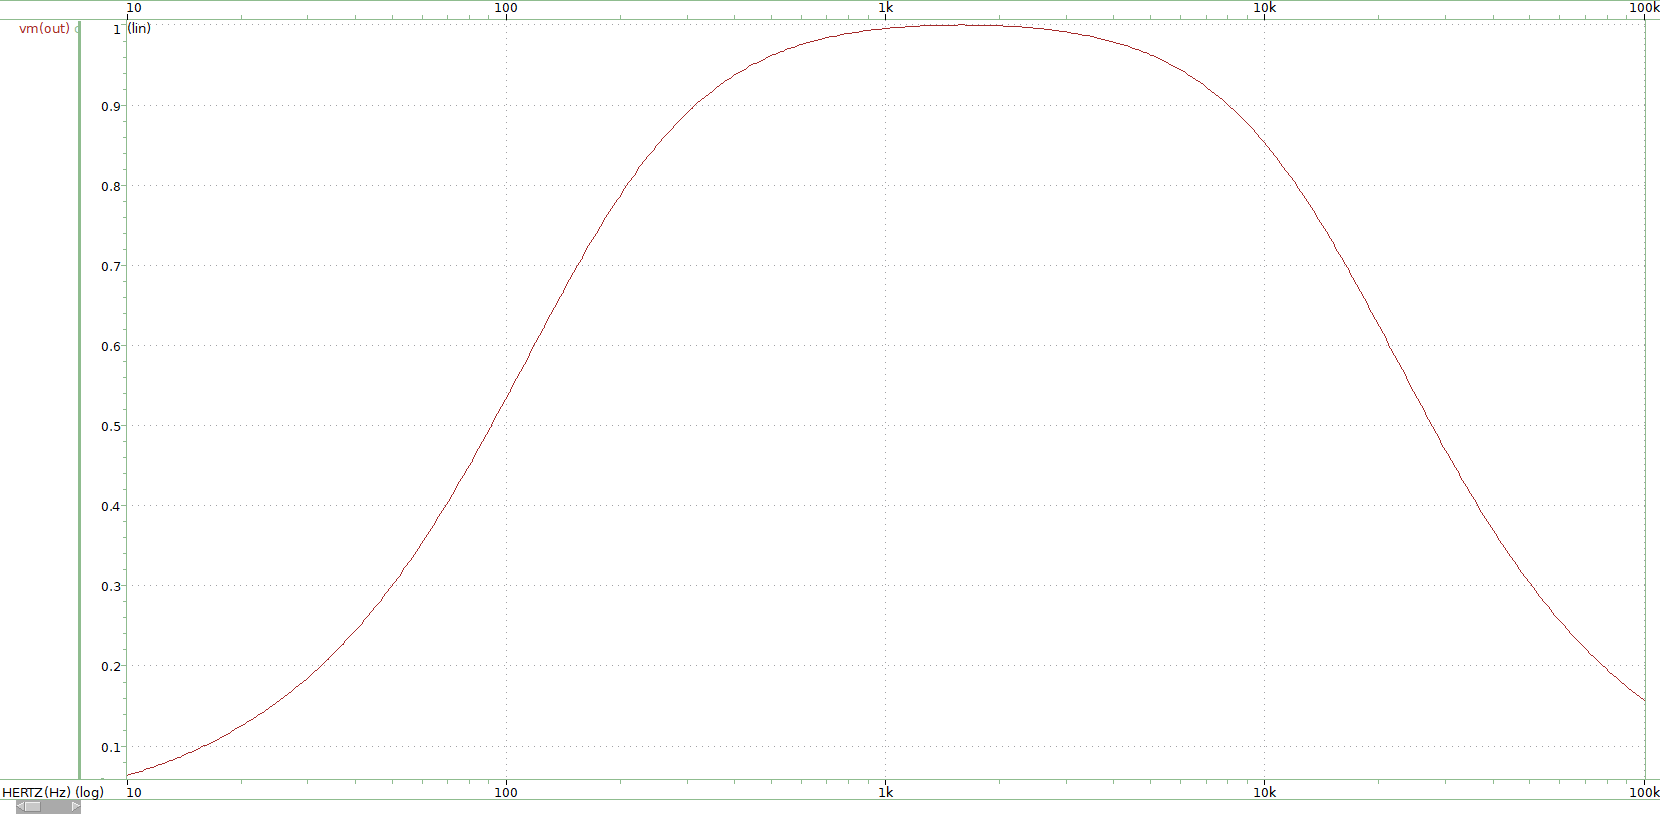
\includegraphics[width=0.70\linewidth]{3_circuito_dif_HSPICE/magnitude_voltage.png}
\caption{Gráfica de Magnitud en Voltaje de $V\_OUT$ obtenida por HSPICE.}
\end{figure}

\begin{figure}[H]
\centering
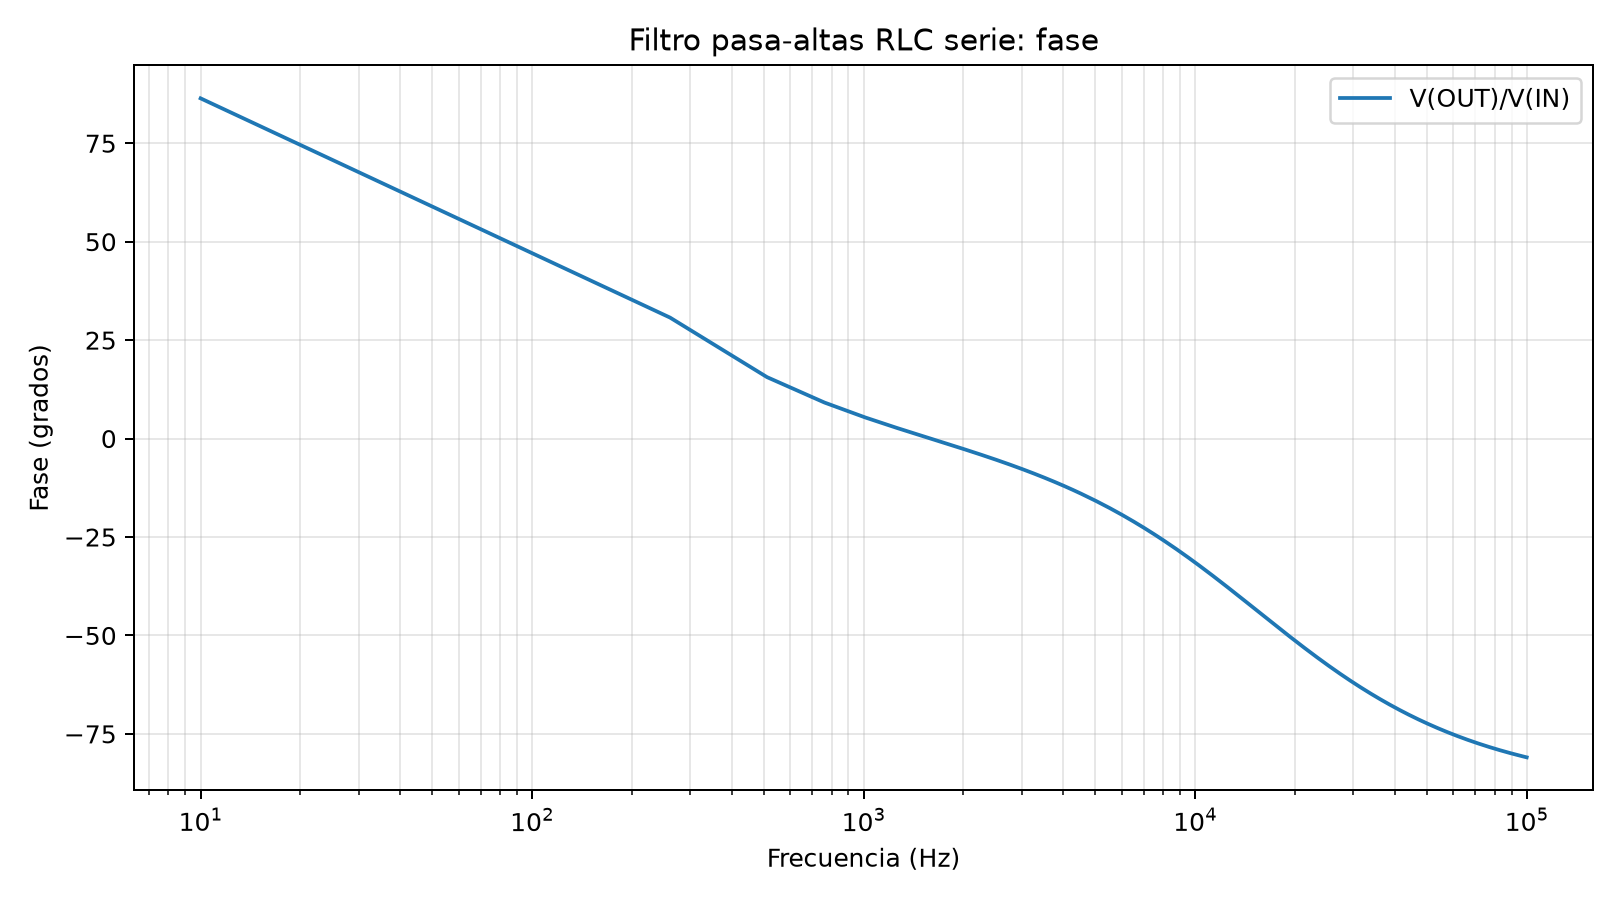
\includegraphics[width=0.70\linewidth]{3_circuito_dif_agent/plots/phase.png}
\caption{Gráfica de Fase de la función de transferencia $H(w)$ obtenida por el agente.}
\end{figure}

\begin{figure}[H]
\centering
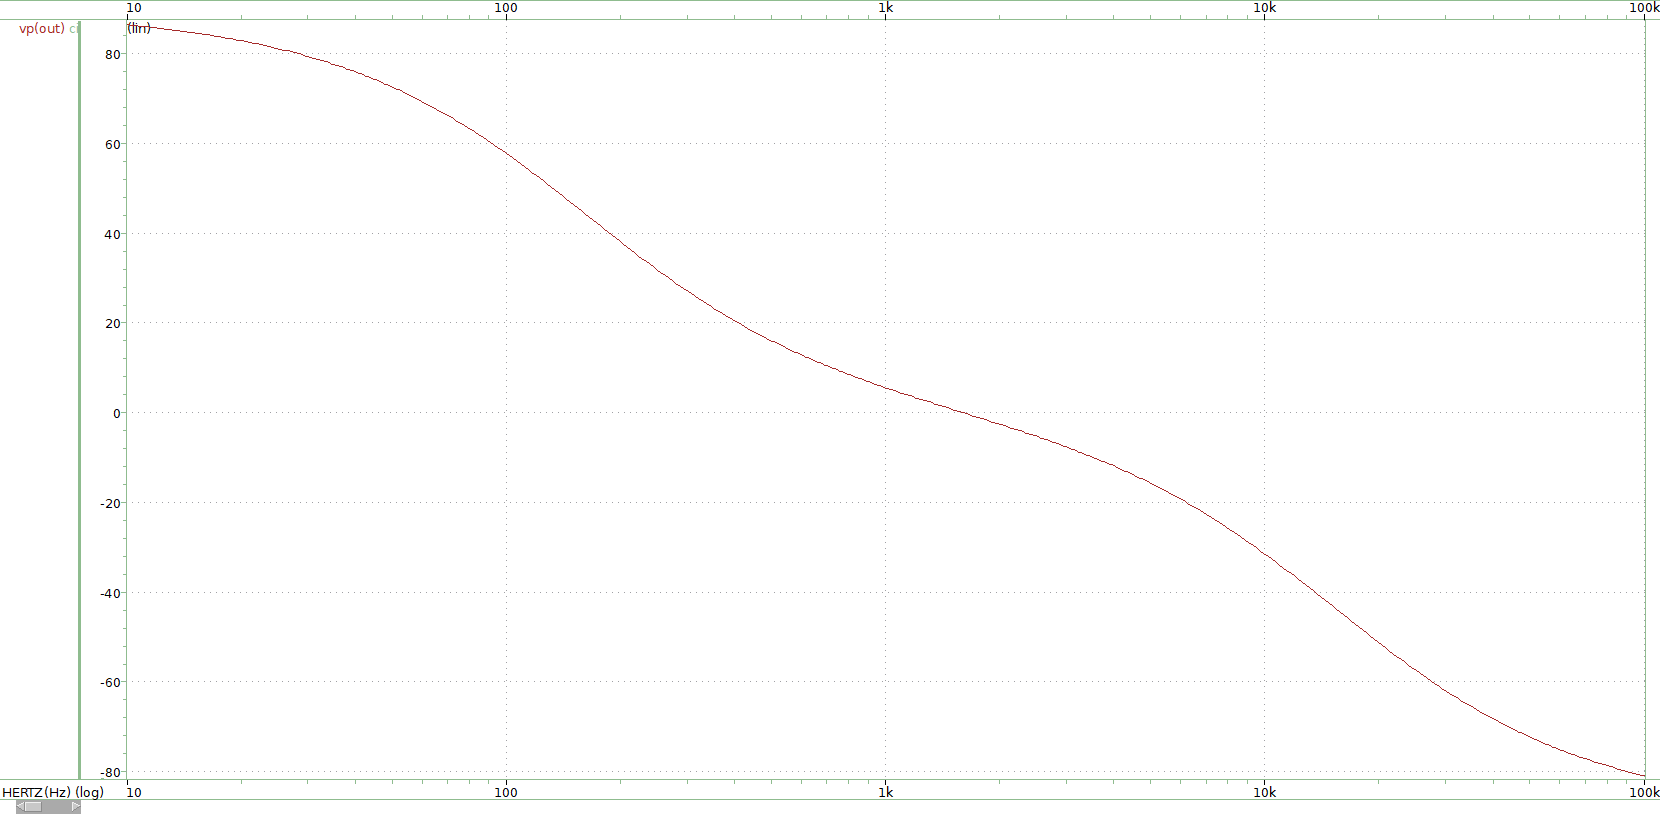
\includegraphics[width=0.70\linewidth]{3_circuito_dif_HSPICE/phase.png}
\caption{Gráfica de Fase de la función de transferencia $H(w)$ obtenida por HSPICE.}
\end{figure}


\subsection{Comparación con HSPICE}
La referencia corresponde a los datos obtenidos por HSPICE usando un circuito RLC, con fuente de entrada de 1 V y barrido DEC de 401 puntos. El agente utilizó un barrido LIN de 400 puntos. Se compararon solo las frecuencias coincidentes exactas de 10 Hz y 100 kHz, sin interpolar ni alterar unidades. En ambas simulaciones, debido a que $V(IN)=1$ V, el voltaje de salida es numéricamente igual a $H(w)=V(OUT)/V(IN)$.

La herramienta \texttt{compare\_reference.py} comparó los fasores complejos de la transferencia, con tolerancias absoluta $10^{-6}$ y relativa $2\times10^{-5}$. Los fasores, errores y estados se transcriben de su artefacto de salida.

\begin{table}[H]
\centering
\small
\begin{tabularx}{\linewidth}{lXX}
\toprule
Frecuencia & Agente $H(w)$ & HSPICE: $H(w)$ \\
\midrule
10 Hz & $3.93262687\times10^{-3}+j6.25872297\times10^{-2}$ & $3.93261262\times10^{-3}+j6.25872707\times10^{-2}$ \\
100 kHz & $2.47167338\times10^{-2}-j1.55260481\times10^{-1}$ & $2.47167003\times10^{-2}-j1.55260522\times10^{-1}$ \\
\bottomrule
\end{tabularx}
\caption{Transferencias complejas en las dos frecuencias coincidentes.}
\end{table}

\begin{table}[H]
\centering
\begin{tabular}{lrrc}
\toprule
Frecuencia & Error absoluto & Error relativo & Estado \\
\midrule
10 Hz & $4.3415\times10^{-8}$ & $6.9231\times10^{-7}$ & \textbf{PASS} \\
100 kHz & $5.3014\times10^{-8}$ & $3.3720\times10^{-7}$ & \textbf{PASS} \\
\bottomrule
\end{tabular}
\caption{Comparación compleja de transferencia; resultado global \textbf{Satisfactorio} (2/2 puntos).}
\end{table}

La comparación cuantitativa cubre únicamente los dos puntos coincidentes; no se afirma equivalencia punto por punto en todo el barrido. Las gráficas HSPICE se incluyen como referencia visual.


La comparación es reproducible con los artefactos JSON de puntos, referencia HSPICE y resultado de \texttt{compare\_reference.py}, conservados en la carpeta de comparación del reporte. % (Caso 3)
% 7_lista_de_entregables.tex
\section{Entregables del Proyecto}

Como parte de las evidencias del proyecto se presentan los siguientes entregables:

\subsection{Repositorio}

Repositorio Git: $https://github.com/Johnngt/Maestria_TSJ/tree/main/Matematicas\_avanzadas/$
$Proyecto\_SPICE$

\subsection{Herramientas de análisis}
 Script Desarrollados: $https://github.com/Johnngt/Maestria\_TSJ/tree/main/Matematicas\_avanzadas/$
 $Proyecto\_SPICE/SPICE\_Educational\_Agent\_First\_6\_Tools$
 
 \small
\begin{longtable}{>{\centering\arraybackslash}p{0.6cm} >{\raggedright\arraybackslash}p{4.7cm} >{\raggedright\arraybackslash}p{10.5cm}}
\toprule
\# & Script & Responsabilidad \\
\midrule
\endfirsthead
\toprule
\# & Script & Responsabilidad \\
\midrule
\endhead
\bottomrule
\endfoot
1 & \texttt{validate\_netlist.py} & Comprueba sintaxis, componentes y directivas admitidos. Emite diagnósticos y estado \texttt{PASS} o \texttt{FAIL}; debe ejecutarse antes de construir el circuito. \\
2 & \texttt{parse\_netlist.py} & Interpreta el netlist validado y genera su representación estructurada. También ejecuta la validación del netlist. \\
3 & \texttt{build\_circuit\_model.py} & Construye el modelo normalizado del circuito, con nodos, ramas, componentes y directivas. \\
4 & \texttt{build\_oriented\_graph.py} & Construye el grafo orientado del circuito y exporta la topología; opcionalmente genera una imagen. \\
5 & \texttt{build\_incidence\_matrix.py} & Genera las matrices de incidencia completa y reducida, conservando el orden de nodos y ramas. \\
6 & \texttt{stamp\_elements.py} & Módulo compartido con los modelos y sellos de los componentes para las formulaciones nodal y Tableau. No es un comando CLI independiente. \\
7 & \url{build_constitutive_matrices.py} & Construye las matrices constitutivas $Y$, $Z$ y el vector $W$ requeridos por Tableau, incluso para una frecuencia AC especificada. \\
8 & \texttt{build\_nodal\_system.py} & Ensambla el sistema nodal clásico para circuitos compatibles. Rechaza fuentes ideales de voltaje y op-amps ideales. \\
9 & \texttt{build\_tableau\_system.py} & Ensambla el sistema Tableau con ecuaciones KCL, KVL y constitutivas. \\
10 & \texttt{build\_mna\_system.py} & Ensambla MNA para la extensión de op-amp ideal del proyecto, incluyendo la restricción entre entradas y la corriente auxiliar de salida. \\
11 & \texttt{solve\_linear\_system.py} & Resuelve sistemas nodales, Tableau o MNA y recupera las variables eléctricas calculadas. \\
12 & \texttt{solve\_ac\_sweep.py} & Ejecuta análisis AC de punto o barrido LIN/DEC; obtiene transferencias complejas, magnitud, decibeles, fase y estado por punto. \\
13 & \texttt{validate\_solution.py} & Valida residuos y consistencia matemática y eléctrica de una solución, incluyendo las ecuaciones correspondientes a la formulación. \\
14 & \texttt{compare\_reference.py} & Compara resultados complejos con un archivo de referencia compatible proporcionado por el usuario. No ejecuta HSPICE. \\
15 & \texttt{generate\_report.py} & Genera un reporte Markdown a partir de un bundle de artefactos calculados y validados. \\
16 & \texttt{plot\_results.py} & Produce imágenes de topología y, con resultados AC, gráficas de magnitud en dB y fase. \\
\end{longtable}
\normalsize

\subsubsection{Scripts de prueba}
\begin{itemize}[leftmargin=*]
  \item \texttt{test\_integration.py}: prueba de integración básica del flujo original de herramientas.
  \item \texttt{test\_extended\_tools.py}: pruebas de regresión para modelos constitutivos, Tableau, análisis AC y reporte.
\end{itemize}

\subsubsection{Flujo general de análisis}
\begin{enumerate}[leftmargin=*]
  \item Validar y parsear el netlist.
  \item Construir el modelo del circuito, su grafo orientado y la matriz de incidencia.
  \item Elegir la formulación compatible: nodal, Tableau o MNA. Para la extensión de op-amp ideal se utiliza exclusivamente MNA.
  \item Ensamblar y resolver el sistema; para AC, procesar cada frecuencia del barrido.
  \item Validar la solución y conservar estados y diagnósticos.
  \item Si existe una referencia externa compatible, compararla cuantitativamente; después generar los reportes y gráficas disponibles.
\end{enumerate}

\subsection{Demo del agente y Netlist final}
Para este reporte se realizó el analisis de 3 circuitos, cuyos archivos generados por el análisis se encuentran en el siguiente path del repositorio:

\begin{enumerate}
\item Caso 1: Circuito Objetivo:

$/SPICE\_Educational\_Agent\_First\_6\_Tools/artifacts/$ ...

$filtro\_activo\_20261116\_1533\_circuito\_objetivo$

\item Caso 2: Circuito Objetivo Modificado:

$/SPICE\_Educational\_Agent\_First\_6\_Tools/artifacts/$ ...

$filtro\_activo\_20261116\_1710\_circuito\_objetivo\_modificado$

\item Caso 3: Circuito Diferente:

$/SPICE\_Educational\_Agent\_First\_6\_Tools/artifacts/$ ...

$filtro\_pasa\_altas\_RLC\_circuito\_dif$

\end{enumerate}

Todos los análisis que se ejecutaron poseen un archivo llamado: \textit{reporte\_ac.md} 
Donde se puede encontrar el netlist que consume el Agente para realizar el analisis, también se encuentra la generación de las diferentes matrices que sostienen el análisis de circuitos como: \textit{Matriz de incidencia}, \textit{Ecuaciones constitutivas}, \textit{Matriz X}, \textit{Matriz Y}, \textit{Vector W}, \textit{Sistema Ensamblado} y \textit{Resultados AC}.

\subsection{Comparación SPICE}

En la sección 4, 5 y 6 se hace la comparación de resultados obtenidos por parte del Agente SPICE y los resultados obtenidos por la simulación del Programa HSPICE.
\section{Conclusiones}
El proposito de esta práctica fue evaluar los resultados obtenidos por un Agente Spice construido con los conocimientos vistos en clase. Adicionalmente el agente AI añadió conocimientos y scripts necesarios para el desarrollo y análisis de esta práctica. Los resultados se compararon con los análisis realizados usando HSPICE, dichos resultados se encuentran en las secciones 4, 5 y 6. 

Como se pudo notar por la evaluación puntual de algunas frecuencias mostradas en la comparación, los valores coinciden con un margen de error muy pequeño en el orden de $x10^{-7}$ esto  nos quiere decir que la similitud entre los valores esperados por parte de la simulación de HSPICE y los valores obtenidos por el agente son muy similares.
Adicionalmente se puede ver visualmente que las gráficas coinciden en comportamiento, siendo muy similares entre si.
Algunas carácteristicas adicionales que proporciona este agente es la obtención del grafo del circuito y matríz de Tableua que representa matemáticamente el circuito analizado.

Por lo que se puede concluir que si se logró realizar un analizador de circuitos tipo SPICE usando un Agente AI en python. Se obtuvieron resulltados muy similares a los de la simulación de HSPICE. Algunas deficiencias que tiene este Agente SPICE sería para simular circuitos más complejos que incluyan transistores y que requieran modelados más complejos.


\end{document}